% figures in chp.tex files need to have paths relative to main.tex
\documentclass[a4paper]{report}

\usepackage{a4}
\usepackage{epsfig}
\usepackage{graphics,graphicx}
\usepackage[lmargin=4cm,rmargin=2cm,tmargin=3.5cm,bmargin=3.5cm]{geometry}
\usepackage{natbib}
\bibpunct{(}{)}{;}{a}{,}{,}
\usepackage{setspace}
\usepackage{amsmath}
\usepackage{amssymb}
\usepackage{amsthm}
\usepackage{amsfonts}
\usepackage{array}
\usepackage{tabulary}
\usepackage{txfonts}
\usepackage{upgreek}
\usepackage{subfig}
\usepackage{float}
\usepackage{longtable}
  \newtheorem{lem}{Lemma}
  \newtheorem{thm}{Theorem}
%\usepackage{lineno}
%\setcounter{page}{1}

%\pagenumbering{arabic}

\usepackage{fancyhdr}

\newcommand{\rr}{\raggedright}
\newcommand{\tn}{\tabularnewline}
\newtheorem{mydef}{Definition}

\begin{document}

\pagestyle{fancy}
\renewcommand{\chaptermark}[1]{%
\markboth{\MakeUppercase{%
\chaptername\ \thechapter.%
\ #1}}{}}
\fancyhead{}
%\fancyfoot{}
\fancyhead[R]{\leftmark}

%\setpagewiselinenumbers



\begin{figure}[htbp]
\begin{center}

\includegraphics[width=7.5cm]{ucllogo.pdf}
\end{center}
\end{figure}

\begin{center}
\begin{huge}\textsc{University College London}\end{huge}
\end{center}
\vspace{2cm}
\hline
\vfill
\begin{center}
{ \huge \textbf{The effects of trade-offs and disturbance on multi-species coexistence} }\\[1cm]
\vfill
\vfill
\large\textbf{Stuart Nattrass}
\end{center}

\begin{center}
\vfill
September 2013\\
\end{center}

\vfill
\begin{center}
A thesis submitted to University College London for the Degree of Doctor of Philosophy\\
\vfill
Department of Genetics, Evolution and Environment\\
University College London\\
Darwin Building\\
Gower Street\\
London, WC1E 6BT\\
\end{center}




\newpage

\vspace*{\fill}

\begin{centering}

\textit{I, Stuart Nattrass, confirm that the work presented in this thesis is my own. Where information has been derived from other sources, I confirm that this has been indicated in the thesis.}

\end{centering}

\vspace*{\fill}


\newpage

%\newpage


%\vspace*{\fill}

%\begin{verse}
%\textit{``Confusion is sex''}\end{verse}\begin{flushright}
%Sonic Youth
%\end{flushright}

%\vspace*{\fill}

\newpage

%\pagenumbering{arabic}

\doublespacing

\chapter*{Acknowledgements}

Thanks to my supervisors, David Murrell and Stephen Baigent, for their guidance, ideas, and inspiration. They have made this entire process an enjoyable one. I have learnt a great deal from both of you, and I am incredibly grateful for everything.

To those who have shared an office, or drinks, with me, thank you for teaching a mathematician biology, and keeping me entertained along the way. Special mentions to Lawrence Bellamy and Aaron Towlson, for welcoming me into the department with pints and open arms, Fraser Murdoch and Claire Asher for keeping the nights out silly, Kate Brown, Pascale Gerbault, and latterly Henry Ferguson-Gow, Tim Lucas and the rest of the Kate Jones group, with whom I shared an office all too briefly. And Jane Dempster, lovely Wo-Ho mum.

Thanks also to my non-science friends, for reminding me that there is a whole world out there.

Finally thanks to Mam and Dad, for putting up with my refusal to stop being a student every step of the way. 

\chapter*{Abstract}


\tableofcontents
\listoffigures
\listoftables

%\pagenumbering{arabic}

%\linenumbers
\chapter*{Introduction}

One of the key issues in ecology is understanding how some communities can maintain high levels of species diversity. In particular, tropical forests and coral reefs are known to support a large number of species, often within a small area. For example, a single hectare of Amazonian forest has been observed to support over 300 species (Valencia et al 1994), while a single region of coral reef ($<15$m$^3$) can host over 75 species (e.g. Smith and Taylor 1972). However, although the preservation of this diversity is a conservation priority (eg REFS), the processes that lead to, and consolidate, this biodiversity are little understood.

Much of the recent theoretical work on this topic has fallen into two categories; niche theory, where species specialise on different resources, and neutral theory, which considers all species ecologically equivalent and dynamics are determined by chance, either demographic or environmental stochasticity. Niche theory can be traced back as far as Darwin, who suggested a deterministic set of events resulting in different species each occupying a unique role within a community (Darwin 1859). More recently, Hutchinson noted the distinction between a species abiotic niche, the range of environments in which it can survive, and the realised niche, a function not only of abiotic factors but also dependent on the identity and actions of other species present in the community (Hutchinson 1958). Theory suggests that for a single resource, the species which can reduce this resource to the lowest level will exclude all other species ($R_0$ REFS), leading to the conclusion that for a given number $n$ of distinct resources, niche specialisation can result in $n$ species coexisting, as each maximises the use of a single resource, while the law of competitive exclusion (Hardin 1960) indicates that $m>n$ species cannot coexist. However, this mechanism often requires an excessive number of distinct resources in order to mirror the biodiversity levels in empirical studies.

 One possible explanation for diversity observed beyond the number of distinct resources is trade-off theory. Since resources are not infinite, no single species can allocate sufficient resource to optimise every life history trait, becoming Law's `Darwinian Demon' (Law 1979). Rather, resources are allocated to one life history trait  at the expense of others, resulting in trade-offs such that, for example, a species that produces seeds with a large mass will produce a much smaller number of seeds (eg Greene and Johnson, Venable), or a species with resource allocation to rapid juvenile growth may do so at the expense of its ability to disperse and colonise other areas in the environment (eg Tilman, Cadotte). Trade-offs such as the competition-colonisation trade-off have been demonstrated to theoretically support an arbitrarily large number of species (Tilman 1994).
 
 Trade-off theory may also be heavily dependent on competitive asymmetry between species. Competitive asymmetry occurs when one individual receives a disproportionate amount of the resource when in competition with another individual. Asymmetric competition is prevalent in insect communities (Lawton and Hassell 1981), and is also common within plants, where competition for light is expected to be dependent on size, with the larger individual intercepting large quantities of light at the expense of a smaller neighbour (Weiner 1990). Competition is said to be highly asymmetric if a small difference between individuals results in a large difference in the amount of resource garnered from competition.
 
 In Chapter 1, we examine the effects of this competitive asymmetry on the likelihood of coexistence. Using a Lotka-Volterra type model of competition, we find analytical conditions for the coexistence of two species along a fecundity-competition trade-off. We demonstrate that competitive asymmetry must be sufficiently high if the system is to support two or more species, and show that the likelihood of two species coexistence increases with competitive asymmetry, being maximised when competition is given by a discontinuous step function. Further, using this step function, we show analytically that this trade-off can support any number of species, although the probability of the system supporting randomly selected species declines rapidly as the number of species increases.
 
 While niche theory focuses on the differences between species, neutral theory instead considers all species equivalent at an individual level (Hubbell 1979), with community structure determined by chance. Designed as null models for coexistence, neutral theory models have proven able to predict high levels of biodiversity (REFS), and has accurately captured a range of observed relative abundance distributions (REFS). One type of model that utilises many of the assumptions of neutral theory are lottery models, introduced by Sale (1977) and developed further by Chesson (YR), where space is considered a limiting factors and the occupation of sites by a species is determined by the proportion of sites occupied by that species.

In Chapter 2, we develop a lottery type model in which we combine aspects of both neutral and niche theories. Using a trade-off between fecundity and juvenile growth rate, we introduce species specific characteristic into a stochastic model where  allocation of space is subject to significant environmental stochasticity. We demonstrate that this combination of species specific traits and chance can lead to coexistence of at least two species competing asymmetrically for light, and using stochastic boundedness as a criteria for coexistence, find express conditions for this coexistence. 

Further, we use this stochastic model to study the effects of disturbance on the community structure. Disturbance has been suggested as a strong driver of biodiversity, by perturbing the system such as to prevent the realisation of a lower diversity equilibrium situation (e.g. Sousa 1984, Denslow 1987). These events, defined by Shea et al. (2004) as events that alter niche opportunities via the death of large numbers of individuals, can create an environment where space limited species, such as pioneers, that prosper in an unsaturated environment, can persist in regions where they would otherwise by excluded if disturbance was too weak. If disturbance levels are sufficiently high, however, those species that are strong in saturated and congested environments will be excluded, as the environment will favour space limited species. Using these arguments, the intermediate disturbance hypothesis (IDH) suggests that diversity will be maximised at intermediate levels of disturbance, producing a unimodal, peaked diversity-disturbance relationship (DDR) (eg Connell 1978, Grime 1973, Huston 1979). However, empirical evidence for the IDH is mixed (see review in Mackey and Currie 2001), while it has also attracted theoretical criticism (e.g. Fox 2012). We expand our model to include disturbance events determined by two factors, frequency and intensity (proportion of individuals killed), and find that disturbance can dramatically increase the range of parameters for which two species can coexist. We demonstrate that the aspect of disturbance measured can have very different effects on the observed DDR, such that the peaked DDR predicted by the IDH is just one of several possible results from the same mechanism, and show that system capacity, the maximum number of individuals supported in the community, is crucial in determining how the community will react to disturbance.

While the focus of the work presented in Chapter 2 is a fecundity-growth trade-off, there are three main life history traits to consider for plants - fecundity, growth and defence against herbivory or other disturbance (REF). Therefore, in Chapter 3 we adapt the stochastic model in order to consider trade-offs between different combinations of these three traits, by introducing species specific disturbance intensities. We then compare the likelihood of these different trade-offs allowing two species coexistence, and compare the resulting predictions to empirical evidence from the literature. We find that using the lottery model framework, trade-offs including growth rate differences between species can support coexistence for any system capacity, while a trade-off between fecundity and defence cannot sustain more than a single species in large systems, and this is supported by the empirical results, showing no relationship between fecundity and defence, while growth-defence and fecundity growth trade-offs are observed in natural communities. By correlating the species specific intensities, we demonstrate that the fecundity-growth trade-off is likely to contribute the most to coexistence.

Using these conclusions, we then extend the stochastic model in Chapter 4 to include a third species along a fecundity-growth trade-off, and examine the effects of disturbance with greater than two species. Introducing a third species allows the consideration of coexistence between specialist species (with high fecundity or rapid juvenile growth rate) and a generalist with intermediate seed production and growth rates. We examine the effects of varied trade-offs and disturbance regimes, and introduce regions of the community that may be protected from disturbance, or experience a different disturbance regime from the remaining forest sites. We show that these refuges can provide for species that would otherwise be excluded if exposed to the conditions in the rest of the community, suggesting that disturbance regimes alone can allow native species to survive the invasion of an invasive species. Further, the model predicts that the effectiveness of nature reserves may be best observed in the regions neighbouring a reserve, rather than within the reserve itself. The potential effects of management strategies on species richness are then considered.

This thesis seeks to address the issues of determining both the type of competition best capable of sustaining a diverse community, and the predicted effects of disturbance regimes on species richness. These two processes aim to form preliminary steps towards a full mechanistic understanding of how diversity is maintained.



\newpage
\chapter{Quantifying the probability of coexistence in communities with asymmetric competition}
This work was previously published in Bulletin of Mathematical Biology (Nattrass et al 2012)
\newpage
\topskip0pt
\vspace*{\fill}
\section*{Abstract}
Trade-offs in performance of different ecological functions within a species are  commonly offered as an explanation for coexistence in natural communities. Single trade-offs between competitive ability and other life history traits have been shown to support a large number of species, as a result of strong competitive asymmetry. We consider a single competition-fecundity trade-off in a homogeneous environment, and examine the effect of the form of asymmetry on the likelihood of species coexisting. We find conditions that allow coexistence of two species for a general competition function, and show that (1) two species can only coexist if the competition function is sufficiently steep when the species are similar; (2) when competition is determined by a linear function, no more than two species can coexist; (3) when the competition between two individuals is determined by a discontinuous step function, this single trade-off can support an arbitrarily large number of species. Further, we show analytically that as the degree of asymmetry in competition increases, the probability of a given number of species coexisting also increases, but note that even in the most favourable conditions, large numbers of species coexisting along a single trade-off is highly unlikely. On this basis we suggest it is unlikely that single trade-offs are able to support high levels of biodiversity without interacting other processes.
\vspace*{\fill}
\newpage

\section{Introduction}


There is no such thing in the natural world as a Darwinian Demon which maximises all possible life history traits \citep{law1979optimal}, and instead individuals have to allocate resources to one life-history trait at the expense of others. This results in trade-offs between life history traits, so that, for example, a plant species which allocates resource to rapid growth does so at the expense of its ability to withstand shading; or a species that has allocated much of the available resource to out-competing other species will suffer a decrease in its ability to disperse and colonise empty areas of the environment  \citep[e.g.][]{tilman1994competition, cadotte2006testing}. Other classic life-history trade-offs include the offspring size-number trade-off \citep[e.g.][]{venable1992size}; the trade-offs between pathogen resistance and fecundity \citep[e.g.][]{bowers1994life}; and competition and intra-guild predation \citep{amarasekare2007trade}.

Theory has shown that these trade-offs can allow two or more species to coexist while competing for the same resources  \citep[e.g.][]{kisdi2003coexistence, levins1971regional, bonsall2004life}, and consequently that trade-offs may be instrumental in the evolution of biodiversity \citep{schluter1995adaptive, white2005adaptive, bonsall2004life}. In particular, \cite{levins1971regional} originally highlighted two such trade-offs, the competition-colonisation trade-off which has received much attention, and the trade-off between death rate and competitive ability which has received less attention. Levins and Culver argued that two species can coexist if one experiences a lower death rate, but is a weaker competitor than the other species. Both trade-offs are closely related, and have received much attention, with \cite{tilman1994competition} showing that the competition-colonisation trade-off can potentially lead to infinitely many species coexisting.

However, the conditions under which species either competitively exclude, or coexist alongside others due to trade-offs between competition and other life history traits might also be dependent on the existence, and level, of asymmetric competition between species \citep{adler2000space}. Competition is called asymmetric if an individual with larger trait value (e.g. size) is bestowed some benefit over small trait valued neighbours, winning more than 50\% of contests by virtue of this difference in trait. This competition is deemed to be very asymmetric if there is a large difference in competitive ability between individuals which have slightly different trait values. Asymmetric competition is widespread in the natural world, forming the majority of inter-species competition in insects \citep{lawton1981asymmetrical}; and is prevalent in plants where competition for light is expected to be size dependent, such that a larger plant may intercept nearly all the available light at the expense of a smaller individual \citep{weiner1990asymmetric}. However, there is relatively little theory that investigates how the strength of competitive asymmetry may affect the maintenance of biodiversity.

\cite{adler2000space} demonstrated that, if the competition between two species is determined by a step function with infinite gradient when traits are the same, then the species richness, the number of species present in the community, is maximised in their model. They then used numerical simulations of their model to show how reducing the degree of competitive asymmetry reduces the number of species that can coexist on the trade-off. Similarly,  \cite{kisdi1999evolutionary} showed that the gradient of the competition function at the point where two competing individuals have the same trait value (i.e. the same size), is critical in determining the number of species that may evolve in the long term. In other words, coexistence and the evolution of a large community seem to be more likely if a small change in fecundity translates into a large change in competitive ability.

Here we build on this  previous work and analyse a model with a single trade-off between competitive ability and fecundity. We will find conditions required for two species to coexist, and demonstrate that while no more than two species can coexist when competition is a linear function of the trait value, if the mechanisms of the competition between species allows for a discontinuity in the competition function, then coexistence of any number of distinct species is possible. We also demonstrate analytically for two species that this discontinuous competition gives an upper bound on the likelihood of coexistence when compared with two convex-concave functions that tend to the step function as parameters are altered. Niche theory suggests that as species become more similar coexistence should become more unlikely, but few studies have quantitatively investigated this in the context of life-history trade-offs. Using rigorous proofs we will show that competitive asymmetry and the gradient of the competition function at the origin are important in determining the number of species able to persist on one trade-off, but also show that even under the most favourable conditions, large numbers of species coexisting on one trade-off is very unlikely.
 
\section{The Model}

We examine coexistence criteria in a simple model where species differ only in their per capita fecundity and their competitive ability. The per capita fecundity is compared to competitive ability through assigning a trait value to each species. The typical traits we have in mind are body size, or weight of armament, and a strong competitor has a lower fecundity, creating a competition-fecundity trade-off. In doing so we assume a species which is a stronger competitor diverts resources into this trait, perhaps by delaying reproduction and growing in size; whereas a weaker competitor diverts more resources into reproduction at the cost of competitive ability. We assume this trade-off, which restricts parameter space within the model, is conserved across species, and that it can be described by two functions that relate a species' trait value to (i) fecundity, and (ii) competitive ability. In particular, we will explore how the shape of the latter function is important in determining the amount of species that may be supported by the trade-off.


Let $n$ denote the number of species present in the environment, with species $i$ having expected size $x_i$ and population density $N_{x_i}$. We use Lotka-Volterra equations to describe the population dynamics:
 \begin{equation}
\label{model}
 \frac{d N_{x_i}}{dt}=N_{x_i}\left( p(x_i) - \sum_{j=1}^n c(x_i - x_j)N_{x_j}\right),
 \end{equation}
where $p(x_i)$ is the intrinsic growth rate of species $i$ when resources are not limiting and the environment is free of competition;  $c(x_i-x_j)$ is the competition kernel used to quantify the impact of competition with species $j$ on species $i$ which depends only on the difference in trait values $x_i-x_j$. For larger species, which have lower fecundity, $p(x_i)$ is lower than for species with smaller trait values, so we assume that  $p(x_i)$ is a strictly decreasing non-negative function of trait value  $x_i$. The intrinsic growth rate $p$ is assumed to be greater than zero, as any species with a non-positive growth rate would not be able to grow in even an empty environment. Since we are at liberty to choose units for $x$, we choose $x_{max}=1$ since the maximum trait value for which the growth rate is zero: $p(1)=0$. Similarly, we let $x_{min}=0$ be the smallest permissible trait value, meaning all extra resources are diverted into fecundity rather than competitive ability. In what follows we will mainly work with the linear growth function  $p(x_i)=\rho(1- x_i)$ where $\rho>0$. However, we will use $ p(x_i)$ wherever possible in order to show how the method may be extended to nonlinear growth functions. Using these assumptions, our aim is to investigate the possibility and probability of coexistence of species selected at random across the entire trait-space.

The continuous competition kernels $c(x_i - x_j)$ we consider are non-increasing functions of the difference between the individual's trait value and that of its competitor, i.e. non-increasing in $(x_i-x_j)$. This means that an individual with large trait value experiences little competition from competing individuals with smaller trait values, while small trait value individuals suffer a much larger competitive effect from large individuals. For example, taller trees will clearly intercept light earlier than shorter individuals, while shading shorter neighbours. However, shorter trees will have limited shading effect on a tall neighbour. We use convex-concave functions, to reflect the realistic assumption that two large species will have a similar effect on a much smaller third species, while a large individual will suffer approximately equal effects from two much smaller individuals. However, when all three species are of similar size, the effects of the larger (smaller) two on the smallest (largest) may vary significantly. The discontinuous competition is a suitable limit of such continuous functions, and although it is less realistic, it allows for useful analytical upper bounds for the continuous cases.

We study the effects of asymmetric competition for two species considering (1) a general function $c(z)$ and linear growth, with a focus on two examples; and (2) for general growth  $p(x_i)$ with linear and step function $c(x_i - x_j)$, which we also consider for $n>2$. As with the growth function, the general linear competition kernel is studied, with
 \begin{equation}
 \label{linearc}
 c(x_i - x_j)=\kappa - \theta (x_i - x_j),
 \end{equation}
but additional restrictions are applied to the convex-concave and step functions model. To ensure that the effect of this competition is never positive, such that the model represents a predator-prey interaction or mutualism, it is necessary to have $\kappa>\theta$. The intraspecific competition (i.e. when $x_i=x_j$) is assumed to be identical across species, and can be scaled to one to reduce the number of parameters, and it is assumed that the total negative effect of competition in an interaction between any two individuals is the same. Ecologically, this means that there is a set amount of resource to be shared between any two individuals. When the two individuals are the same species and have equal trait values, each takes on average 50\% of the resource, or wins the competitive contest roughly half of the time. When the trait values differ, the stronger competitor takes a greater percentage of the resource, leaving less for the weaker competitor. To reflect this we study two continuous competition functions, a piecewise linear function given by 
\begin{equation}
\label{pwlcomp}
c(x_i-x_j)=\begin{cases}
1+\epsilon & x_i-x_j\leq-\Theta \\
1-\frac{\epsilon}{\Theta}(x_i-x_j) & -\Theta<x_i-x_j<\Theta \\
1-\epsilon & x_i-x_j >\Theta, 
\end{cases}
\end{equation}
and a smooth function modified from that used by \cite{kisdi1999evolutionary}, which we consider as
\begin{equation}
\label{kisdimodified}
c(x_i-x_j)=1+\epsilon -\frac{2\epsilon}{1+e^{-\frac{2(x_i-x_j)}{\Theta}}}.
\end{equation}
As $\Theta$ tends to zero, these two functions both tend to a step function, that will be considered in detail for general $n$ species dynamics. This  function is given by
 \begin{equation}
 \label{stepc}
 c(x_i - x_j)=\begin{cases}
 1+\epsilon & x_i <x_j \\
 1 & x_i = x_j \\
 1-\epsilon & x_i > x_j
 \end{cases},
 \end{equation}
and is used as the discontinuous competition function throughout this study \citep[see also ][]{tilman1994competition, may1994superinfection}.
 
Our model is similar to those studied by \cite{law1997evolution} and \cite{kisdi1999evolutionary}, although both of their models only considered a concave-convex competition function in lieu of the linear and discontinuous functions considered for large $n$ here. The function $c_{k,\nu}(z) =  c(1-1/(\nu+e^{kz}))$ used by Kisdi, of which \eqref{kisdimodified} is a modified version tends to a discontinuous step function of the type studied here as $\theta = 1/k$ tends to zero ($\nu>0$ fixed). The use of simplified competition functions in this study allows for more analytical work than the more complex functions used in Kisdi's analysis. We demonstrate in the two species case that our results for the discontinuous competition function are similar to those produced using the competition kernel given by \eqref{kisdimodified} when $\theta$ is small, and hence allow for comparison with Kisdi's competition model which shows qualitatively similar results for two species coexistence with linear growth.

When $\epsilon=1$, our model with a step function $c(z)$ takes the same form as the spatially implicit model presented by \cite{klausmeier1998extinction}, which also demonstrates that coexistence is possible for general $n$. However, this current study builds upon this work to indicate both the likelihood of this coexistence, and the effects of weakened asymmetry in competition.

Before studying the effects of trade-offs on the coexistence of species, it is important to clarify what we mean by coexistence. In its strongest sense, coexistence can be taken to mean that all species present persist at a given positive equilibrium value. This means that any mathematical model of the system will exhibit coexistence if and only if there is a positive fixed point that is globally asymptotically stable, in the sense that all initial conditions for which each species has positive density end up at a positive equilibrium density. This is the notion of coexistence used by  \cite{strobeck1973n}. \cite{law1996permanence} uses a less stringent definition of coexistence, namely that the system exhibits coexistence if all species densities remain bounded and for all positive initial densities, there is a  density $\delta>0$ such that all the species eventually exceed $\delta$, demonstrated mathematically by the concept of permanence. In this study, a collection of species is considered to exhibit coexistence if the model of those species exhibits permanence. However, as permanence is an immediate consequence of a globally asymptotically stable equilibrium in the interior, the existence of the latter is used to show coexistence in our discontinuous competition model.

In later sections we study n-species communities and investigate the likelihood of coexistence given the model, and the trade-off function. Here we assume communities are assembled randomly from a regional species pool where all species (trait values) are present. We note that our results will be different to the expected number of species that will evolve via small mutations from a mono-specific community; or from community assembly by invasion of species one at a time; but in both cases relatively high levels of coexistence are required for large communities to occur.

\section{Results}

\subsection{Linear Competition}
Suppose that the competitive advantage held by one species over another is a linear function of the difference between the trait values of the two species. Then the competition coefficients $c(x_i -x_j)$ in \eqref{model} are determined by use of the function given in \eqref{linearc}. In order to preserve the competition-fecundity trade-off, it is necessary that as fecundity decreases - and the function $p(x_i)$  decreases - the competitive advantage that the species holds over a fixed, weaker competitor is increasing. This translates to the mathematical condition $\theta>0$. To simplify the calculations, it is assumed that $x_i>x_{i+1}$, but the results shown apply to any ordering of species, and therefore trait values. 
The equations for the two species system are
\begin{eqnarray*}
\frac{dN_{x_1}}{dt} & = & N_{x_1} \left\{ p(x_1) - \kappa N_{x_1} - (\kappa-\theta(x_1-x_2))N_{x_2} \right\}\\
\frac{dN_{x_2}}{dt} & = & N_{x_2} \left\{ p(x_2) - (\kappa-\theta(x_2-x_1))N_{x_1}-\kappa N_{x_2}\right\}.
\end{eqnarray*}

This model admits an interior fixed point when
\begin{equation}
\label{lin2dposfp}
 \frac{\kappa}{\theta}\frac{p(x_2)-p(x_1)}{p(x_2)}<x_1-x_2< \frac{\kappa}{\theta}\frac{p(x_2)-p(x_1)}{p(x_1)},
 \end{equation}
and this is globally stable  whenever it exists, since $\kappa>0$ by assumption. Therefore, coexistence is possible if the condition \eqref{lin2dposfp} is satisfied.

However, the limits of linear competition in giving rise to coexistence are shown if a third species is introduced to the system. We now demonstrate that regardless of the trait value this species holds, or the parameter values for $\kappa, \theta$, it cannot form a permanent three species system with the two already species present.  

Note that when equation \eqref{linearc} is used, the $3\times 3$ matrix of competition coefficients has a determinant of zero, i.e. is singular, and that therefore the model does not have a unique equilibrium point in the interior. In Lotka-Volterra systems, this means that the system does not exhibit permanence \citep[Theorem 13.5.1 in ][]{hofandsig}.

Therefore, no third species can form a permanent coalition with the two species already present. We conclude that with a linear function for competition, a maximum of two species can stably coexist and when a third species is introduced, the model exhibits neither asymptotic stability nor permanence. The linear trade-off case is degenerate, but it is useful in illustrating the dependence of the model on the form of the competition function. We therefore switch our attention to a model utilising a nonlinear competition function.

\subsection{Generalised Competition in the two species case}
Consider a generalised competition function $c(x_i - x_j)=c(z)$, which is decreasing, such that $c�(z)\leq0$ for all $z$, for two species. These species are different in two aspects, competitive ability and population growth rate (effectively $K$ and $r$ respectively), both of which are determined by a single parameter $x_i$ for species $i$. We assume that growth rate decreases linearly with $x_i$, such that $x_i$ can be considered as the proportion of non essential resource dedicated to competitive strength at the expense of population growth rate. It is simple to scale the model such that we can define this growth rate by the function $p(x)=1-x$. This therefore means that competitive ability must increase with $x_i$ when the second species remains unchanged. We assume that the competition coefficients are a function of $x_1-x_2$, so therefore can be treated by a function $c(z)$ of a single variable $z$. The competition coefficient $c_{ij}$ gives the negative effect of species $j$ on species $i$, and is defined by $c(x_i-x_j)$. This means that $c(z)$ must be a monotonically decreasing function of $z$. Note the model can be scaled to ensure $c(0)=1$ without any loss of information. 

If two species have identical competitive ability, but differ in growth rate, then the faster growing species would competitively exclude the slower grower, so an essential condition for coexistence is that $c'(0) <0$. 
 
Therefore, the system is given by
\begin{equation}
 \dot{N_1}=N_1\left(1-x_1 -N_1-c(z)N_2\right),
\end{equation}
\begin{equation}
  \dot{N_2}=N_2\left(1-x_2 -N_2-c(-z)N_1\right).
  \end{equation}
  where $z=x_1-x_2$. The condition for global stability of an interior fixed point is then given by $c(z)c(-z)<1$, which is therefore a further condition on the function $c(z)$ for coexistence in the 2-species case.

It is simple to show that an interior fixed point is present when 
\begin{align}
1-x_1-c(z)(1-x_2)&>0, \\
1-x_2-c(-z)(1-x_1)&>0. \end{align}
By writing these as functions of $z$ and $x_2$, it is possible to rearrange to get
\begin{align}
\label{x2upper}
x_2&<\frac{1-z-c(z)}{1-c(z)} \\
\label{x2lower}x_2&>\frac{(1-z)c(-z)-1}{c(-z)-1} \end{align}
We now assume without loss of generality that species 1 is the competitively dominant species, i.e. $z>0$. Then if we define $z^*$ such that
$
1-z^*-c(z^*)=0$
and $\hat{z}$ such that
$1-(1-\hat{z})c(-\hat{z})=0,$
 (defined uniquely for convex-concave functions where $z c''(z)>0$ for $z\neq0$ and $c'(0)<-1$),
then the area of coexistence can be found by
\begin{equation}
\label{areacoexist}
2\left( \int^{z^*}_0 dz \frac{1-z-c(z)}{1-c(z)} - \int^{\hat{z}}_0 dz \frac{(1-z)c(-z)-1}{c(-z)-1} \right)
\end{equation}
where the factor of 2 is to include the other ordering of traits. It is relatively simple to show that with these assumptions, coupled with the fact that $c(-z)+c(z)=2$, coexistence is only possible if $c'(0)<-1$ (Appendix~\ref{appendix1a}). This is in accordance with the work of Adler and Mosquera, who state that monoculture will prevail when the steepness of the competition curve has magnitude less than 1.

As an example, we use the modified version of the function used by \cite{kisdi1999evolutionary} given by \eqref{kisdimodified}, scaled such that the intraspecific competition coefficients are unity, and the parameter $\epsilon$ measured the greatest level of dominance possible, so $c(z) \in [1-\epsilon,1+\epsilon]$ for all $z$.  There is an issue in that $z^*$ and $\hat{z}$ as defined above cannot be found by simply rearranging these equations. However, as demonstrated in Figure~\ref{kisdipic}, when we numerically find the area of the region of coexistence, this area monotonically decreases as the parameter $\Theta$ is increased. The likelihood of coexistence is maximised at $\Theta=0$, where the competition coefficients are determined by a step function. Using Taylor series expansions of the functions $F_1(z)=1-z-c(z)$ and $F_2(z)=(1-z)c(-z)-1$, we can show that the area of coexistence tends to the results presented in Section~\ref{discontresults} as $\Theta$ approaches 0.

\begin{figure}[htbp]
   \centering
   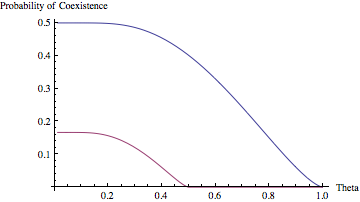
\includegraphics[width=4in]{kisdinum}
   \caption[How the probability of coexistence changes with the slope of the competition kernel at the origin]{\textbf{How the probability of coexistence changes with the slope of the competition kernel at the origin:} The probability of coexistence given by the convex-concave function \eqref{kisdimodified} changes with the parameter $\Theta$, which determines the steepness of the curve at $z=0$. Shown are the cases $\epsilon=1$ and $\epsilon=1/2$.}
   \label{kisdipic}
\end{figure}
 
As a further example, we can investigate the piecewise linear function \eqref{pwlcomp}, where pairs of species with similar trait values will have different effects on one another than pairs with different trait values, but that once a threshold of dissimilarity is passed, all species have the same effect on one another.  Note that this approximates the smooth function \eqref{kisdimodified} considered above. This gives two cases, as the function $(1-z)^{-1}$ will cross $c(-z)$ on the constant part for small $\Theta$, but the sloped part for slightly larger $\Theta$. The two cases are  that where $\Theta<\frac{\epsilon}{(1+\epsilon)}$ and that where $\frac{\epsilon}{(1+\epsilon)}<\Theta<\epsilon$. In the case where $\Theta$ is small, we can write the above integrals as
\[
2\left(\int_0^\Theta \frac{\epsilon-\Theta}{\epsilon}dz + \int_\Theta^{\epsilon} 1-\frac{z}{\epsilon}dz-\int_0^\Theta \frac{\epsilon-\Theta}{\epsilon}-z dz -\int_\Theta^{\frac{\epsilon}{1+\epsilon}} 1-\frac{1+\epsilon}{\epsilon}z dz\right)\]
\[= 2\left(\Theta-\frac{\Theta^2}{\epsilon}+\frac{\epsilon}{2}-\Theta+\frac{\Theta^2}{2\epsilon}-\Theta+\frac{\Theta^2}{\epsilon}+\frac{\Theta^2}{2}+\frac{\epsilon}{2(1+\epsilon)^2}+\frac{\epsilon^2}{2(1+\epsilon)^2}-\frac{\epsilon}{1+\epsilon}+\Theta-\frac{\Theta^2}{2}-\frac{\Theta^2}{2\epsilon}\right)\notag
\]
\[=\frac{\epsilon^2}{1+\epsilon}\]
For larger $\Theta$, we can write the integrals as
\[
2\left(\int_0^\Theta \frac{\epsilon-\Theta}{\epsilon}dz + \int_\Theta^{\epsilon} 1-\frac{z}{\epsilon}dz-\int_0^{\frac{\epsilon-\Theta}{\epsilon}} \frac{\epsilon-\Theta}{\epsilon}-z dz\right) \]
\[=2\left(\Theta-\frac{\Theta^2}{\epsilon}+\frac{\epsilon}{2}-\Theta+\frac{\Theta^2}{2\epsilon}-\frac{1}{2}+\frac{\Theta}{\epsilon}-\frac{\Theta^2}{2\epsilon^2}\right)\notag 
\]
\[
=\frac{(\epsilon-\Theta)(\Theta+\epsilon(\epsilon+\Theta-1))}{\epsilon^2}.
\]
We therefore find that the probability of two species coexisting is constant for small $\Theta<\epsilon/(1+\epsilon)$, and a decreasing function of $\Theta$ when the competitive difference between similar species is smaller, i.e. when $\Theta$ is larger. Because in both this in the concave-convex case, the step function limit serves to maximise the probability of two species coexisting, we now consider the discontinuous case in more detail, as this will give an upper bound on the probability of coexistence for $n$ species.

\subsection{Discontinuous Competition}
\label{discontresults}
In a similar model to that presented here \cite{adler2000space} demonstrated how species richness increases with the gradient of the competition function at the origin (i.e. when two individuals have the same trait value), and this is supported by our results above. The logical extreme of this is that likelihood of coexistence will be maximised if the gradient at the origin is infinite, and we therefore now consider a step function for the competition coefficients, as given by \eqref{stepc}. We note that \cite{nowak1994superinfection} used a very similar model, although they were studying the effects of superinfection on virulence in parasites rather than the number of different strains or species that the model could support. We recognise that such a competition gradient is unlikely to be found in nature (although \cite{kubota1995tree} found limited evidence of total competitive asymmetry in trees species in Northern Japan), but it is mathematically convenient to use this function to analytically investigate upper bounds for the  levels of biodiversity that can be supported on a single trade-off. As illustrated for the two species case above, our results will be very close to the case where the competition function is that used by Kisdi, and the piecewise linear function, mentioned above when $\Theta$ is small, and also to the competition-colonisation trade-off model of \cite{tilman1994competition} that assumes completely asymmetric competition between individuals of different trait values. Biologically, a species requires a positive growth rate $p(x_i)$ in order to be able to fixate in the environment even in the absence of competition. Therefore,  the range of trait values $x_i$ is restricted such that for all possible $x_i$, we have that $p(x_i)>0$. While we continue to mostly consider the case $p(x_i)=1-x_i$, we return to the more generalised notation to illustrate that in this case, the methods can be used for nonlinear $p(x_i)$. Note that for the case $p(x_i)=1-x_i$, the region of coexistence is unchanged from that considered in $p$-space.

Recall that the model with the step function \eqref{stepc} determining competition is given by
\begin{equation}
\label{rescaledmodel}
\frac{d N_i}{d\tau}=N_i\left(\bar{p}(x_i)-(1-\epsilon)\sum_{j\in A_i}N_j-N_i-(1+\epsilon)\sum_{j\in B_i}N_j\right),
\end{equation}
where $\bar{p}(x_i)=p(x_i)/\rho$ (with $\rho=\max_{0\leq x\leq 1} p(x)$), $\tau=\rho t$, $A_i=\{j:1\leq j\leq n,x_j<x_i\}$ is the set of all species $j$ with a lower trait value than species $i$, and $B_i=\{j:1\leq j\leq n,x_j>x_i\}$ is the set of all species with trait value greater than that of species $i$. Note that either of these sets may be empty. 

For convenience we will now drop the bar on $p$, while remembering that now $p$ has a maximum value scaled to unity. When $\epsilon=0$, we get relative size independent, neutral competition, and because one species has the inherent advantage in that it experiences a higher population growth rate, only one species can exist, as shown in Appendix~\ref{appendix1b}.
When $\epsilon>0$, however, it is possible for more than one species to persist, as we now show, starting with the two-species case.

If the model given by \eqref{model} and \eqref{stepc} has only two distinct species present, then it is possible for both species to coexist providing there is a globally stable interior equilibrium point. Assuming $x_1>x_2$ for simplicity of notation, and without loss of generality, the model takes the form
\begin{align}
\label{2dmodel}
\frac{d N_{1}}{d\tau}&=N_{1}\left(p(x_1)-N_{1}-(1-\epsilon)N_{2}\right), \notag \\
\frac{d N_{2}}{d\tau}&=N_{2} \left(p(x_2)-(1+\epsilon)N_{1}-N_{2}\right).
\end{align}
For any interior fixed point to be stable the Jacobian matrix $J$ at the fixed point $N^*=(N_{1}^*,N_{2}^*)$ must have negative trace and positive determinant. The trace $\tau(J)=-(N_{1}^*+N_{2}^*)$ is negative whenever the fixed point exists, and the determinant given by $\Delta(J)=\epsilon^2 N_{1}^* N_{2}^*$ is similarly positive whenever there exists an interior fixed point. Therefore if the interior fixed point exists, it is globally stable. An interior steady state exists when the bracketed terms in \eqref{2dmodel} are set to zero and the solution for $N_{1},N_{2}$ is positive. Therefore the conditions for coexistence are given by
\begin{equation}
\label{2dcond}
\frac{p(x_2)}{1+\epsilon}>p(x_1)>p(x_2)(1-\epsilon).
\end{equation}

\begin{figure}[htbp]
\centering
   \begin{tabular}{rrrr}
  (a) & & (b) &  \\ &  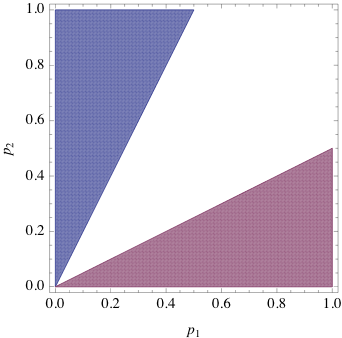
\includegraphics[width=2.2in]{Figure1a} & & 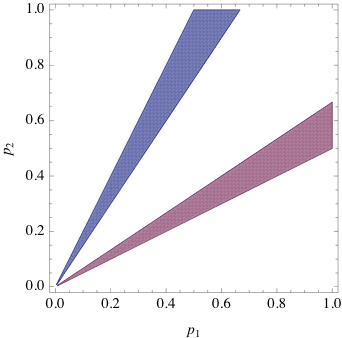
\includegraphics[width=2.2in]{Figure1b} \end{tabular}
 (c)
 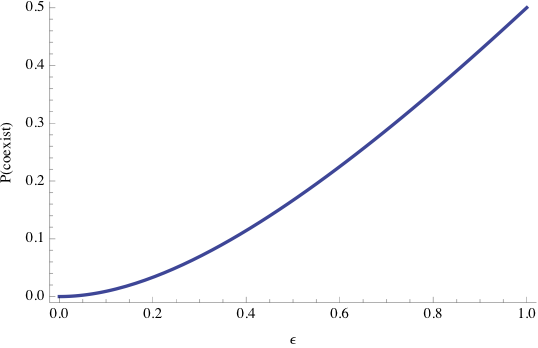
\includegraphics[width=4in]{Figure1c}
   \caption[Coexistence of two species with completely asymmetric competition]{\textbf{Coexistence of two species with completely asymmetric competition:} The regions of coexistence for two species are plotted in $p$-space. (a) shows the coexistence regions for $\epsilon=1$ while the case $\epsilon=1/2$ is shown in (b). Shaded regions in the upper left half of the plot are where both species coexist with growth rates $p_1<p_2$, or equivalently trait values $x_1>x_2$. The  regions to the bottom right of the plots represent the alternative ordering $p_1>p_2, x_1<x_2$. (c) shows how the probability of coexistence increases with the asymmetry parameter $\epsilon$, with large values indicating strong competitive asymmetry between individuals of different trait values.}
 \label{fig:2d}
\end{figure}

Since the trait values are limited to a finite range, it is possible to calculate the probability of coexistence for two species chosen at random from a uniform distribution on $x_1,x_2 \in [0,1]$  by calculating the size of the area within the unit box $[0,1]^2$ which satisfies \eqref{2dcond} as well as the assumption $x_1>x_2$. Here, we first find the area in $p-$space for which there exists an interior fixed point, and then from that calculate the area in $x-$space. Since $p$ is a decreasing function satisfying $p(0)=1, p(1)=0$, it is invertible with increasing inverse $p^{-1}$ that satisfies $p^{-1}(1)=0, \, p^{-1}(0)=1$, and hence the range of $p^{-1}$ is $[0,1]$. We first find the area in the $p_1,p_2$ plane, writing $p_i=p(x_i)$ for simplicity of notation, for which
\begin{equation}
\label{2dcond2}
\frac{p_2}{1+\epsilon}>p_1>p_2(1-\epsilon),\;\; (p_1,p_2)\in [0,1]^2,
\end{equation}
and then map this to an area in $x_1,x_2$ space.


Since the case $p(x_i)=1-x_i$ is linear and maps $[0,1]^2$ onto itself, the probability of coexistence is equal to the area of the $x-$space satisfying (\ref{2dcond}) which in turn equals the area in $p-$space satisfying \eqref{2dcond2}.

The areas satisfying these conditions for $\epsilon=1$ and $\epsilon=1/2$ are shown in Figure~\ref{fig:2d}. To calculate the size of the area in the $p_1,p_2$ plane where both equilibrium populations are greater than zero, we note that when \eqref{2dcond2} intersects the unit box, it forms a triangle $T$ with vertices $(0,0),(1-\epsilon,1)$ and $(1/(1+\epsilon),1)$. The area of $T$ in the $p_1,p_2$ plane is therefore given by
\[
\frac{1}{2}\left(\frac{1}{1+\epsilon}-(1-\epsilon)\right)=\frac{\epsilon^2}{2(1+\epsilon)},
\]
which is then multiplied by two to account for the other ordering of trait values $p_2<p_1$ (i.e. $x_2>x_1$) to give the area as
\[
A =\frac{\epsilon^2}{1+\epsilon}.
\]
This area is an increasing function in $\epsilon$, meaning that the greater the asymmetry observed in the competition between species, the more likely it is that two species can coexist together, as anticipated by our numerical simulations of the concave-convex function and analytical work on the piecewise linear function. Note that the result here is identical to that when $\Theta$ is small in the piecewise linear case.

 
\subsubsection{Communities with $n$-species}
In communities with $n>2$ species present,  any interior fixed point is unique and globally stable. While  \cite{nowak1994superinfection} state that this result holds with a modification of the theory in Chapter 21.3 of \cite{hofbauer1998evolutionary}, we include our own proof in Appendix~\ref{appendix1c}. 

In order to find the region of trait space that permits an interior fixed point, we consider the model written in the form
\begin{equation}
\frac{dN_i}{d\tau}=N_i\left(p_i(x) - \sum_{j=1}^n c_{ij}(x)N_j\right),
\end{equation}
where the $c_{ij}(x)$ competition coefficients combine to give the competition matrix $C(x)$. In Appendix~\ref{appendix1d}, we show that the volume of coexistence can be calculated from a determinant and is given explicitly by
\[
V_{n}=
\left\{
\begin{array}{rl}
\frac{\epsilon^{n}}{(1+\epsilon)^{n-1}} & \mbox{ even }n\geq 2\\
\frac{\epsilon^{n-1}}{(1+\epsilon)^{n-1}} & \mbox{ odd }n\geq 3. 
\end{array} \right.
\]
Therefore, for all $0<\epsilon \leq1$, it is possible for any number $n$ of species to coexist along a single competition-fecundity trade-off. However it is increasingly difficult for all species to coexist as the number of species in the environment increases, as shown by Figure~\ref{fig:ndif}.

\begin{figure}[htbp]
   \centering
   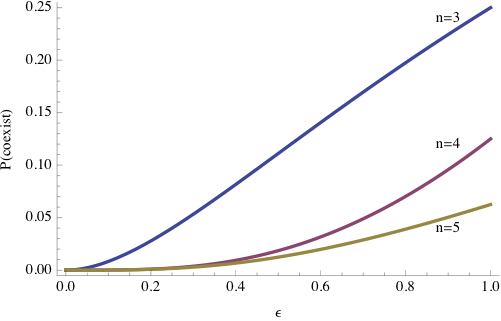
\includegraphics[width=4in]{Figure3}
   \caption[Change of probability of coexistence as number of species increases]{\textbf{Change of probability of coexistence as number of species increases:} How the probability of coexistence for different numbers $n$ of species decreases with $n$ is shown, along with how it changes with $\epsilon$, shown for $n=3,4,5$ species coexistence}
   \label{fig:ndif}
\end{figure}


\section{Discussion}

Life-history trade-offs have a rich history in helping to explain how competitors may coexist, but relatively few studies have quantified how rapidly the likelihood of coexistence declines with increasing number of species within the community. Here we have considered a trade-off between competitive ability and fecundity and have shown the probability of multiple species coexistence depends critically on the degree of asymmetry $\epsilon$ between them. Large values for $\epsilon$ indicate large competitive asymmetry between species with even nearby trait values, and it is here that coexistence is found to be most likely (see Figure~\ref{fig:ndif}). However, as the number of species drawn from the pool increases, even small decreases in the competitive asymmetry can lead to rapid declines in the likelihood of coexistence. The probability of sustaining at least two species also depends on the slope of the competition function at $c(z=0)$, and this is determined by the parameter $\Theta$. As $\Theta$ decreases, the steepness of the competition curve increases, and so does the probability of the trade-off maintaining multiple species. Therefore, maximum coexistence is likely to be achieved at high $\epsilon$ and low $\Theta$.

The trade-off considered here is essentially the same as the competition-colonisation trade-off, which has been much studied theoretically (e.g.  \cite{levin1974disturbance, hastings1980disturbance, tilman1994competition}) and empirically \citep[e.g.][]{turnbull1999seed, robinson1995invasibility, cadotte2007competition}. Although early theory suggested any number of species might be able to coexist on this trade-off \citep{may1994superinfection, tilman1994competition}, as we have shown here, coexistence is dependent upon the steepness of the trade-off function, and also on the amount of asymmetric competition between the species. Recent theory that builds on this trade-off has shown that high levels of coexistence are possible on a tolerance-fecundity trade-off, where species with seeds that can tolerate wide ranges in environmental conditions are assumed to be larger, and therefore fewer in number \citep{muller2010tolerance}. However, this still invokes strong competitive asymmetry because smaller seeded species are unable to germinate in environments outside of their tolerance zone, and it is probable that even some ability to germinate in non-preferred patches might greatly reduce the amount of coexistence that is possible.

Our results connect  to the results of \cite{adler2000space}, who showed the shape of the trade-off to be important for the number of species that can coexist; and with \cite{hillerislambers2003competition} who found strong trade-offs tend to enhance the coexistence of two species sharing one resource. We have extended this work to consider how rapidly the area for coexistence in trait-space diminishes with the number of species in the community. Our analyses reveal that even with the trade-off assumptions that most favour coexistence, the likelihood of coexistence diminishes very rapidly with the number of species, and this suggests relatively few species are ever likely to be able to coexist on one trade-off. Moreover, our results reveal that competitive asymmetry becomes more important in generating coexistence as the number of species increases (Figure~\ref{fig:ndif}; equation \eqref{nspecies}).

The methods we use are similar to those of \cite{meszena2006competitive} who calculated the likelihood of an interior fixed point existing and it's dependence on their model parameters. However, we note the existence of an interior fixed point is not sufficient for coexistence. For example, the symmetric May-Leonard model for three species \citep{may1975nonlinear}, always admits an interior equilibrium, yet the system only exhibits permanence when for each species, intraspecific competition is greater than twice the sum of the interspecific effects of the other two species. As such, their model represents an upper bound to the likelihood of coexistence. In the current paper, we address this by proving that the existence of an interior equilibrium is exactly equivalent to the permanence of the system, therefore adding to the conclusions made by Meszena et al.

Our results therefore show how important competitive asymmetry is in generating and maintaining large numbers of coexisting species; but how prevalent is competitive asymmetry in natural communities? There is a large body of work to suggest competitive asymmetry is common in animal \citep[e.g.][]{lawton1981asymmetrical, morin1988experimental,  resetarits1995competitive, costanzo2005asymmetrical} and plant communities \citep[e.g.][]{weiner1990asymmetric, connolly1996asymmetric, keddy1997experimental}. However, to our knowledge, except for seed size variation in plants \citep[e.g.][]{turnbull1999seed}, this competitive asymmetry has rarely been connected to a life-history trade-off. It is worth noting that many of these studies consider only two species, and the competition coefficients are often measured under one set of environmental conditions, so it is not clear how much this asymmetry extends into large communities of competitors, and whether there is a temporal fluctuation in the competitive hierarchy. One exception to this is a study by \cite{keddy1997experimental} who measured the competitive asymmetry between pairs of plant species drawn from a pool of 18 species. Their work concluded that in fact competitive asymmetry increased with soil productivity, and this is because light rather than soil nutrients became the limiting factor, and generally competition for light is expected to be size asymmetric, whereas competition for soil nutrients is usually size symmetric \citep[e.g.][]{weiner1990asymmetric}. 

The model we analyse here is biologically rather simple, and there is much scope for extensions that incorporate more realism. For example, as for most other models that study the competition-fecundity or competition-colonisation trade-offs, we assume that intraspecific competition is identical for all trait values (equation \eqref{rescaledmodel}); but it might be more realistic to assume that smaller individuals are better able to share resources than larger individuals, meaning the intraspecific competition term now has to be trait dependent as well.  We believe relaxing this assumption would yield rather more complex dynamics than the current model, including the possibility of founder control (i.e. unstable interior equilibria). For example,  \cite{calcagno2006coexistence} incorporated priority effects, whereby an adult plant cannot be displaced be a seed, into a competition-colonisation model, and showed that this can actually increase coexistence. However, when maximum colonisation rate, analogous to our maximum population growth rate, is heavily limited, such preemptive competition generally ceases to be beneficial to coexistence. Therefore,  this would reduce the amount of coexistence compared to that found here, and would place greater dependence on multiple trade-offs or other processes to generate coexistence between large numbers of species. 

The models presented here have assumed linear intrinsic growth rate $p$ in the absence of competition, and linear or piecewise constant competition for communities with three or more species. Nonlinearity, with suitable monotonicity conditions, can be easily incorporated into the function $p$, and the volume in $x-$space can then be found through a change of variable in the volume integral. Moreover, changing $p$ does not impact on the globally stability of interior steady states, which, as shown, depends solely on the competition matrix $C$. For models with three or more species, studying nonlinear competition functions gives the difficulty of not only finding volumes in space enclosed between curved surfaces, but also determining which points in these volumes are globally stable. The alternative, focusing on coexistence measured by permanence, also presents a serious challenge due to the lack of necessary and sufficient conditions for permanence in general competitive Lotka-Volterra models for $n>3$.

These extensions aside, we have shown here that competitive asymmetry could be very important in maintaining several species on a single trade-off; but that for large numbers of species multiple trade-offs; and/or other processes such as disturbance or natural enemies are required to maintain diverse competitive communities. Nonetheless, it is clear that competitive asymmetry which is widely observed in empirical studies could still interact with these other processes to increase, rather than decrease biodiversity as has often been supposed \citep[e.g.][]{keddy1997experimental, resetarits1995competitive}.

\section*{Acknowledgement}

Thanks to the reviewers for their comments. This work was funded by a Natural Environment Research Council (NERC) studentship to SN.

\section*{Appendices}
\bappendix
\section{Effect of the slope $c'(0)$ on coexistence}
\label{appendix1a}
We note that since $c(z)+c(-z)=2$ constant, we have that $c(-z)-1=1-c(z)>0$for positive $z$. Therefore, we can subtract \eqref{x2lower} from \eqref{x2upper} to get
\[
\frac{(1-z-c(z))-((1-z)c(-z)-1)}{c(-z)-1}=\frac{z(c(-z)-1)}{(c(-z)-1)}=z.
\]
Therefore the upper and lower bounds for $x_2$ coincide at $z=0$, and for $z>0$ the upper bound is always greater than the lower, i.e there is always a region where coexistence is possible. Therefore, if the upper bound \eqref{x2upper} is non-increasing, both it and the lower bound \eqref{x2lower} never exceed the value they achieve at $z=0$, and there is only a region of coexistence in the positive quadrant when the limit
\[
\lim_{z \to 0}\frac{1-z-c(z)}{1-c(z)} >0.
\]
As both numerator and denominator tend to zero, we use l'Hopital's rule to get that this limit is given by
\[
\frac{-1-c'(0)}{-c'(0)}
\]
which is positive for $c'(0)<-1$.

It remains to demonstrate that \eqref{x2upper} is non-increasing for positive $z$. The derivative of the function is given by
\[
\frac{c(z)-1-zc'(z)}{(1-c(z))^2}.
\]
If $c'(z)=0$, then this becomes
\[
\frac{-1}{1-c(z)}<0, \]
since $c(z)<1$ for all $z>0$. When $c'(z)<0$, then we note that the function is non-increasing for 
\[
z\leq \frac{c(z)-1}{c'(z)}.
\]
The derivative of the right hand side is given by
\[
1-\frac{c''(z)(c(z)-1)}{c'(z)^2}
\]
which is greater than one for all positive $z$. Therefore, this point increases faster than $z$. Noting that the derivative of \eqref{x2upper} is zero when $z=0$, we can therefore conclude that for all $z>0$, this upper bound is indeed non-increasing.

\section{The absence of asymmetry}
\label{appendix1b}
Without losing any generality, we can order traits such that $x_1>x_2 > \cdots > x_n$ so that since $p$ is decreasing, $p(x_1)< p(x_2) < \cdots < p(x_n)$. When $\epsilon=0$, equations \eqref{rescaledmodel} become
\[
\frac{d N_i}{d\tau}=N_i\left(p(x_i)-\sum_{j=1}^n N_{j}\right), \;\; i=1,\ldots,n.
\]
Thus if $i < k$,
\[
\frac{d}{d\tau} \log (N_i/N_k) = p(x_i)-p(x_k)<0.
\]
This shows that for $i<k$
\[
N_i(\tau) = N_k(\tau) e^{( p(x_i)-p(x_k)) \tau} \rightarrow 0, \;\; \tau\rightarrow \infty
\]
since $N(t)$ is bounded. This shows that $N_{i}(\tau)\rightarrow 0$ as $\tau\rightarrow \infty$ for $i=1,2,\ldots,n-1$. It is intuitive that the remaining species density $N_n(\tau) \rightarrow p(x_n)$ as $\tau\rightarrow \infty$. This can be shown by first noting that the equation for the dynamic of $N_n$ reduces to  the time-dependent logistic equation:
\begin{equation}
\dot{N}_n = p(x_n) N_n \left(1-\frac{N_n}{K(t)}\right), \label{ss1}
\end{equation}
where the time-dependent carrying capacity is given by 
\[
K(t) = p(x_n)e^{p(x_n)t}/(\sum_{i=1}^n e^{p(x_i)t}).
\] One may verify that the explicit solution to (\ref{ss1}) is
\[
N_n(t) = \frac{N_n(0) e^{p(x_n)t}}{1+N_n(0)\sum_{i=1}^n \left( \frac{e^{p(x_i)t}-1}{p(x_i)} \right)}\rightarrow p(x_n)\mbox{ as } t\rightarrow \infty.
\]
We have thus shown that the species with minimum trait $0$ will send any other species to extinction.

\section{Global Stability of interior fixed points}
\label{appendix1c}
\begin{lem}Whenever an interior fixed point exists for the $n$-species model given by \eqref{rescaledmodel}, it is both unique and globally asymptotically stable relative to the interior of the region of space where all $N_i$ are positive, and therefore the system displays permanence.\end{lem}
\begin{proof} It is well known that when \eqref{model} admits an interior steady state, it is globally stable (also known as LV-stable) if the  matrix $-C=((-c_{ij}(x)))$ is dissipative, that is, there exists a positive diagonal matrix $D$ such that the real symmetric matrix $D(-C)+(-C)^TD$ is negative definite, and therefore has only negative eigenvalues \citep[e.g.][]{hofandsig}. For the model with discontinuous competition,  the competition matrix takes the form (in the region $x_1>x_2>\cdots > x_n$) given by equation \eqref{constant_C}. 
Let $D$ be a positive diagonal matrix with diagonal entries $\theta_i$ ($i=1,\ldots,n$).
Then \eqref{model}, with competition matrix $C$ as in \eqref{constant_C}, admits a  fixed point that globally attracts interior trajectories whenever the real symmetric matrix $A=(DC+C^TD)$, given by
\[
\label{posdef}
\begin{pmatrix}
2\theta_1&(1-\epsilon)\theta_1+(1+\epsilon)\theta_2&\cdots&(1-\epsilon)\theta_1+(1+\epsilon)\theta_n\\
(1-\epsilon)\theta_1+(1+\epsilon)\theta_2&2\theta_2& \cdots&(1-\epsilon)\theta_2+(1+\epsilon)\theta_n\\
(1-\epsilon)\theta_1+(1+\epsilon)\theta_3&(1-\epsilon)\theta_2+(1+\epsilon)\theta_3&\cdots&(1-\epsilon)\theta_3+(1+\epsilon)\theta_n\\
\vdots&\vdots&\ddots&\vdots&\\
(1-\epsilon)\theta_1+(1+\epsilon)\theta_n&(1-\epsilon)\theta_2+(1+\epsilon)\theta_n&\cdots&2\theta_n
\end{pmatrix} 
\]
has all positive eigenvalues, which is the case if all the leading principal minors are positive.

We have fixed $\theta_i>0$ positive, so we restrict ourselves to looking at $m\times m$ leading principal minors of the matrix $A$ with $m\geq2$:
\[
 \begin{vmatrix}
2\theta_1 & (1-\epsilon)\theta_1+(1+\epsilon)\theta_2 & \cdots & (1-\epsilon)\theta_1+(1+\epsilon)\theta_m \\
(1-\epsilon)\theta_1+(1+\epsilon)\theta_2 & 2\theta_2 &\cdots & (1-\epsilon)\theta_2+(1+\epsilon)\theta_m \\
\vdots&\vdots&\ddots&\vdots \\
(1-\epsilon)\theta_1+(1+\epsilon)\theta_m & (1-\epsilon)\theta_2+(1+\epsilon)\theta_m &\cdots & 2\theta_m \end{vmatrix}. 
\]
As the determinant of a matrix is not changed when one row or column is subtracted from another, we then subtract the $(m-1)$th column from the $m$th column, and the $i$th column from the $(i+1)$th column for all $1\leq i\leq m-1$ to obtain the matrix
\[
 \begin{vmatrix}
2\theta_1 &(1+\epsilon)(\theta_2-\theta_1) & \cdots &(1+\epsilon)(\theta_m-\theta_{m-1}) \\
(1-\epsilon)\theta_1+(1+\epsilon)\theta_2 & (1-\epsilon)(\theta_2-\theta_1) &\cdots & (1+\epsilon)(\theta_m-\theta_{m-1}) \\
\vdots&\vdots&\ddots&\vdots \\
(1-\epsilon)\theta_1+(1+\epsilon)\theta_m & (1-\epsilon)(\theta_2-\theta_1) &\cdots & (1-\epsilon)(\theta_m-\theta_{m-1}) \end{vmatrix}. 
\]
Removing the common factors in columns 2 up to $m$ give that the determinant has a factor
\[
(-1)^{m-1}\prod_{i=1}^{m-1}(\theta_i-\theta_{i+1})
\]
which is then multiplied by
\[
\begin{vmatrix}
2\theta_1 & 1+\epsilon & 1+\epsilon & \cdots & 1+\epsilon \\
(1-\epsilon)\theta_1+(1+\epsilon)\theta_2&1-\epsilon&1+\epsilon&\cdots&1+\epsilon \\
(1-\epsilon)\theta_1+(1+\epsilon)\theta_3&1-\epsilon&1-\epsilon&\cdots&1+\epsilon \\
\vdots&\vdots&\vdots&\ddots&\vdots \\
(1-\epsilon)\theta_1+(1+\epsilon)\theta_m&1-\epsilon&1-\epsilon&\cdots&1-\epsilon \end{vmatrix}.
\]
Subtracting row $m-1$ from row $m$, and row $i$ from row $i+1$ for all $i<m$ gives this determinant as
\begin{align}
&\begin{vmatrix}
2\theta_1 & 1+\epsilon&1+\epsilon&\cdots&1+\epsilon \\
(1+\epsilon)(\theta_2-\theta_1)&-2\epsilon&0&\cdots&0 \\
(1+\epsilon)(\theta_3-\theta_2)&0&-2\epsilon&\cdots&0 \\
\vdots&\vdots&\vdots&\ddots&\vdots \\
(1+\epsilon)(\theta_m-\theta_{m-1})&0&0&\cdots&-2\epsilon \end{vmatrix} \notag \\
=&\begin{vmatrix}
2\theta_1&1+\epsilon&0& 0&\cdots&0\\
(1+\epsilon)(\theta_2-\theta_1)&-2\epsilon&2\epsilon &0&\cdots&0\\
(1+\epsilon)(\theta_3-\theta_2)&0&-2\epsilon&2\epsilon&\cdots&0\\
\vdots&\vdots&\vdots&\vdots&\ddots&\vdots \\
(1+\epsilon)(\theta_m-\theta_{m-1})&0&0&0&\cdots&-2\epsilon\end{vmatrix}\notag \\
=&(-1)^{m-1}\theta_12^m\epsilon^{m-1} - (1+\epsilon)^2(2\epsilon)^{m-2}(-1)^{m-2}\left(\theta_2-\theta_1+\theta_3-\theta_2+\dots+\theta_m-\theta_{m-1}\right)\notag \\
=&(-1)^{m}(2\epsilon)^{m-2}\left( (1-\epsilon)^2\theta_1-(1+\epsilon)^2\theta_m\right). \notag
\end{align}
Therefore, the $m\times m$ leading principal minor for $m>1$ is given by
\begin{equation}
-(2\epsilon)^{m-2}\left( (1-\epsilon)^2\theta_1-(1+\epsilon)^2\theta_m\right)\prod_{i=1}^{m-1}(\theta_i-\theta_{i+1}). \label{baig1}
\end{equation}
It remains to be shown that the $\theta_i$ can be chosen such that all leading principal minors (\ref{baig1}) are positive, which is the case when $\left( (1-\epsilon)^2\theta_i-(1+\epsilon)^2\theta_j\right)<0$ and $(\theta_i-\theta_j)>0$ for $i<j$. Setting
\[
\theta_i=n-\frac{1}{(1+\epsilon)^{n+1-i}}
\]
then we can use $j-i\geq1$ to calculate that
\begin{align}
\theta_i-\theta_j=&\left(n-\frac{1}{(1+\epsilon)^{n+1-i}}\right)-\left(n-\frac{1}{(1+\epsilon)^{n+1-j}}\right) \notag \\
=&\frac{(1+\epsilon)^{j-i}-1}{(1+\epsilon)^{n+1-i}} \notag \\
\geq&\frac{1+\epsilon - 1}{(1+\epsilon)^{n+1-i}}>0. \notag
\end{align}
To show that $\left( (1-\epsilon)^2\theta_i-(1+\epsilon)^2\theta_j\right)<0$ we note that
\begin{align*}
\left( (1-\epsilon)^2\theta_i-(1+\epsilon)^2\theta_j\right)&<\left( (1-\epsilon)^2\theta_1-(1+\epsilon)^2\theta_j\right)\\
&<\left( (1-\epsilon)^2\theta_1-(1+\epsilon)^2\theta_n\right)
\end{align*}
and that for $\epsilon=0$, we have $\left( (1-\epsilon)^2\theta_1-(1+\epsilon)^2\theta_n\right)=0$. Differentiating this with respect to epsilon gives
\begin{align*}
\frac{d}{d\epsilon}\left( (1-\epsilon)^2\theta_i-(1+\epsilon)^2\theta_j\right)&=-4n+1+2\frac{1-\epsilon}{(1+\epsilon)^n}+n\frac{(1-\epsilon)^2}{(1+\epsilon)^{n+1}}\\
&\leq-4n +1+2+n < 0
\end{align*}
for all $0\leq \epsilon \leq 1$ and $n\geq2$. Therefore, since $\epsilon=0$ is a root for the function, for any $\epsilon>0$, we have
$$\left( (1-\epsilon)^2\theta_1-(1+\epsilon)^2\theta_n\right)<0$$
and therefore
$$\left( (1-\epsilon)^2\theta_i-(1+\epsilon)^2\theta_j\right)<0.$$
Therefore, all the leading principal minors are positive, meaning that $A=DC+C^TD$ is positive definite. Therefore $D(-C)+(-C)^TD$ is negative definite, as required for global stability. Global stability immediately implies permanence. \begin{flushright} $\square$ \end{flushright}
 \end{proof}
 
 \section{Size of the coexistence region}
 \label{appendix1d}
Here we calculate the probability of coexistence for an $n$ species version of \eqref{rescaledmodel}. Since we are using the step function \eqref{stepc}, the matrix $C(x)$ is piecewise constant. At the interior fixed point the bracketed terms are equal to zero, which therefore reduces the model to
$
\mathbf{p}(x)=C(x)\mathbf{N},
$
with $\mathbf{p}$ the vector of the growth rate of each species and $\mathbf{N}$ the vector with $i$th component $N_i$. Since $C(x)$ is non-singular, this is the rearranged to give the solution 
$
\mathbf{N}=C^{-1}(x)\mathbf{p}(x)$. 
We are interested in the volume of $x$-space for which $\mathbf{N}=C^{-1}(x)\mathbf{p}(x)> \mathbf{0}$. To find this volume, we find the volume in $p$-space where $p_1 < p_2 <\cdots < p_n$ which satisfies, since then $x_1>x_2> \cdots > x_n$ and so $C(x)$ is a constant, and non-singular matrix $C$, so that
\begin{equation}
C^{-1}\mathbf{p} = \mathbf{0}. \label{planes1}
\end{equation}
Equation \eqref{planes1} defines a series of planes in $p-$space that all pass through the origin. When an ordering $p_n>p_{n-1}>\dots>p_1$ is assumed without any loss of generality, these planes form an $n$ dimensional pyramid when intersected with the unit cube. The volume of this pyramid is then the probability of the $n$ species model permitting an interior fixed point, and therefore the probability of all $n$ species coexisting due to the stability result in Appendix~\ref{appendix1c}.

With the ordering $p_1<p_2<\dots<p_n$, equivalent to $x_1>x_2>\dots>x_n$, the competition matrix $C$ takes the form
\begin{equation}
\label{constant_C}
C=\begin{pmatrix}
1 & 1-\epsilon &1-\epsilon & \cdots & 1-\epsilon \\
1+\epsilon&1&1-\epsilon&\cdots&1-\epsilon \\
1+\epsilon&1+\epsilon&1&\cdots&1-\epsilon \\
\vdots&\vdots&\vdots&\ddots&\vdots \\
1+\epsilon&1+\epsilon&1+\epsilon&\cdots&1 \end{pmatrix}.
\end{equation}
It is relatively simple to show that $C$ is non-singular, allowing us to calculate the volume of the $n$ dimensional pyramid. We need to find the $n$ points at which $n$ of the planes intersect the face $p_n=1$. To find these points, we note that the edges of the $n$ dimensional pyramid must be orthogonal to each of the $n-1$  planes in $p-$space defined by \eqref{planes1} that meet at that edge. Since $C^{-1}C=I_n$, each column of $C$ is orthogonal to all bar one of the rows of $C^{-1}$ Therefore, the edges of the $n$ dimensional pyramid point in the direction of the columns of $C$. These edges meet the plane $p_n=1$ at the non-zero corners of the $n$ dimensional simplex, so it is simple to show that these points are given by the columns of $C$, scaled such that the value of $p_n=1$. Therefore, the $n$ non-zero vertices of the  simplex that lie in the plane $p_n=1$ are given by
\begin{gather*}
\left(\frac{1}{1+\epsilon},1,1,1,\dots, 1\right), \\
\left(\frac{1-\epsilon}{1+\epsilon}, \frac{1}{1+\epsilon}, 1, 1,\cdots, 1\right), \\
\left(\frac{1-\epsilon}{1+\epsilon}, \frac{1-\epsilon}{1+\epsilon},\frac{1}{1+\epsilon}, 1,\cdots, 1\right), \\
\vdots \\
\left(\frac{1-\epsilon}{1+\epsilon}, \frac{1-\epsilon}{1+\epsilon},\frac{1-\epsilon}{1+\epsilon},\cdots, \frac{1}{1+\epsilon},1\right), \\
\left(1-\epsilon, 1-\epsilon,1-\epsilon,\cdots, 1-\epsilon,1\right).
\end{gather*}
\begin{thm} the  probability of coexistence, is given by
\begin{equation}
\label{nspecies}
V_n=P(\text{coexist}_n)=\begin{cases}
\frac{\epsilon^n}{(1+\epsilon)^{n-1}} &  \mbox{ even }n\geq 2 \\
\frac{\epsilon^{n-1}}{(1+\epsilon)^{n-1}} &   \mbox{ odd }n\geq 3 \end{cases}.
\end{equation} \end{thm}
\begin{proof}
The volume of the $n$ dimensional simplex  is given by 
\[
\bar{V}_n=\frac{1}{n!}\begin{vmatrix}
\frac{1}{1+\epsilon}&1&1&1&\cdots &1&1\\
\frac{1-\epsilon}{1+\epsilon} & \frac{1}{1+\epsilon} & 1& 1& \cdots &1&1\\
\frac{1-\epsilon}{1+\epsilon} & \frac{1-\epsilon}{1+\epsilon}& \frac{1}{1+\epsilon} & 1& \cdots &1&1\\
\vdots&\vdots&\vdots&\vdots&\ddots&\vdots\\
\frac{1-\epsilon}{1+\epsilon} & \frac{1-\epsilon}{1+\epsilon}& \frac{1-\epsilon}{1+\epsilon} & \frac{1-\epsilon}{1+\epsilon}& \cdots &\frac{1}{1+\epsilon}& 1\\
1-\epsilon & 1-\epsilon & 1-\epsilon & 1-\epsilon& \cdots & 1-\epsilon & 1
 \end{vmatrix}.
\]
Since there are $n!$ of these volumes, one for each ordering of the traits, so the total volume is $V_{n} = n! \bar{V}_n$. Let $U_n = n! (1+\epsilon)^{n-1}\bar{V}_n$. Then 
\[
U_n=\begin{vmatrix}
1&1+\epsilon&1+\epsilon&1+\epsilon&\cdots &1+\epsilon&1+\epsilon\\
1-\epsilon& 1 & 1+\epsilon& 1+\epsilon& \cdots &1+\epsilon&1+\epsilon\\
1-\epsilon &1-\epsilon&1 & 1+\epsilon& \cdots &1+\epsilon&1+\epsilon\\
\vdots&\vdots&\vdots&\vdots&\ddots&\vdots\\
1-\epsilon&1-\epsilon&1-\epsilon&1-\epsilon& \cdots &1& 1+\epsilon\\
1-\epsilon& 1-\epsilon &1-\epsilon &1-\epsilon& \cdots &1-\epsilon& 1
 \end{vmatrix}.
\]
We now show that $U_n = \epsilon^2  U_{n-2}$. To see this, first subtract the second row from the first row. Having done this, in the new determinant subtract the first column from the second column. This gives
 \[
U_n=\begin{vmatrix}
\epsilon & 0 &0&0&\cdots &0&0\\
1-\epsilon& \epsilon & 1+\epsilon& 1+\epsilon& \cdots &1+\epsilon&1+\epsilon\\
1-\epsilon &0&1 & 1+\epsilon& \cdots &1+\epsilon&1+\epsilon\\
\vdots&\vdots&\vdots&\vdots&\ddots&\vdots\\
1-\epsilon&0&1-\epsilon&1-\epsilon& \cdots &1& 1+\epsilon\\
1-\epsilon& 0 &1-\epsilon &1-\epsilon& \cdots &1-\epsilon& 1
 \end{vmatrix},
\]
which gives $U_n = \epsilon^2 U_{n-2}$ as required. Now quick calculations show that $U_2=\epsilon^2$ and $ U_3 = \epsilon^2$ so that $U_n = \epsilon^n$ for $n\geq 2$ even and $ U_n = \epsilon^{n-1}$ for $n\geq 3$ odd.
 \begin{eqnarray*}
\bar{V}_{n} &=& \frac{1}{n!} \frac{\epsilon^n}{(1+\epsilon)^{n-1}} \mbox{ $n$ even}\\
 &=&\frac{1}{n!}\frac{\epsilon^{n-1}}{(1+\epsilon)^{n-1}} \mbox{ $n$ odd.}
 \end{eqnarray*}

\[
V_{n}=
\left\{
\begin{array}{rl}
\frac{\epsilon^{n}}{(1+\epsilon)^{n-1}} & \mbox{ even }n\geq 2\\
\frac{\epsilon^{n-1}}{(1+\epsilon)^{n-1}} & \mbox{ odd }n\geq 3. 
\end{array} \right.
\]   
\end{proof}

\eappendix


\newpage
\chapter{The effect of disturbance intensity and frequency on coexistence via a fecundity-growth trade-off}
\newpage
\topskip0pt
\vspace*{\fill}
\section*{Abstract}
Disturbance has been suggested as an important promotor of species coexistence, and the intermediate disturbance hypothesis (IDH) suggests that diversity should be maximised at intermediate levels of disturbance. However, the mechanism by which disturbance is increased is often not explicitly stated in studies, or is a composite measure containing many different aspects of disturbance. We use a stochastic lottery-type model to demonstrate that among species competing for light along a fecundity-juvenile growth trade-off, a) disturbance can increase or decrease diversity;  b) the aspect of disturbance (intensity or frequency) that is measured can make a dramatic difference to the qualitative results obtained; and these results are robust to changes in system capacity (the number of individuals the system is capable of maintaining), and also productivity.
\vspace*{\fill}
% \PACS{PACS code1 \and PACS code2 \and more}
% \subclass{MSC code1 \and MSC code2 \and more}
\newpage
\section{Introduction}
\label{intro}
One of the most persistent issues in ecology is how some communities, such as tropical forests, grasslands and coral reefs maintain high levels of species diversity. Some mechanisms such as resource partitioning \citep[e.g.][]{sala1989resource,schoener1974resource} and the storage effect \citep{warner1985coexistence} are widely recognised, while several previous studies \citep[e.g.][]{denslow1987tropical,sousa1984role} have suggested that disturbance events may play an important part in promoting diversity in some systems. Disturbance, that is, an event that results in the death of large number of individuals and alter niche opportunities \citep{shea2004moving}, creates an environment that prevents the exclusion of weaker competing species, such as pioneer species. If levels of disturbance are too low, these pioneer-like species will be excluded, whereas if disturbance levels are too high they will drive strong competitors with slow recruitment, for example late successional tree species, to extinction. Thus only at intermediate disturbance levels is it possible for both early- and late- successional species to coexist. It is on these arguments that the intermediate disturbance hypothesis (IDH) suggests that intermediate levels of disturbance allow the maximal level of species diversity \citep[e.g.][]{connell1978diversity,huston1979general}, producing a peaked diversity-disturbance relationship (DDR).

The IDH was proposed to address the specific issue of tree diversity in tropical forests and fish and coral diversity in coral reefs \citep{connell1978diversity}, but can also be traced back to \cite{grime1973competitive}. Despite this long history, the fact that disturbances often occur infrequently, and because in many communities individuals may be relatively long-lived, means it has been hard to test the IDH and empirical studies have shown mixed results \citep[see review in ][]{mackey2001diversity}. Some support for the IDH has been found \citep[e.g.][]{biswas2010disturbance,molino2001tree,rogers1993hurricanes} while other studies reject the hypothesis \citep[e.g.][]{hubbell1999light,huxham2000field}. \cite{bongers2009intermediate} find that diversity does indeed peak at intermediate disturbance levels, but they also conclude that disturbance does not contribute much to diversity, especially in wet or moist forests.

It has been argued that there are at least three different axes upon which disturbances should be measured: frequency; area affected; and intensity \citep{malanson1984intensity,miller1982community,sousa1984role}.  However, many empirical studies consider disturbance levels in forests as a single parameter, such as the total area lost in a given time period (effectively frequency multiplied by intensity) \citep[e.g.][]{molino2001tree,nakagawa2000impact,peterson1997tornado}. Fire ecology studies have often acknowledged the difference between different factors influencing fire, such as ignition probability and spread \citep[e.g.][]{kilgore1979fire,turner1994landscape}, observing that most fires are of low intensity and high frequency \citep{kilgore1979fire}, while spatial connectedness has an impact on overall fire intensity \citep{turner1994landscape}. However, there remain relatively few theoretical studies that consider the relative impact of frequency and intensity of disturbances \citep[but see ][]{miller2011frequency}. In an early review of the empirical literature, \cite{denslow1980patterns} indicated that communities that have infrequent but large patches cleared through disturbance can be more diverse than those that suffer frequent, but small-scale disturbances (e.g. gaps created by tree-fall). \cite{hartshorn1978treefalls} reported that in a Costa Rican forest most disturbances are caused by relatively small gaps appearing after a tree falls and that as a consequence the forest is dominated by shade-tolerant species. In a recent theoretical study, \cite{miller2011frequency} show how disturbance intensity and frequency have different effects on community dynamics and the emergence of the IDH depends greatly on the combination of the two. It seems likely that this may be a significant factor behind the relative lack of consensus on whether or not the classical IDH pattern is general in nature communities.

Productivity of a system is also known to have a significant effect on disturbance; \cite{kondoh2001unifying} used the dynamic equilibrium model of \cite{huston1979general} to demonstrate theoretically that an increase in productivity leads to an increase the disturbance levels that give peak diversity. This is supported by empirical evidence as reviewed by \cite{proulx1998reversal}, who report that species richness increases with disturbance in nutrient-rich environment, but decreases in environments where nutrients are scarce. Both the theoretical and empirical results suggest that the nature of a communities response to disturbance can be affected by the level of productivity. \cite{kondoh2001unifying} suggests these results are due to contrasting effects of disturbance and productivity; where disturbance favours the stronger coloniser by creating more empty sites, productivity increases work to reduce the advantage of strong colonisers by increasing the colonisation rate of all species.

Here we build on this work and consider the effects of disturbance frequency and intensity separately in a two species forest model, in which there is a fecundity-growth trade-off with system capacity, the number of individuals the community can support at saturation, as a parameter. Analyses of the model confirm that the frequency and intensity of the disturbance can have significantly different effects, and that the emergence of the IDH is dependent upon the combination of disturbance intensity and frequency. We also demonstrate that thee results are robust to changes in system capacity and productivity.

\section{The Model}
\label{model}
We consider a simple lottery type model, originally introduced by \cite{sale1978coexistence} and \cite{chesson1981environmental} and used extensively since \citep[e.g.][]{muko2000species,pacala1992herbivores}. There are a fixed number $N$ distinct sites, each capable of supporting a single adult individual, observed in continuous time $\tau$. At discrete times $\tau_1,\tau_2, \dots$, there is a tree death, selected at random from the community, followed by competition between the remaining individuals for the vacated site. We assume that the time to fill a gap with an individual is small enough that the gap created at time $\tau_t$ is filled by an adult individual by time $\tau_{t+1}$, i.e. death-replacement events are sufficiently far apart temporally that they do not overlap and can be considered as discrete events. This assumption makes it possible to model this system as a time homogeneous Markov Chain (MC) model. With the range of parameters considered below, the expected gap replenishment time is approximately 4 years. Simulations reducing the number of adult trees by 4\% (consistent with 1\% annual mortality for this replenishment period) do not exhibit any qualitative difference.

Gaps are occupied by populations of two species $N_1(t), N_2(t)$, such that $N_1(t) + N_2(t) = N$, where $t$ represents time as measured by the number of replacement events that have occurred, i.e. $N_i(t)$ represents the population of species $i$ after the gap created at time $\tau_t$ has been filled, and before another gap is created at time $\tau_{t+1}$. Because after each death-replacement event, the number of individuals is fixed, we consider the dynamics of species 1 only, modelling $N_1(t)=n$ with $N_2(t)=N-n$. We assume 
\begin{enumerate}
\item The system is closed, so no seeds are introduced from elsewhere. Biologically, this could suggest an island population or community isolated by other geographic constraints. A low level of immigrating seeds does not qualitatively affect the results.
\item The individuals considered are asexual or self-fertilising, so that a single individual can produce seeds, and that individuals are always reproductively active.
\item The two species differ only in growth rates $g_i$ and annual per capita seed production $s_i$, with a trade-off between competitive ability (growth) and colonisation ability (seed numbers). Species 2 has the higher growth rate of the two species, $g_2>g_1$, while species 1 is the more fecund $s_1>s_2$. Note that if this trade-off is relaxed, such that $s_2\geq s_1$, coexistence is impossible, with species 2 dominating. We note that species 2 is in effect seed limited as it would win more sites if it were able to send seeds there; whereas species 1 is competitor limited and would gain proportionally more sites if species 2 were rare.
\item As individuals compete for light in a gap, we assume complete asymmetric competition. Once the combined size of the juveniles in a gap is that of a single adult, then the largest individual will win the site. Competition for a site is therefore a race to reach size $C/2$, where $C$ is the size of an adult individual.
\item It is possible for the faster growing species 2 to usurp juveniles of the slower growing species. The initial juvenile to reach a gap is determined by lottery, but species 2 may take over the site if further seeds arrive before a species 1 juvenile has grown sufficiently large. To usurp species 1, species 2 requires seeds to arrive before species 1 has been present for time $x=C(1/g_2-1/g_1)/2$.
\item Seeds are all assumed to be viable and are dispersed at random in the environment by a homogeneous Poisson process (with rate $\lambda_i =s_iN_i(t)/N$) as per high distance dispersals in \cite{clark1999interpreting}.
\item Disturbance events occur at each time step with probability $f=(dNT_D)^{-1}$ where $T_D$ is the expected number of years between disturbance events, and $d$ is the expected annual mortality rate (fixed at $1\%$). Within these events, individuals die with probability $I$ (the intensity of the disturbance), before the remaining individuals compete to fill the emptied sites. Increasing either frequency $f$ or intensity $I$ will result in an increase in total basal area lost over a given time frame, a standard measure of disturbance \citep[e.g.][]{molino2001tree,peterson1997tornado}.
\end{enumerate}
When a disturbance does not occur (with probability $1-f$), the number of species 1 individuals will increase if a species 2 individual dies, seeds from species 1 reach the site first, and then grow for time $x$ without species 2 reaching the site. As both species have the same dispersal kernel, this gives
\begin{align}
\label{increase}
P(\text{Increase}(n))&=P(N_1(1)=n+1)|N_1(0)=n) \\
&=\frac{N-n}{N}\frac{s_1 n}{s_1 n +s_2(N-n-1)}\exp \left( -s_2 \frac{N-n-1}{N} x\right),\notag \end{align}
where the exponential term is the probability that no species 2 seeds arrive in time $x$. Similarly, species 1 will decline in numbers if it suffers a death, and species 2 claims the site, either arriving at the site first or by successfully invading a site where species 1 juveniles are present, giving
\begin{align}
\label{decrease}
P(\text{Decrease}(n))=&P(N_1(1)=n-1 | N_1(0)=n)  \\ 
=&\frac{n}{N}\frac{s_2 (N-n)}{s_1 (n-1) +s_2(N-n)} \notag \\
& + \frac{n}{N}\frac{s_1 (n-1)}{s_1 (n-1) +s_2(N-n)}\left(1-\exp \left( -s_2 \frac{N-n}{N} x\right)\right). \notag \end{align}
All other possibilities result in the populations of the two species remaining the same after a time step, so we use a third function $P(\text{Stay}(n))=1-P(\text{Increase}(n))-P(\text{Decrease}(n))$ to fully define the transition probabilities, giving a $(N+1) \times (N+1)$ tridiagonal transition matrix $A$, with $A_{i,i}=P(\text{Stay}(i-1)), A_{i,i+1}=P(\text{Increase}(i-1)), A_{i,i-1}=P(\text{Decrease}(i-1))$.

During a disturbance event, each individual has a probability $I$ of mortality, resulting in $d_{dist}=d_1+d_2$ total deaths, where $d_i$ is the number of species $i$ deaths. The remaining $N-d_{dist}$ individuals compete over the empty site, with species 1 colonising if it reaches the site at least time $x$ before species 2. Therefore, species 1 will take a site with a probability defined by the function
\begin{equation}
\label{sp1}
Sp_1(n_1^*,n_2^*)=\frac{s_1 n_1^*}{s_1n_1^*+s_2n_2^*}\exp \left(-s_2 x\frac{n_2^*}{N}\right),
\end{equation}
where $n_1^*,n_2^*$ are the populations remaining immediately after the deaths from a disturbance event.

In the results below, we also relax assumption 2 listed above; that each individual is reproductively active all the time, which has the effect of reducing the productivity of the system. Instead, each time a gap is contested, we suppose that each individual is producing seeds with probability $p$. This parameter $p$ is assumed to be time invariant and independent of species abundance, as well as constant across species. This allows us to consider the effects of seed limitation, which we compare with other ways of altering productivity.


A standard tool for measuring coexistence in a stochastic model is to find an everywhere positive and steady probability distribution. Such a steady distribution is ecologically relevant only if it is stable. However, in the case where the model has absorbing boundaries, and the probability of reaching those boundaries is greater than zero, the only steady state distributions are those absorbing boundaries, where a species exists in monoculture. 

Since the model is stochastic, and the boundaries are absorbing, the long-term expectation is for a monoculture where one or other species goes extinct. Of course, it may take a long time to reach these boundaries. We therefore consider a variant of invasion analysis, similar to that introduced by \cite{chesson1989invasibility} and \cite{ellner1989convergence}. \cite{chesson1982stabilizing} proved that when the boundary growth rates, or average changes at the boundaries are positive, such that each species will on average increase when rare, the populations are stochastically bounded away from zero, and coexistence is expected. Note that because the model presented here uses a discrete state space, the invasion criteria are considered with a single individual of the invader present, as opposed to being assessed at 0 as in a continuous state space (we are modelling individuals, not densities or proportions of sites occupied). We approximate the expected change at the boundaries ($n=1,N-1$) using the formula
\begin{equation}
\label{avchange}
\begin{array}{rl}
\text{AverageChange}(n) = (1-f)\left[P(\text{Increase}(n))-P(\text{Decrease}(n))\right]&\\[0.75em]
+ f\left[ NI Sp_1(n(1-I)) - nI\right]&.
\end{array}
\end{equation}
The first term in \eqref{avchange} is the expected change when disturbance does not occur multiplied by the within-event probability that there is no disturbance event. The second term indicates the expected change during a disturbance as measured by the expected remaining populations. Due to Jensen's inequality, this is not the actual expected change, but an approximation. This approximation improves as system capacity $N$ is increased, as demonstrated in Appendix~\ref{app2a}, and works well for $N\geq500$. Coexistence is predicted for regions of parameter space where the following 2 inequalities both hold;
\begin{align}
\label{ac1}\text{AverageChange}(1)&>0, \\
\label{acn-1}\text{AverageChange}(N-1)&<0. \end{align}
Note that when there is no disturbance ($T_D=\infty$), these conditions simplify to 
\begin{align}
\label{lowerboundarycond}P(\text{Increase}(1))&>P(\text{Decrease}(1)) \\
\label{upperboundarycond}P(\text{Increase}(N-1))&<P(\text{Decrease}(N-1)). \end{align}
In biological terms, these conditions can be considered as the following: If there is a single individual of a species remaining, for that species to persist it must produce offspring that successfully colonise at least one other site before the adult dies. We implicitly assume that either individuals are asexual, or that self-fertilisation is possible, and more complex models are required to investigate sexual populations that are self-incompatible. The colonisation of a second site therefore must be more likely than the death of this single individual. Analyses using these conditions are extensively checked against time series simulations.

\section{Results} \label{results}
\subsection{Coexistence without disturbances ($T_D=\infty$)}
\label{ss:resultshomo}

Substituting in the probabilities that populations increase or decrease from \eqref{increase} and \eqref{decrease} into the conditions given by \eqref{lowerboundarycond} and \eqref{upperboundarycond}, coexistence of both species occurs when the growth rate factor $x$ falls in the range
\begin{equation}
\label{xrange}
x_{min}=\frac{N\ln\left(\frac{s_1(N-1)}{s_1(N-2)+s_2}\right)}{s_2}<x<\frac{N\ln\left(\frac{s_1(N-1)}{s_1+s_2(N-2)}\right)}{s_2(N-2)}=x_{max}.
\end{equation}
Note $x_{min}$ and $x_{max}$ are both positive, since $s_1>s_2$ and $g_1<g_2$.  Extensive numerical simulations of the MC confirm this to be a good approximation of the range of coexistence.

If the growth rates satisfy \eqref{xrange} then the model state tends to move away from the boundary, which results in  the survival of both species around a quasi-equilibrium where the probabilities of increasing and decreasing species 1 numbers are identical. A quasi-equilibrium as discussed here is defined to be the point $n^*$ at which the expected change is towards that value from both below and above, i.e.
\begin{equation}
\text{AverageChange}(n)\begin{cases}
<0 & n>n^*, \\
>0 & n<n^*. \end{cases} \end{equation}
 When $x$ falls below $x_{min}$, the growth advantage of species 2 is not sufficient to overcome the disadvantage it has when colonising sites, and it experiences extinction while species 1 persists in monoculture. When $x$ is above $x_{max}$, then the growth disadvantage of species 1 is too severe for it to survive, and species 2 eventually claims all sites. Within this range, however, long-term survival of both species is likely, and those time series simulations that do display extinction will often show a long transient prior to a stochastically driven extinction event. Figure~\ref{fig:ttevx} shows the increase in expected time to extinction within this range of parameters, with time to extinction calculated without resorting to the approximation \eqref{avchange}, but rather uses the method outlined in Appendix~\ref{app2b}.

The range of growth rates that give coexistence given by \eqref{xrange} is dependent on system capacity $N$. For small $N$, an initial increase in system capacity widens the range of $x$ for which coexistence is possible. The likelihood of both species surviving for given parameter values $s_1,s_2,x$ increases for two reasons. First, there is now a greater region of parameter space that will support the long term survival of both species. Second, there is also a longer transient prior to extinction, as the average distance of a population from the boundary increases simply by virtue of there being more possible states. 
 However, as $N$ increases, the range given by \eqref{xrange} asymptotes to a fixed range that  depends on the fecundity of the two species given by
\begin{equation}
\label{bignxrange}
\frac{1}{s_2}-\frac{1}{s_1}<x<\frac{\ln\left(\frac{s_1}{s_2}\right)}{s_2}.
\end{equation}  
The variation of $x_{min}$ and $x_{max}$ with system capacity $N$ is shown in Figure~\ref{fig:systemsize}. For all $s_1/s_2<30$, the values of $x_{min},x_{max}$ are very closely approximated by \eqref{bignxrange} whenever $N\geq 500$. We therefore conclude that system capacity has limited effect on the population dynamics of most undisturbed forests. Effects such as founder control, where species cannot coexist and the identity of the surviving species is determined by the initial populations, can only occur in small or fragmented environments.
 However, Appendix~\ref{app2b} shows the time taken to reach equilibrium increases with system capacity, and this has some limited consequences when considering the effects of disturbance in small systems; in small systems, the change in time to extinction increases faster than the expected number of events per year, which causes an increase in the range of parameters for which we predict coexistence. However, to what extent these effects are a product of Jensen's inequality are unclear, as the approximation \eqref{avchange} is least accurate for low $N$ (Appendix~\ref{app2a}). 
\begin{figure}
  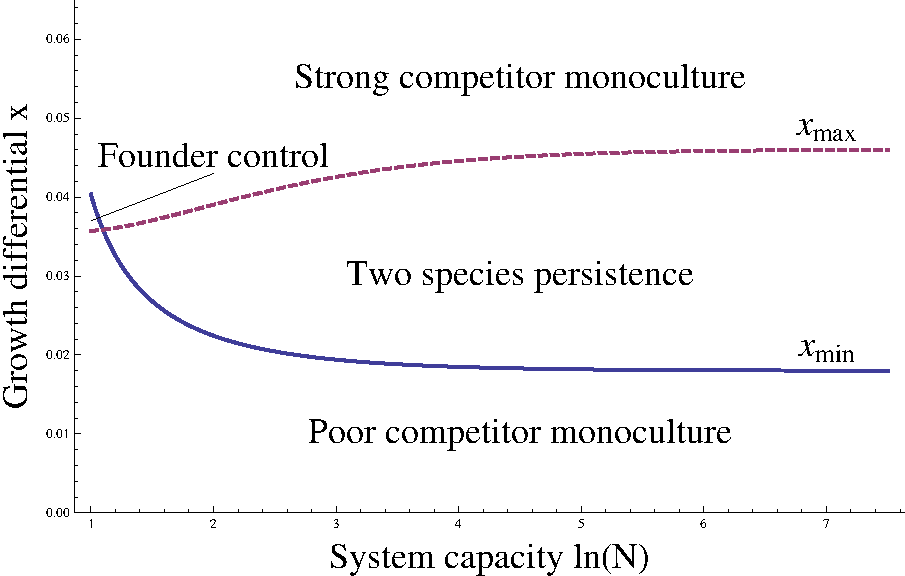
\includegraphics[width=4.5in]{xrangeofcoexist}
   \caption[Range of parameters giving coexistence without disturbance]{\textbf{Range of parameters giving coexistence without disturbance:} The effects of system capacity $N$ on the range of $x$ that will promote coexistence in the fecundity-growth trade-off model without disturbance. Should $x$ be too large, the more fecund species will likely be driven to extinction, while if the growth rates are very similar and $x$ drops below the lower limit then the more fecund species will competitively exclude the other species. When $x_{min}>x_{max}$ at low $N$, founder control occurs. Parameter values are $s_1=500,s_2=50$.}
 \label{fig:systemsize}
\end{figure}

When productivity is altered the effects depend on how productivity is implemented. Productivity, the production rate of new biomass, can be in the form of increased seed numbers (fecundity) or by increased juvenile growth rate. If juvenile growth rates are altered by a factor $\zeta$ for both species, then the effect is to alter the time $x$ for which species 2 can succeed with a secondary invasion by a factor $1/\zeta$, such that, for example, a doubling of juvenile growth rates halves the time species 1 juveniles spend vulnerable to competition.  In contrast, the effect of increased (or decreased) seed numbers by a factor $\phi$, with each individual therefore producing $\phi s_i$ seeds, is to increase (or decrease) the magnitude of the exponential term in $P(increase(n))$ and $P(decrease(n))$ by a factor $\phi$. This is equivalent to increasing (or decreasing) the time $x$ for which `invasion' is possible by the same factor. Note that if both growth rates and seed numbers vary with productivity the effective value of $x$ will be altered by a factor $\phi / \zeta$.

One further way that productivity can vary is if not all individuals are reproductively active at a given moment in time. Studies have demonstrated that the proportion of individuals producing seeds can vary widely, even over small spatial scales \citep{kettle2011seeing}. To model this, we assume that each individual produces seeds within a time step with probability $p$. We show in Appendix~\ref{app2c} that reducing productivity in this way results in a new coexistence range
\begin{equation}
\label{xrangep}
\frac{N\ln \left( \frac{p^2 s_1(N-1)(N-2)}{((N-1)p-1)(ps_1(N-2)+s_2)} \right)}{s_2}<x<\frac{\ln \left( \frac{(N-1)ps_1}{s_1+ps_2(N-2)}\right) N}{ps_2(N-2)}.
\end{equation}
which asymptotes to
\begin{equation}
\frac{1}{p}\left(\frac{1}{s_2}-\frac{1}{s_1}\right)<x<\frac{\ln\left(\frac{s_1}{s_2}\right)}{ps_2}
\end{equation}
as system capacity $N$ tends to infinity. This has two notable effects as system capacity increases. First, as when individual seed values are reduced ($\phi<1$), the values for $x_{min},x_{max}$ are increased (by a factor $1/p$). The result of this increase is that larger differences in growth rates between species can give coexistence, when compared to the coexistence range when $p=1$. Second, $x_{min}$ as given by \eqref{xrangep} has an asymptote at $N=1/p$, where the value of $x_{min}$ is infinite. Since coexistence requires $x>x_{min}$, coexistence cannot occur on average for systems with capacity smaller than the threshold $N=1/p$. Therefore, as $p$ decreases, and less individuals produce seeds at a given time, larger systems are required to get coexistence of both species as shown in Figure~\ref{fig:pnondist}.  
\begin{figure}[th]
\centering
   \begin{tabular}{rrrr}
   (a)&&(b)&\\
  &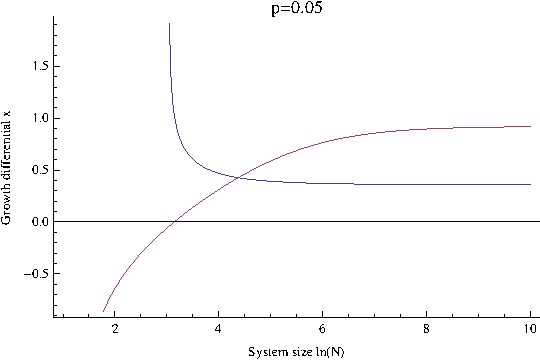
\includegraphics[width=2.5in]{p005nondist.pdf} && 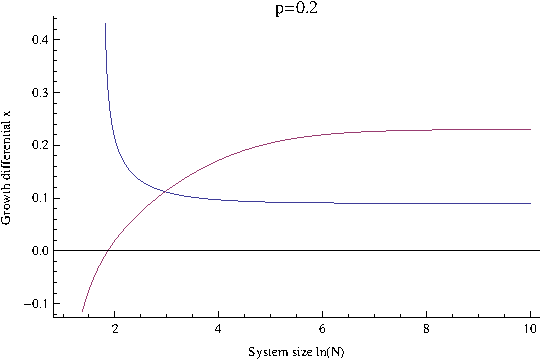
\includegraphics[width=2.5in]{p020nondist.pdf} \\
  (c)&&(d)&\\
  &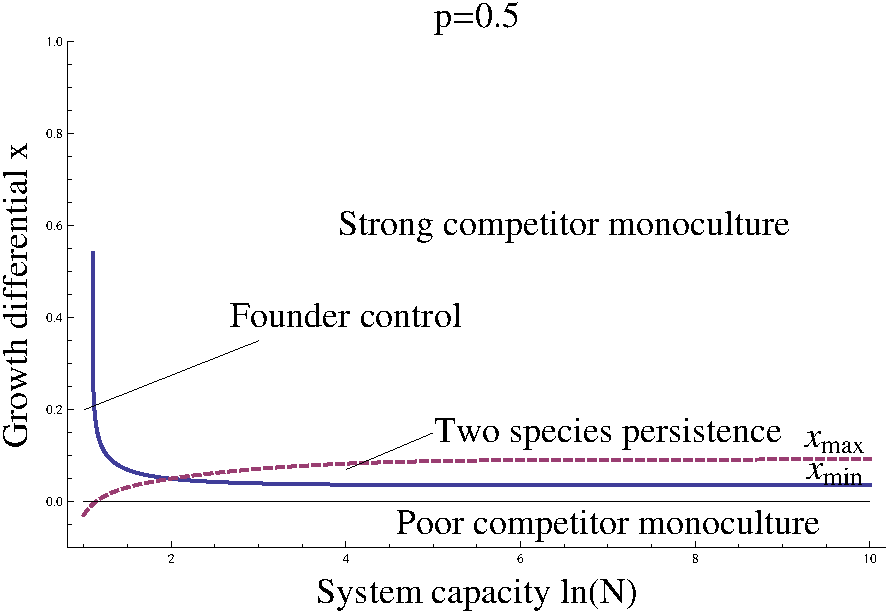
\includegraphics[width=2.5in]{p050nondist.pdf} && 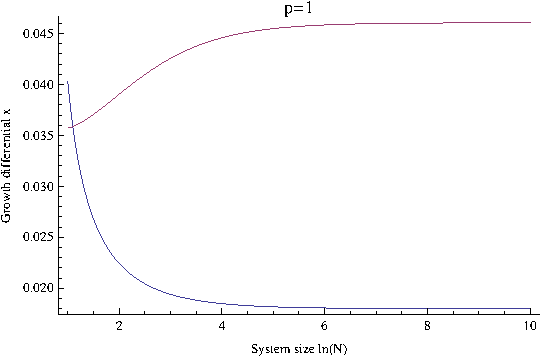
\includegraphics[width=2.5in]{p100nondist.pdf} \end{tabular}
   \caption[Coexistence without disturbance for reduced productivity]{\textbf{Coexistence without disturbance for reduced productivity:} The effects of altering the probability $p$ of an individual being reproductively active on the range of growth differential $x$ that gives coexistence, and how this varies with $N$, in an environment with no disturbance. Decreasing $p$ results in larger values of $x$ predicting coexistence, while simultaneously requiring larger system capacity $N$ to give this region of coexistence. Parameter values $s_1=500, s_2=50$.}
 \label{fig:pnondist}
\end{figure}


\subsection{The effects of disturbance events} \label{ss:resultsdist}
When disturbance events are introduced, there are three possible scenarios to study. First, when $x<x_{min}$, so that in the absence of disturbance the more fecund species 1 will exclude species 2, disturbance events cannot increase diversity by supporting the second species. Second, if the system can exhibit coexistence in the temporally homogeneous environment, moderate levels of disturbance (disturbance events with low intensity $I$ or very low frequency $f$) will retain this coexistence, with a shift in equilibrium abundances towards greater numbers of the more fecund species (results not shown). However, large intensities with intermediate or high frequencies will lead to a loss of diversity, creating a monotonically decreasing DDR, as species 1 will competitively exclude the less fecund species 2. The third scenario is more interesting: when $x>x_{max}$, where in the absence of disturbance, the stronger competitor will competitively exclude the more fecund species. Then it is possible that disturbance can promote coexistence. If the IDH holds, we would expect to see the species richness to increase then decrease as the size of disturbances is increased. Substituting the functions \eqref{increase}, \eqref{decrease} and \eqref{sp1} into the function given by \eqref{avchange} we can plot the region of $f-I$ parameter space that satisfies \eqref{ac1} and \eqref{acn-1}, revealing a region where long term coexistence occurs (Figure~\ref{hockey}).  The boundary of this region is where approximately half the simulations are expected to exhibit coexistence. In Appendix~\ref{app2d} we examine how time series simulations match the predictions given by using the approximation given by \eqref{avchange}, and note that for high intensity disturbances, the approximation becomes less accurate (see also Appendix~\ref{app2a}). When intensity $I=1$, at the first disturbance event, all individuals die, and so neither species survives in the environment, and coexistence does not occur. However, in evaluating the expected change, the function is weighted towards non disturbance events when frequency $f$ is low. This can lead to an underestimation of the effects of high intensity disturbance events, and predict coexistence for parameters where the death of both species is inevitable.
 Outside of this region with very high intensity, the approximation accurately captures the behaviour of simulations.

\begin{figure}[th]
\centering
  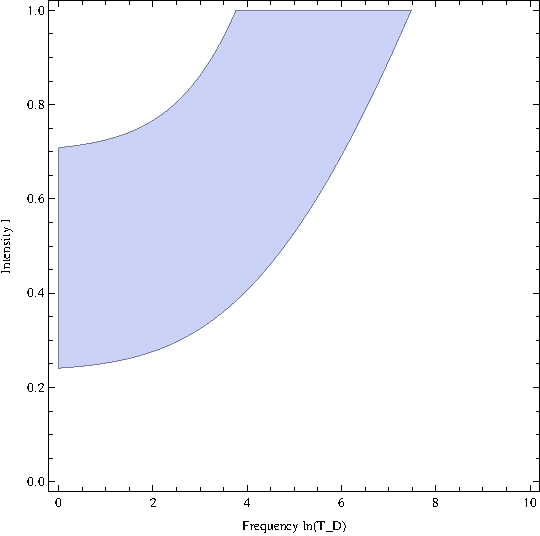
\includegraphics[width=5in]{hockeyTd.pdf}
   \caption[Coexistence with disturbance]{\textbf{Coexistence with disturbance: }The region of coexistence (shaded area) for $x>x_{max}$ when $p=1$, and all individuals produce seeds within every event time step. Changes in disturbance frequency or intensity can produce different DDRs, with the humped, unimodal DDR predicted by the IDH one of several possible outcomes. Parameter values (a) $s_1=500, s_2=50, x=0.06,N=1000$.}
 \label{hockey}
\end{figure}

Analysis shows that it is possible to get very differently shaped DDR curves in this model, and this is affected by which factor influencing disturbance is considered. Increasing intensity can give very different responses to altering the frequency of disturbances. If $f=(dNT_D)^{-1}$ is fixed such that $1/f<T$, where $T$ is the expected time to extinction (see Appendix~\ref{app2b}), increasing intensity will give a humped DDR. For example, if $\ln(T_D)=1$ is fixed in Figure~\ref{hockey}, and intensity increased from $I=0.1$, we initially see an increase in diversity as intensity crosses the point $I\approx0.25$. As intensity is increased further, however, there is a decline in diversity at $I\approx0.72$. This produces the classic peaked DDR predicted by the IDH.

However, if the fixed frequency is low, coexistence is impossible for any intensity $I$, and so a flat DDR is produced. Meanwhile, if intensity $I$ is fixed, while frequency of disturbance is varied, there are three possible scenarios: i) When $I$ is low (e.g. $I=0.1$), the stronger competitor, species 2, will dominate regardless of frequency; ii) For intermediate intensities (e.g. $I=0.5$), increasing frequency will cause diversity to increase from one species to two (when $\ln(T_D)\approx 5$ for $I=0.5$), a monotonically increasing DDR; iii) When intensity is high (e.g $I=0.8$), increasing frequency will match the predictions of the IDH, giving a peaked DDR with coexistence occurring for intermediate frequencies (when $I=0.8$, the peak in diversity is predicted in the range $2\leq \ln(T_D) \leq 6$). However, this coexistence occurs for a narrow range of $f$ (Figure~\ref{fig:simulationdata} in Appendix~\ref{app2d}). 

Increasing system capacity has a similar effect as in the non disturbance case, where increasing systems size can increase the range of parameters that give coexistence slightly, but the region of coexistence asymptotes quickly to a fixed region of parameter space as $N$ increases. This is caused by a stabilisation of the relationship between the dominant eigenvalue that determines the speed of community dynamics, and the number of events that occur in a fixed time period. With a fixed death rate (here 1\% per year), the number of events that occur per year in the present model scales linearly with system capacity, such that in a forest twice as large, we can expect to observe twice as many death events each year. As shown in Appendix~\ref{app2b}, the eigenvalue that determines the pace of the dynamics, and thus the time to converge to either the boundary or the internal quasi-equilibrium, asymptotes in a non linear fashion to $1$. For small systems ($N<300$), an increase in system size will have an exponential effect on increasing the time to extinction. This extended time to extinction increases the likelihood of an infrequent disturbance event occurring before extinction. In other words, a long transient towards a community dominated by a competitively dominant (e.g. shade-tolerant, late-successional) species will enable a shade-intolerant, pioneer species to be maintained before the next disturbance event shifts the environment into its favour. Once $N$ increases above a certain value, the change in time to extinction as a function of system capacity can be approximated by a linear relationship. Thus, owing to this linear relationship, while the time to extinction (measured in events) doubles as system capacity is doubled, the same change occurs in how many events are expected to occur. Therefore, the disturbance frequencies that give coexistence (for a given intensity) remain unchanged as system capacity increases further. This ensures that the systems response to disturbance regimes is robust to changes in system capacity.

These results are also robust to changes in productivity. A decrease in growth rates or increase in average seed production (such that $\phi/\zeta>1$) will shift the values of $x$ that give coexistence without disturbance to lower values. This in turn causes a shift in the disturbance intensities $I$ that give coexistence for a fixed $x$. If $x \in (x_{min},x_{max})$, this change in productivity can cause the value of $x_{max}$ to move below $x$, which means that low intensity disturbances may no longer  give coexistence. If species 2 excludes specie 1 in the absence of disturbance, increasing $\phi/ \zeta$ will move the diversity peak where both species coexist to higher disturbance intensities, matching the predictions of dynamic equilibrium models (Huston 1979; Kondoh 2001). In contrast, reducing $\phi/\zeta$ by increasing growth rates or decreasing seed production will increase the values of $x$ for which coexistence occurs without disturbance (as determined by \eqref{xrangep}).This has the effect of lowering the intensities for which coexistence can occur.

However, while a change in productivity can alter the range of disturbance regimes for which coexistence occurs for a given set of parameters, the qualitative results do not change. Using an approximation for the expected change when individuals are reproductive with probability $p<1$(outlined in Appendix~\ref{app2e}) it is possible to see that when seed production in decreased, the results are qualitatively similar, displaying a `hockey stick' type shape to the coexistence region (Figure~\ref{pfigure}). Figure~\ref{pfigure} also shows how reducing $p$ has similar effects to a reduction in the value of $x$. While the asymptote to a fixed region as $N$ increases is slightly slower when $p$ is reduced, coexistence still asymptotes to a fixed region as we increase system capacity, demonstrating that these results are robust to changes in both productivity and system capacity.

\begin{figure}[htbp]
\begin{center}
\begin{tabular}{cccc}
(a)&&(b)&\\
&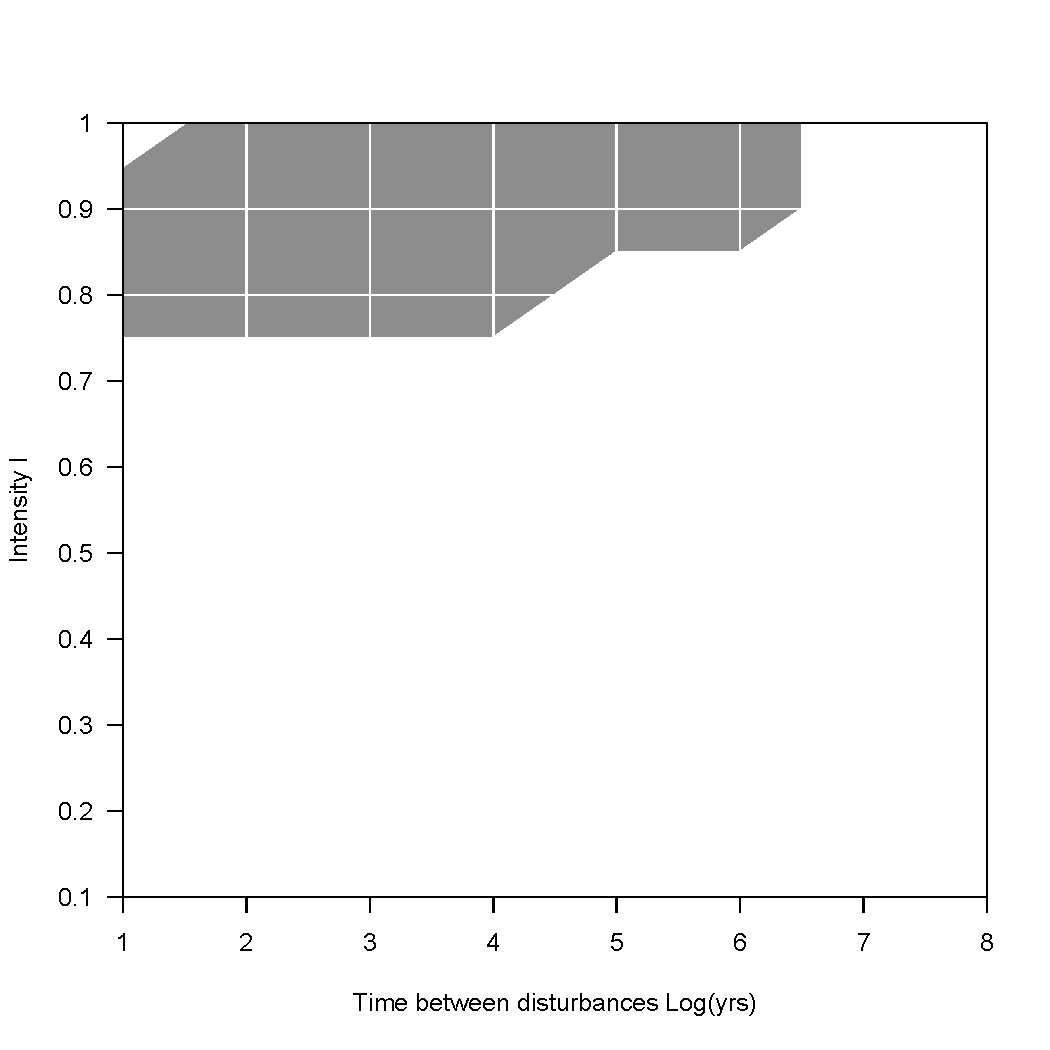
\includegraphics[width=2.5in]{pplot75.pdf} &&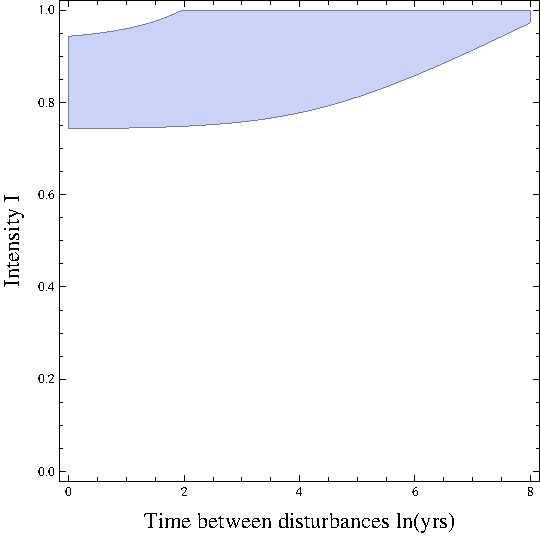
\includegraphics[width=2.5in]{p0p75xequiv.pdf}\\
(c)&&(d)&\\
&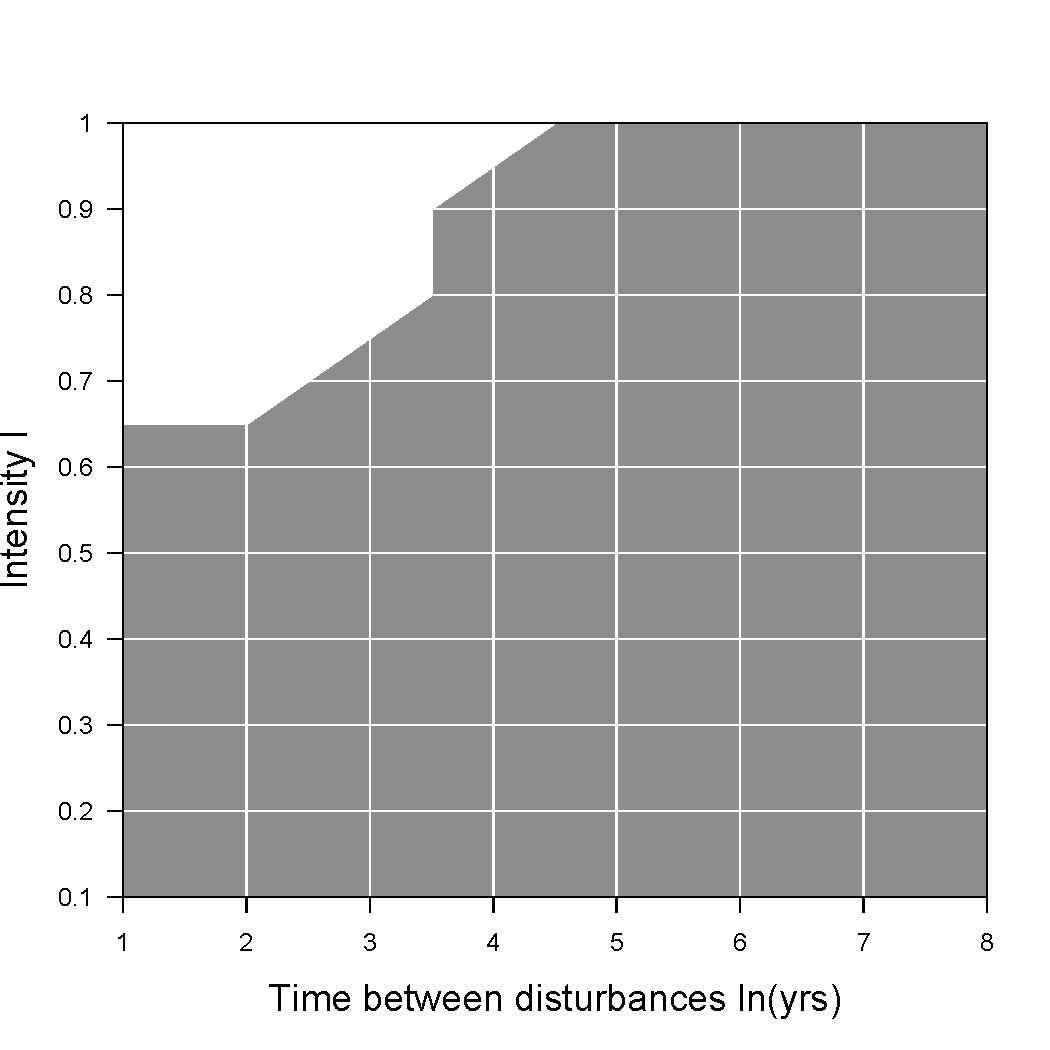
\includegraphics[width=2.5in]{pplot10.pdf} &&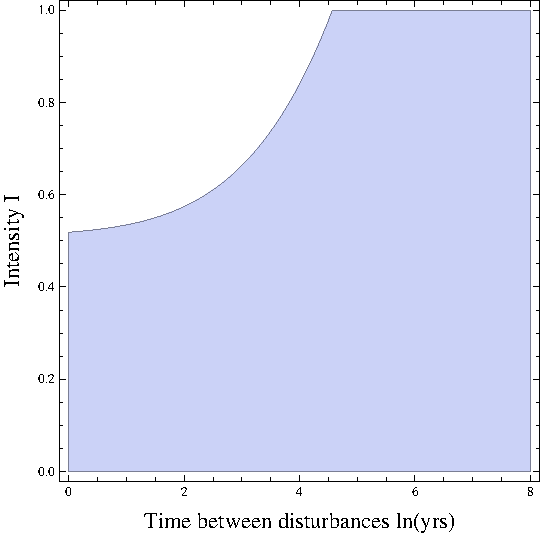
\includegraphics[width=2.5in]{p0p2xequiv.pdf} \end{tabular}
\caption[Coexistence with disturbance for reduced productivity]{\textbf{Coexistence with disturbance for reduced productivity:} The effect of reducing the probability of an individual being reproductively active $p$ on the disturbance regimes that predict coexistence. Reducing $p$ has a similar effect as transforming the growth rate differential $x \to px$. Shaded areas are where coexistence is predicted. (a) and (c) show the region of predicted coexistence using the approximation given in Appendix~\ref{app2e} for $s_1=500,s_2=10,x=2$ for (a) $p=0.75$ and (c) $p=0.1$. The approximation is evaluated at $\ln(T_D)=i, I=0.1j$ for alll $i\leq8, j\leq 10$, and a linear extrapolation used between points (b) and (d) illustrate that the effect is the same as reducing $x$ to (b) $x=1.5$ and (d) $x=0.2$. Note that $x_{max}=\ln(500/10)/10\approx 0.39$, such that (c) and (d) represent parameters where coexistence occurs in the absence of disturbance.}
\label{pfigure}
\end{center}
\end{figure}


\section{Discussion} \label{discuss}
Disturbance is often considered an important driver of biodiversity and species richness \citep[e.g.][]{denslow1987tropical,lawton1988natural,sousa1984role}. We use a lottery type model to confirm that while it is possible for two species to coexist along a fecundity-growth trade-off in a homogeneous environment, disturbance events can dramatically increase the range of parameters for which coexistence is possible. Analysis shows, in accordance with recent theory \citep{miller2011frequency}, that different factors influencing disturbance (here frequency or intensity) can have very different effects, and may impact species richness in different ways. We add to this theory by determining analytic conditions for coexistence under given disturbance regimes, and by demonstrating that these conditions are robust to model type, productivity and system size. We suggest these general results may explain in part some of the conflicting empirical results regarding the IDH. Indeed, one consequence of our results is that it is possible for two forest fragments to exhibit different diversity patterns, even though all species in both sites have the same vital rates (i.e. same seed productivity and growth rates). Further, an increase in either disturbance frequency or intensity can have different effects, and these effects are dependent on the underlying disturbance regime. For example, a region with infrequent disturbances of intermediate intensity may show an increase in diversity as disturbances become more frequent, while a different forest with more frequent yet less intense disturbances may not exhibit this increase in diversity with frequency (see Figure~\ref{hockey}).

In general, our results indicate that it is important to consider the intensity and frequency of disturbance events as separate parameters when studying the effects of disturbance on diversity levels, and emphasise that past disturbances can have long-lasting effects, which persist for decades or centuries, in accordance with \cite{foster1999human}. In the current model, these effects come in the form of persistence of inferior competitor species, which can be sustained for many time steps between disturbances as infrequently as every 400 years. The result here is increased diversity within the canopy, but disturbance can effect several other aspects of the environment, such as net primary production \citep[e.g.][]{turner2010disturbance}. These results, while arising in a new model, are qualitatively similar to those of \cite{miller2011frequency}, adding weight to the suggestion that the separation of factors controlling disturbance is an important consideration in studying the effects of disturbance on a community. We build on this work by showing that these qualitative results are extremely robust to changes in system capacity and productivity.

Our results also demonstrate that frequency and intensity can have different effects across a broad range of system capacities and productivity levels. The model reproduces the results of \cite{kondoh2001unifying} when disturbance frequencies are high, showing a diversity peak at lower disturbance intensities  when productivity is reduced. We also find that disturbance regimes that maximise coexistence may be predicted by a combination of system productivity and the life histories of species in the community. However, these results are not applicable to alternative measures of disturbance. For example, a moderate change in productivity has negligible effect on the community response to increased frequency. We therefore demonstrate that the results of Kondoh are not universal, further emphasising the importance of considering different factors determining disturbance.

Many plant populations are thought to be recruit limited \citep[e.g.][]{clark1998stages,eriksson1992seed,svenning2005seed}, and this may be particularly important in very species rich communities, where most species are locally quite rare \citep[e.g.][]{svenning2005seed}. By relaxing the assumption that all individuals are reproductively active at the time of the disturbance, or otherwise altering the seed production in the system, we also show the importance of seed limitation on the community dynamics. Our analyses show that seed limitation generally increases difference in growth rates that allow species to coexist, and this is in line with previous theory that shows recruit limitation often slows dynamics, especially in species rich communities \citep{hurtt1995consequences}. This again suggests that processes that slow down the dynamics will act to help support the maintenance of competitively weaker (e.g. pioneer) species. While modelling sexual (non-selfing) species would require a different analysis, sexual species may experience slower dynamics because they become both pollen and seed limited with pollen limitation leading to reproductively active trees not bearing fruit. The consequences of sexuality in this context remain an open question, and a more detailed model approach may be necessary.

Another aspect in which our results differ from those of  \cite{miller2011frequency} is that at very high frequencies, their model exhibited a tailing off of coexistence \citep[Figure 1 of ][]{miller2011frequency}, resulting in a crescent shaped region of coexistence. Our model does not  present this tailing off, and even when $f=1$, a relatively broad range of intensities can give coexistence. We suggest that this is because our model allows for full site replenishment following a disturbance event before a second disturbance is possible. Our assumption makes the model computationally much simpler, at the expense of some realism. However, the assumption of full replenishment will only alter outcomes at very high intensities, where very few individuals survive. In the case where at least 2\% of the system survives a disturbance event, this would allow for complete replenishment, on average, between very common disturbance events, such as El Nino, which strikes with a frequency of approximately once every 5 years. When the system considered is shrub- or grassland, we anticipate that site replenishment will also be rapid.

While we only consider two species in the current model, previous work has argued that disturbances may enhance coexistence i multi-species communities \citep[e.g.][]{loehle2000strategy,roxburgh2004intermediate}. Earlier theory has suggested that infinitely many species can coexist along a spatially implicit competition-colonisation trade-off \citep[e.g.][]{tilman1994competition}, and that spatial structure is not necessary for generating large numbers of species \citep{adler2000space} although for large numbers of species coexistence is highly unlikely \citep[Chapter~1;][]{nattrass2012quantifying}. Further, \cite{gyllenberg2005impossibility} show that the coexistence of infinitely many species is structurally unstable. Chapter 4 of this thesis considers models featuring greater species numbers, which we anticipate will produce qualitatively similar results, with many different diversity curve shapes generated by different combinations of frequency and intensity, even when the overall biomass loss due to disturbance is identical. The key element to generating coexistence is that no one species is superior across the entire range of disturbance gradient, and this means further underlying niche differences are required in order to support higher number of species \citep[e.g.][]{seifan2013beyond}. Nonetheless, comparisons of different forests with different levels of disturbance frequency and intensity do exist. For example, \cite{denslow1987tropical} reports on two forests, one in Puerto Rico which has not experienced any hurricanes in the last 150 years, and one in Costa Rica which experiences a hurricane once every 20-30 years. Despite having otherwise similar annual rainfall and topology, the former site supports only 88 tree species in 16ha of study plots, whereas the latter supports 269 species in 12.4ha of plots. Although other differences are apparent, such as the amount of human activity and isolation from the mainland, the Costa Rican forest does have a faster turnover of trees caused by tree fall and the theory presented here does predict forest with the more frequent but less intense disturbances to have the fewer species.

The current model does not include spatial heterogeneity. Previous studies suggest that spatial structure does not have a significant effect of disturbance events and their aftermath in a number of circumstances, such as when the disturbance does not have directionality \citep{frelich1991natural}. However, given that most seeds of most plants fall near to the parent, incorporating realistic dispersal kernels could influence the relative importance of disturbance to the community dynamics. Many plant communities show within-species clustering, meaning nearby neighbours are quite likely to be conspecifics \citep{condit2000spatial,murrell2001uniting}, and deaths of individuals leave gaps that most likely to be exploited by these neighbours. Generally speaking it is expected that such localised dispersal should slow down the community dynamics both in terms of time to expected exclusion (Gandhi et al. 1998) and also potentially during the invasion process \citep{murrell2010does}. Which of these two effects dominates remains an open question for the model presented here, and metapopulation theory suggests the effect on the dynamics might be quite complex \citep{ovaskainen2002transient}. However, we suspect in many cases the effect of restricted dispersal on all species will help maintain the weaker competitor in the community because restricted dispersal will mean it can win some sites uncontested.

Often, disturbance is modelled using a single parameter, as reviewed by \cite{shea2004moving}, yet we demonstrate that identical overall disturbance rates can produce different environmental conditions, and different diversity levels. This extends to the consideration of diversity curves as disturbance is varied. The same change in overall disturbance levels can result in dramatically different diversity curves, with monotonic curves and both peaked and U-shaped curves, although the latter are difficult to achieve. These results are in accordance with the findings of \cite{mackey2001diversity}, who report that peaked and monotonic DDRs are all relatively frequent, while U-shaped curves are much rarer. The differences in effect on biodiversity between the factors governing the total level of disturbance could therefore suggest an explanation for the great variety of DDR shapes observed in nature. While we only consider two of these factors, frequency and intensity, we find that an increase in intensity will often give a humped DDR, while an increase in frequency of disturbance will present a monotonic or flat DDR, and this is robust to changes in all model parameters. Once other factors of disturbance are considered, a still broader range of DDR shapes may be explained by the variation of how disturbance is measured. Some recent empirical work has considered the effects of different disturbance measures \citep[e.g.][]{bertocci2005contrasting,collins1987interaction,svensson2009equal}, and the work presented here suggests that it should remain a point of emphasis for empirical studies.


\section*{Appendices}

\bappendix
\section{Approximating the expected change function}
\label{app2a}
 When approximating the average change using the function given by \eqref{avchange}, we must compare these results to the actual expected change. Using the Law of Total Probability ($P(A)=\sum_{b \in B} P(A|b)P(b)$), where $A$ is the probability of increasing species 1 numbers by $k$ individuals, and $B$ the set of possible death numbers in species 2, and summing the results weighted by $k$, the average change at the boundaries is given by
\begin{align}
\label{acreal1}&AvCh(1)=\frac{-I+(N-1)I^{N-1}(1-I)}{dNT_D}\\
&+\frac{(1-I)\sum_{k=1}^{N-2}\sum_{j=k}^{N-2}k I^j(1-I)^{N-2-j}{N-2\choose j} Sp_1(1,N-1-j)^k(1-Sp_1(1,N-1-j))^{j-k} {j \choose k}}{dNT_D} \notag \\
 &+ \left(1-\frac{1}{dNT_D}\right)(P(\text{Increase}(1))-P(\text{Decrease}(1))), \notag \\
 \label{acrealtot}&AvCh(N-1)= \frac{-I^{N-1}(N-1) +I(1-I^{N-1})}{dNT_D} \\
 &-\frac{(1-I)\sum_{k=1}^{N-2}\sum_{j=k}^{N-2}k I^j(1-I)^{N-2-j}{N-2\choose j} Sp_1(1,N-1-j)^{j-k}(1-Sp_1(1,N-1-j))^{k} {j \choose k}}{dNT_D} \notag \\
 &+ \left(1-\frac{1}{dNT_D}\right)(P(\text{Increase}(N-1))-P(\text{Decrease}(N-1))). \notag
  \end{align}
where $Sp_1$ is as defined in \eqref{sp1}. Since these sums become computationally expensive for large system size, we approximate these using \eqref{avchange}. Figure~\ref{fig:approxerror1} shows how the error varies when \eqref{avchange} is used to approximate \eqref{acreal1}. The error of the approximations decreases with increased time between disturbances $T_D$, decreased intensity $I$, and increased system capacity, while Figure~\ref{fig:approxerrortot} shows the same effects of system size and disturbance frequency for approximating the average change when $N-1$ sites are occupied by species 1 given by \eqref{acrealtot}. However, in this case the relationship between error and intensity exhibits a peak in error size for intermediate intensities. This may be because for the upper boundary condition \eqref{acrealtot}, the exponential term in \eqref{sp1} exhibits greater variation than in \eqref{acreal1}, and that this error is maximised at intermediate values of $I$. While only the errors generated by one set of parameters are shown in Figures~\ref{fig:approxerror1} and \ref{fig:approxerrortot}, the qualitative results are robust to parameter changes.
 \begin{figure}[th]
\centering
   \begin{tabular}{rrrr}
   (a)&&(b)&\\
  &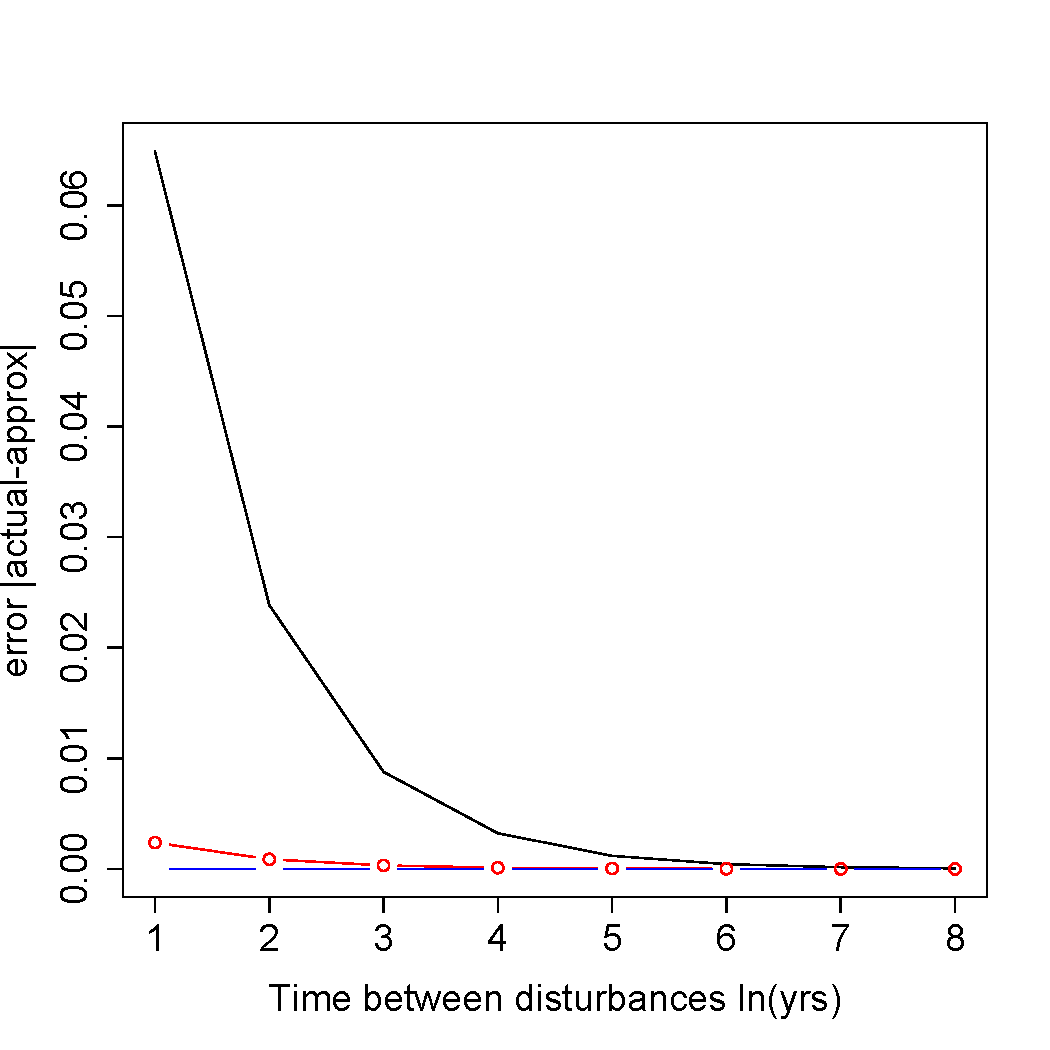
\includegraphics[width=2.5in]{errwithTlb.pdf} && 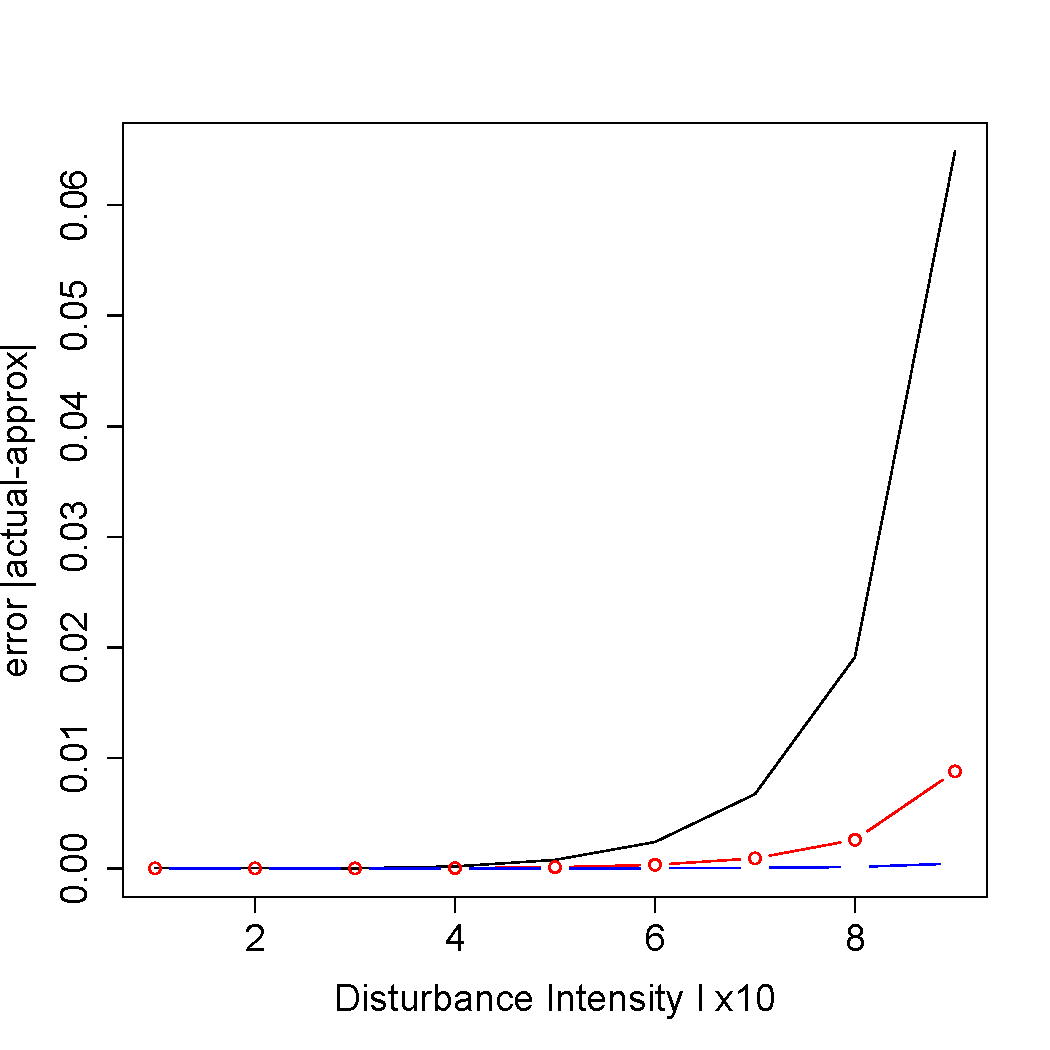
\includegraphics[width=2.5in]{errwithIlb.pdf} \\
  (c)&&(d)&\\
  &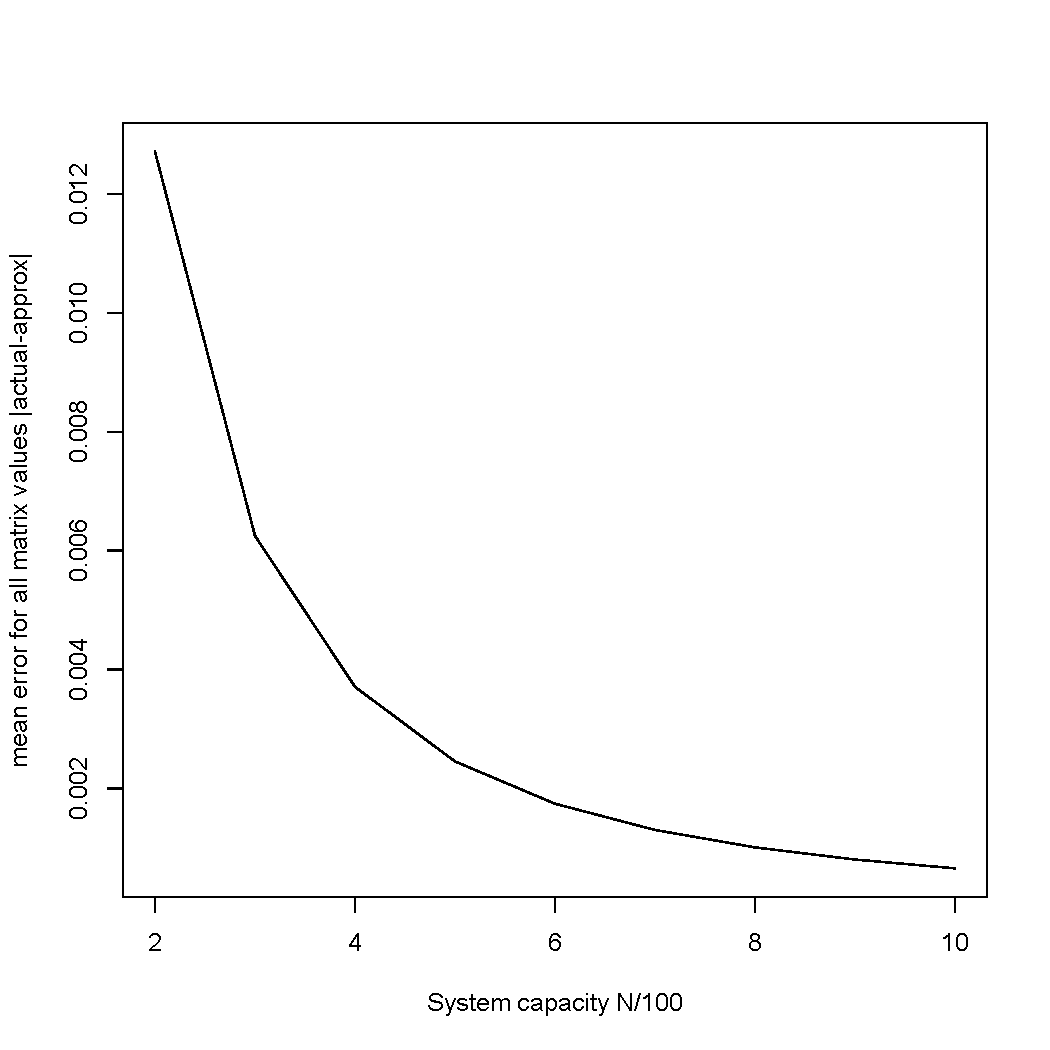
\includegraphics[width=2.5in]{meanerrorovermatrix.pdf} && 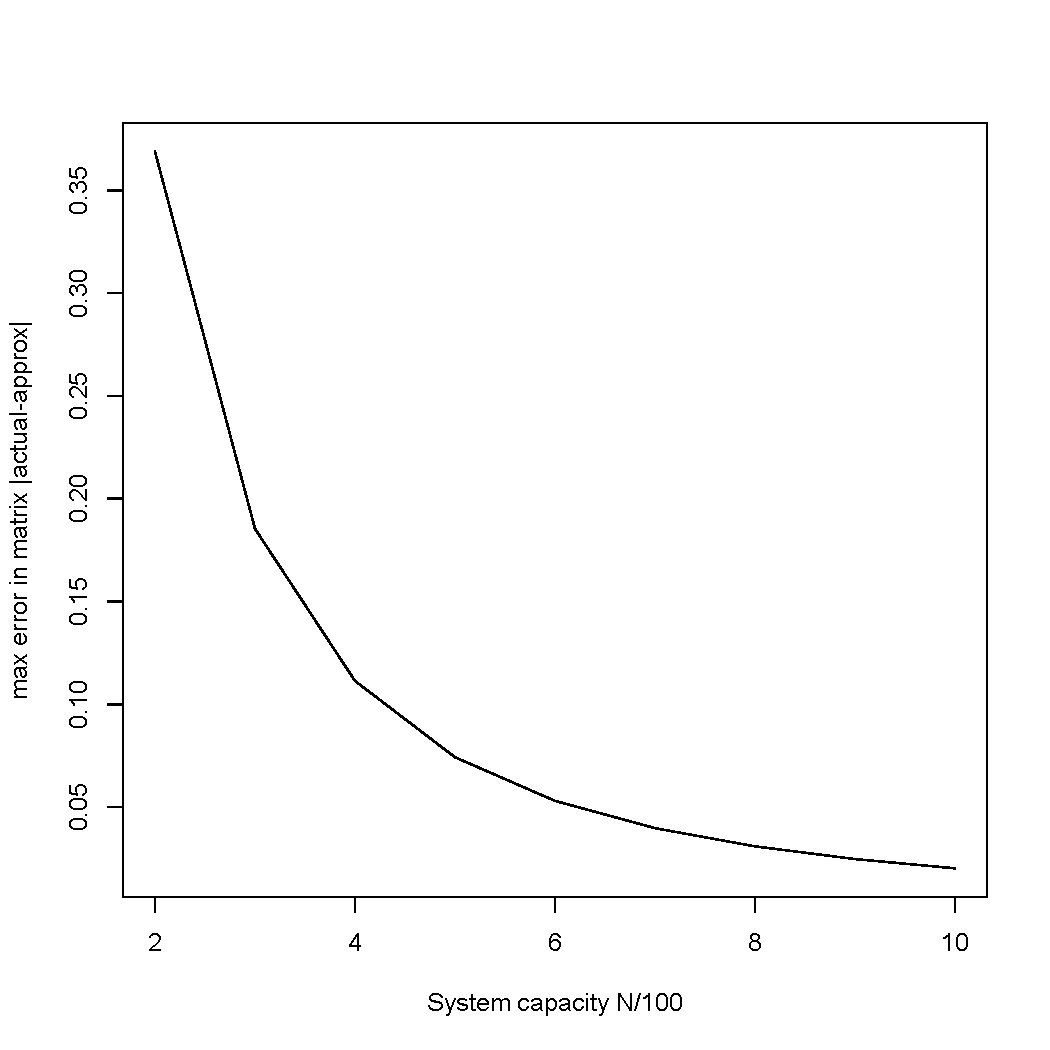
\includegraphics[width=2.5in]{maxerrorovermatrix.pdf} \end{tabular}
   \caption[Approximation errors for species 1 invasion]{\textbf{Approximation errors for species 1 invasion:} (a) How the error of the approximating function for species 1 invasion changes with increased time between disturbances $T_D$ for various intensities $I=0.3$ (blue, dashed lines), $I=0.6$ (red, dashed lines with points), and $I=0.9$ (black, solid line) (b) the effects of increasing intensity $I$ for fixed frequency $\ln(T_D)=1$ (black, solid line), $\ln(T_D)=4$ (red, dashed line with points) and $\ln(T_D)=8$ (blue, dashed line).. Errors are larger for higher intensity, but decrease as the expected time between disturbances increases. (c-d) How the mean (c) and maximum (d) error size decrease with increased system capacity $N$. The error was calculated for intensities $I=0.1,0.2,0.3,...,0.9$ and time between disturbances $\ln(T_D)=1,2,3,...,8.$ Parameters used are $s_1=500,s_2=50,x=0.06,N=500$.}
 \label{fig:approxerror1}
\end{figure}
 \begin{figure}[th]
\centering
   \begin{tabular}{rrrr}
   (a)&&(b)&\\
  &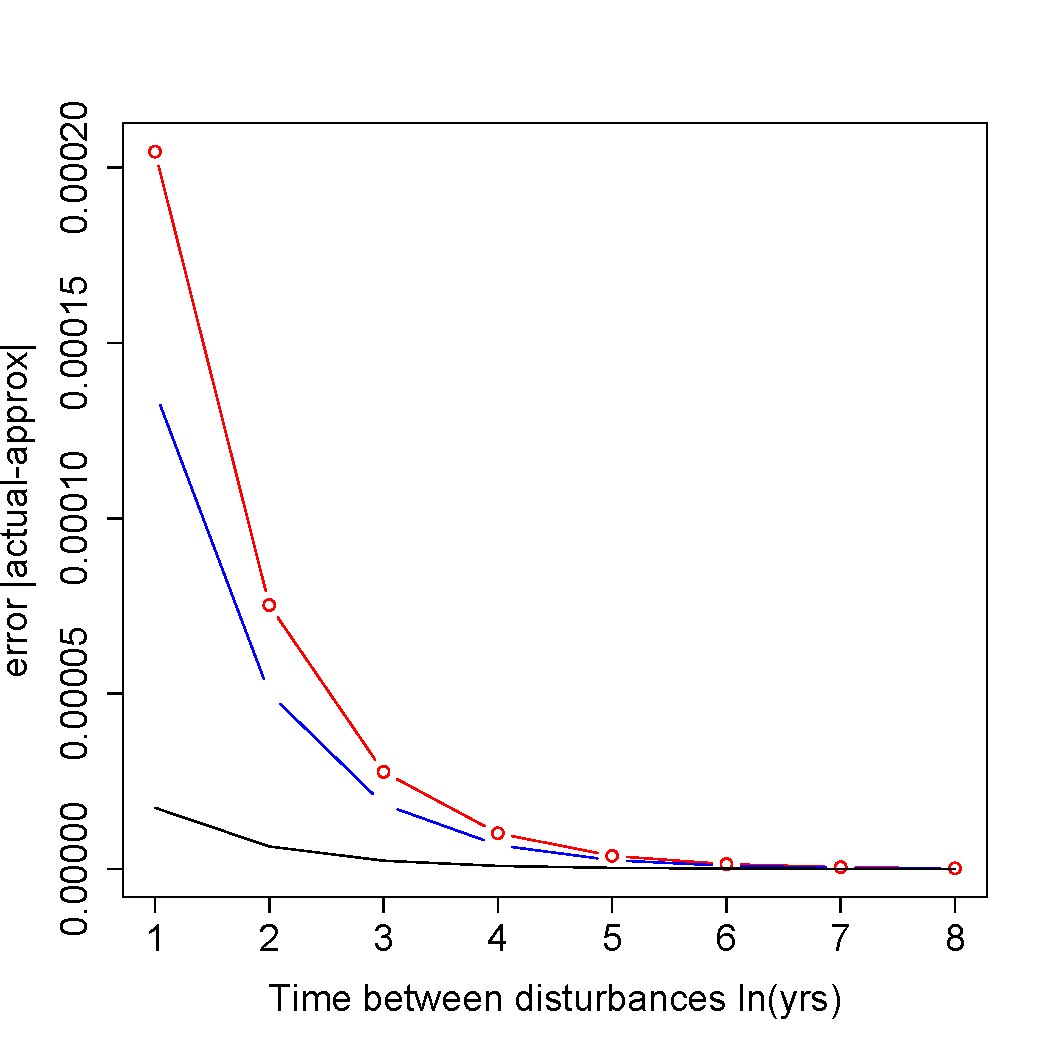
\includegraphics[width=2.5in]{errwithTub.pdf} && 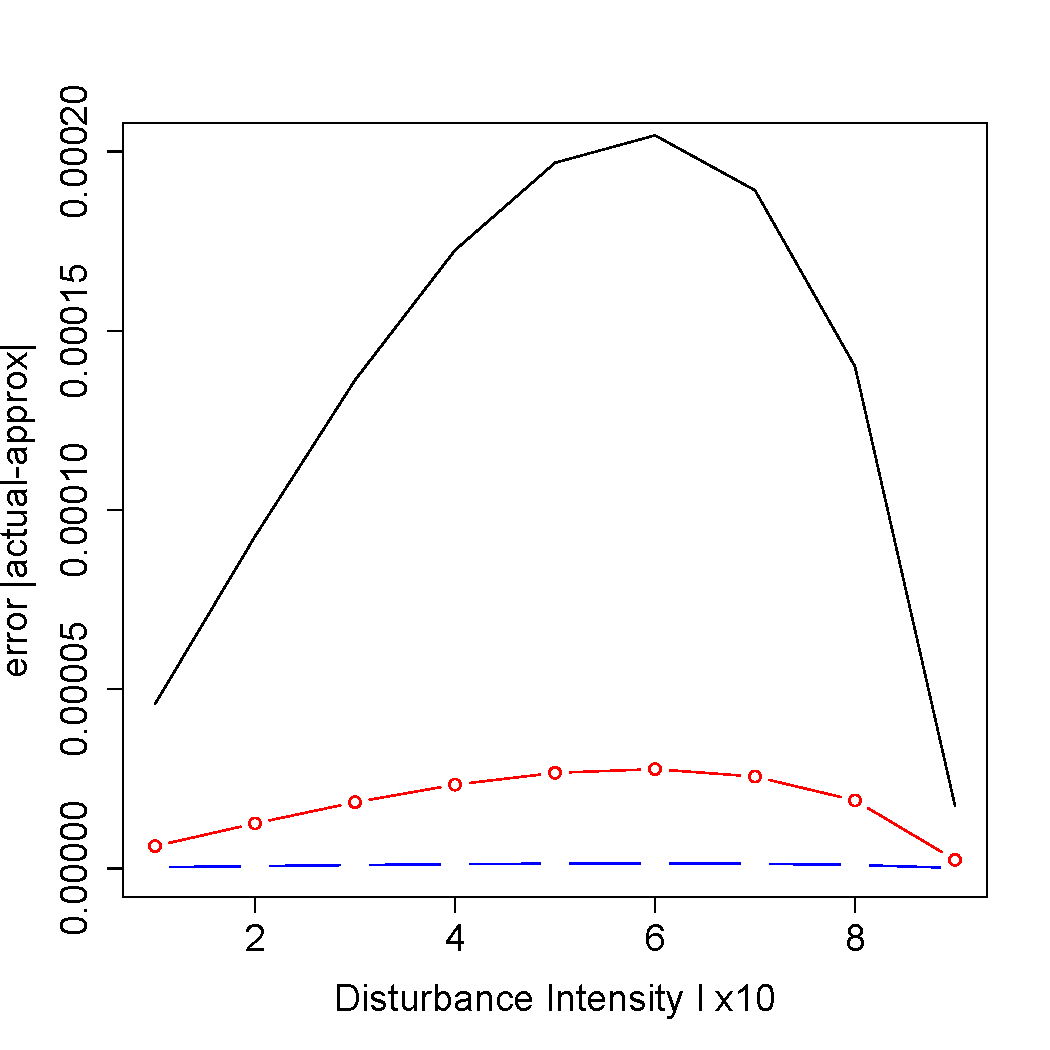
\includegraphics[width=2.5in]{errwithIub.pdf} \\
  (c)&&(d)&\\
  &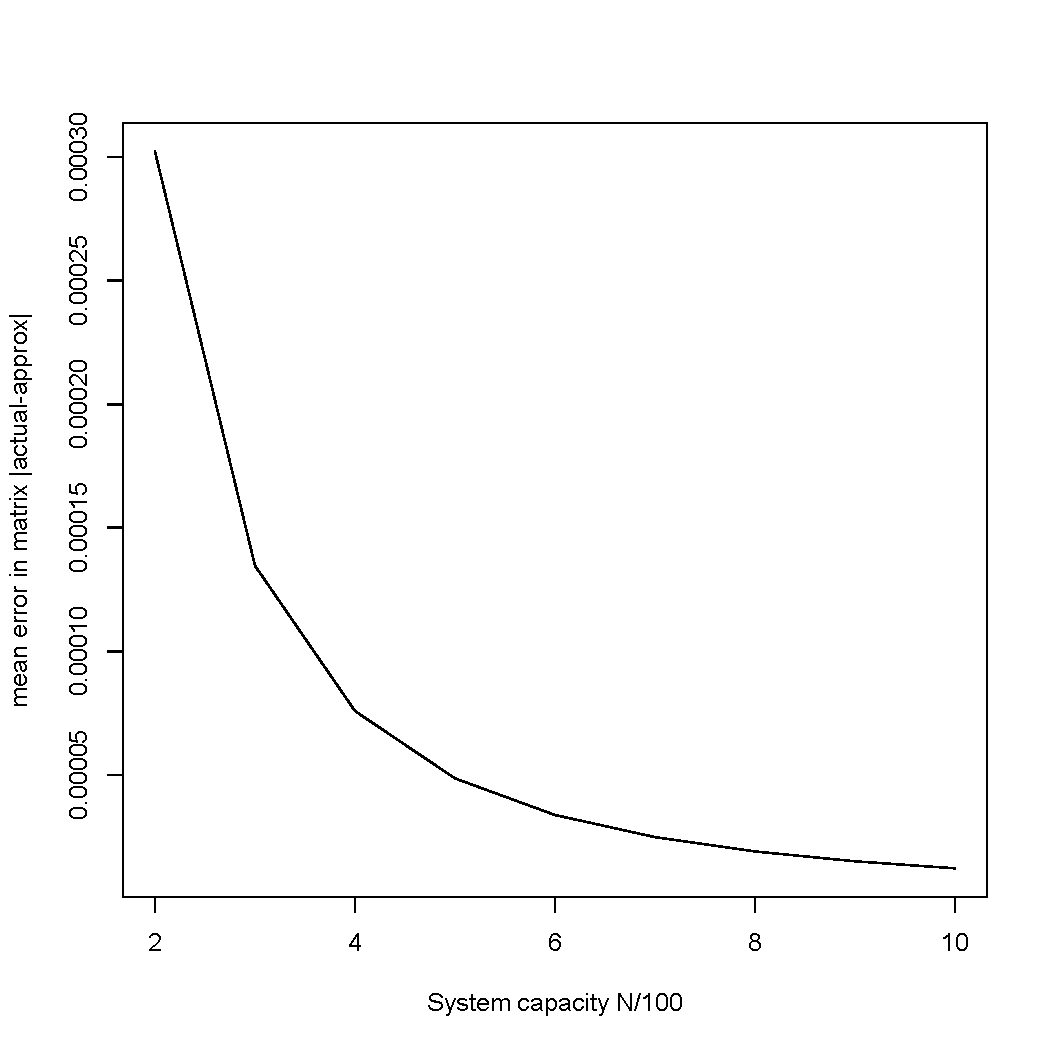
\includegraphics[width=2.5in]{meanerrortotovermatrix.pdf} && 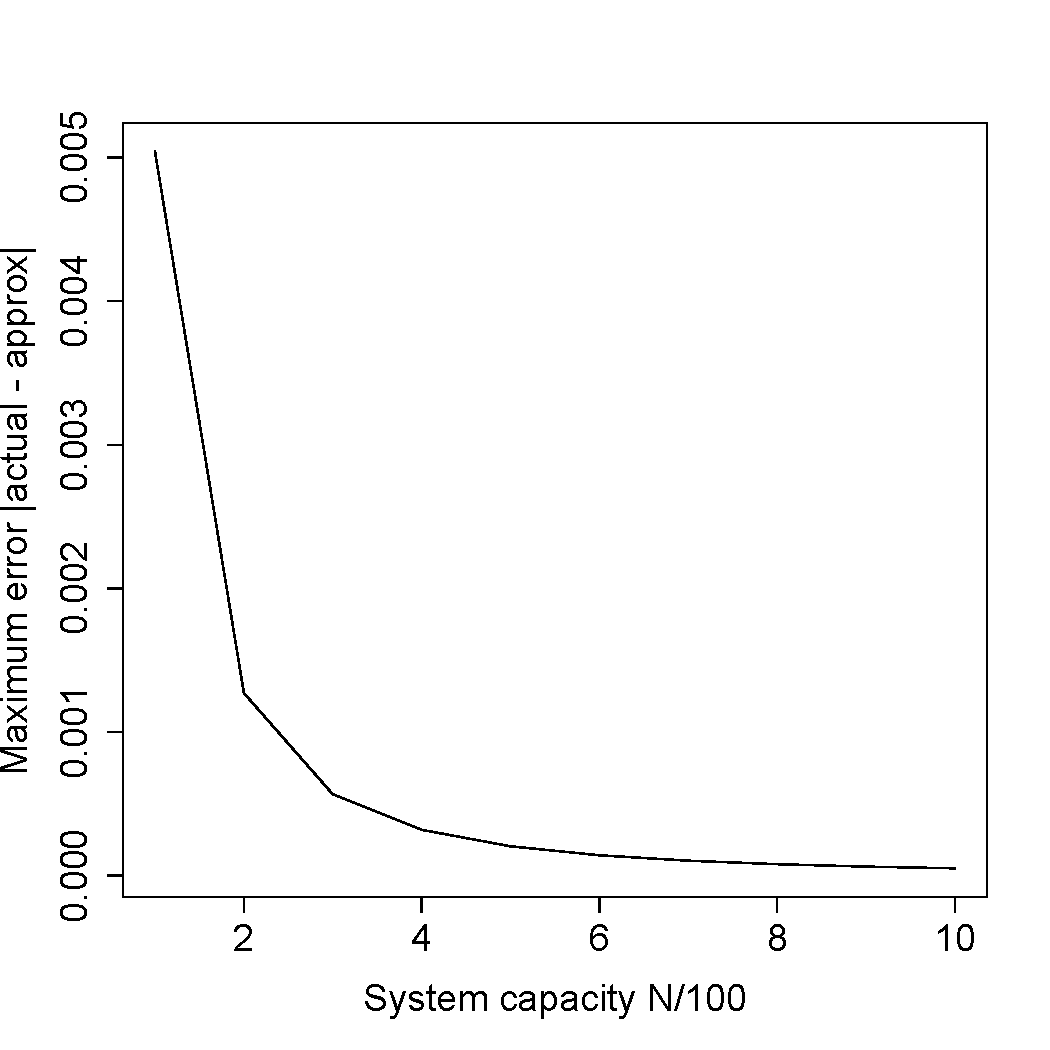
\includegraphics[width=2.5in]{maxerrortotovermatrix.pdf} \end{tabular}
   \caption[Approximation errors for species 2 invasion]{\textbf{Approximation errors for species 2 invasion: }(a) How the error of the approximating function for species 1 invasion changes with increased time between disturbances $T_D$ for various intensities $I=0.3$ (blue, dashed lines), $I=0.6$ (red, dashed lines with points), and $I=0.9$ (black, solid line) , and (b) the effects of increasing intensity $I$ for fixed frequency $\ln(T_D)=1$ (black, solid line), $\ln(T_D)=4$ (red, dashed line with points) and $\ln(T_D)=8$ (blue, dashed line). Errors decrease as the expected time between disturbances increases, but display a non-monotonic relationship to intensity, with the largest errors produced by intermediate intensity. (c-d) How the mean (c) and maximum (d) error size decrease with increased system capacity $N$. The error was calculated for intensities $I=0.1,0.2,0.3,...,0.9$ and time between disturbances $\ln(T_D)=1,2,3,...,8.$ Parameters used are $s_1=500,s_2=50,x=0.06,N=500$.}
 \label{fig:approxerrortot}
\end{figure}


 \section{Expected time to convergence}
 \label{app2b}
 \begin{figure}[th]
 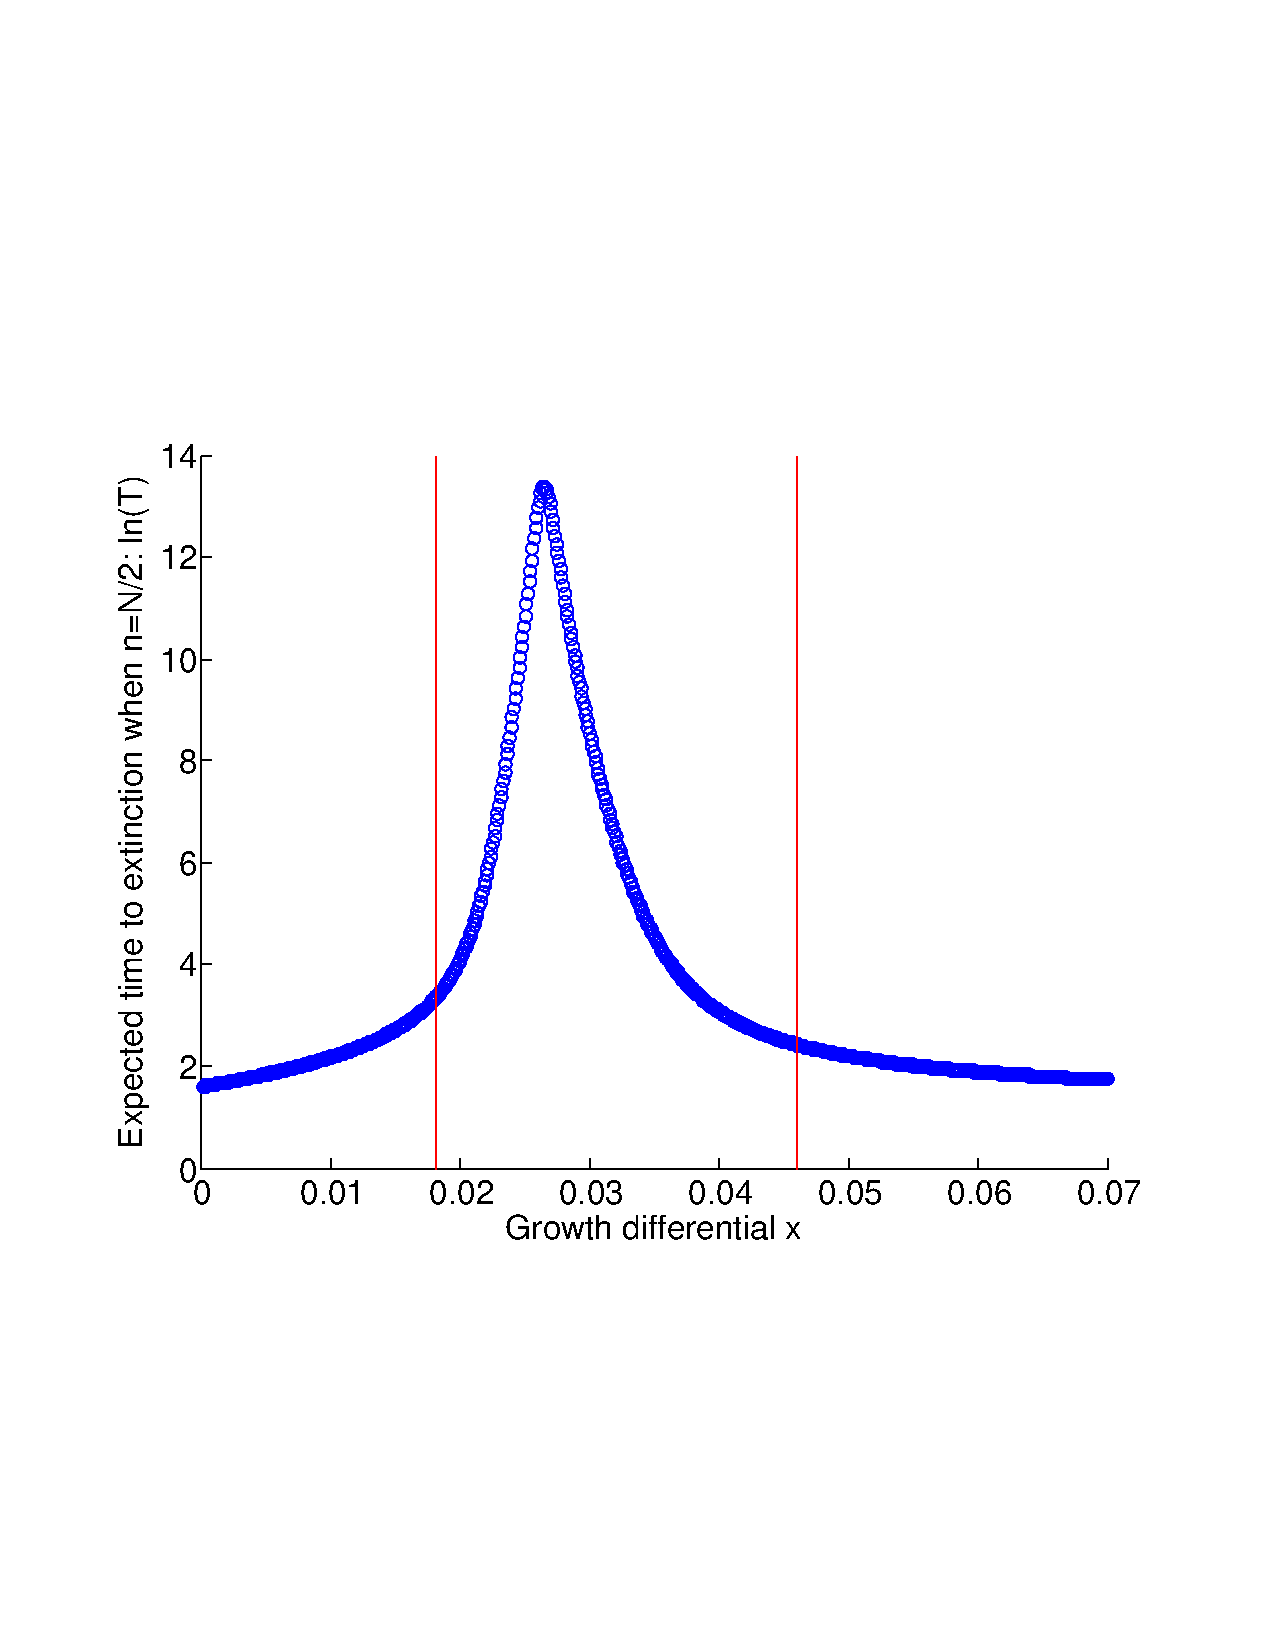
\includegraphics[width=4in]{ttevx.pdf}
 \caption[How time to extinction varies with the difference in growth rates]{\textbf{How time to extinction varies with the difference in growth rates:} The difference in growth rates as measured by time available for invasion $x$ effects the expected time to extinction, when measured from initial population $n=N/2$. Vertical lines represent $x_{min},x_{max}$, and the region predicted to give coexistence between these lines does display the highest expected time to extinction. Parameters are $s_1=500,s_2=50,N=100$.}
 \label{fig:ttevx}
 \end{figure}
 
 The expected time to extinction of the system can be calculated easily in the case where there is no disturbance. Defining the expected number of time steps taken to go from $n$ individuals of species 1 in an environment where disturbance does not occur to either of the absorbing boundaries ($n=0$ or $n=N$) as $k_n$, we can solve a series of simultaneous equations given by
\begin{equation}
k_n=\begin{cases}
0 & n\in\{0,N\} \\
1+P(\text{Increase}(n))k_{n+1}+P(\text{Stay}(n))k_n+P(\text{Decrease}(n)k_{n-1}) & 1\leq n\leq N-1
\end{cases} \end{equation}
to determine the vector $\mathbf{k}$ of expected extinction time for each possible initial population. This varies with growth rate differential $x$, as demonstrated in Figure~\ref{fig:ttevx}, yet also increases with system capacity $N$, as demonstrated in Figure~\ref{fig:tte}. As system size increases by an order of magnitude, the expected time to extinction increases by a greater ratio. This is especially the case within the range of $x$ that invasion analysis suggests gives two species coexistence. Here, increasing the system size from 100 to 1000 causes the expected time to extinction to increase by approximately 12 orders of magnitude.

\begin{figure}[th]
\centering
   \begin{tabular}{rr}
  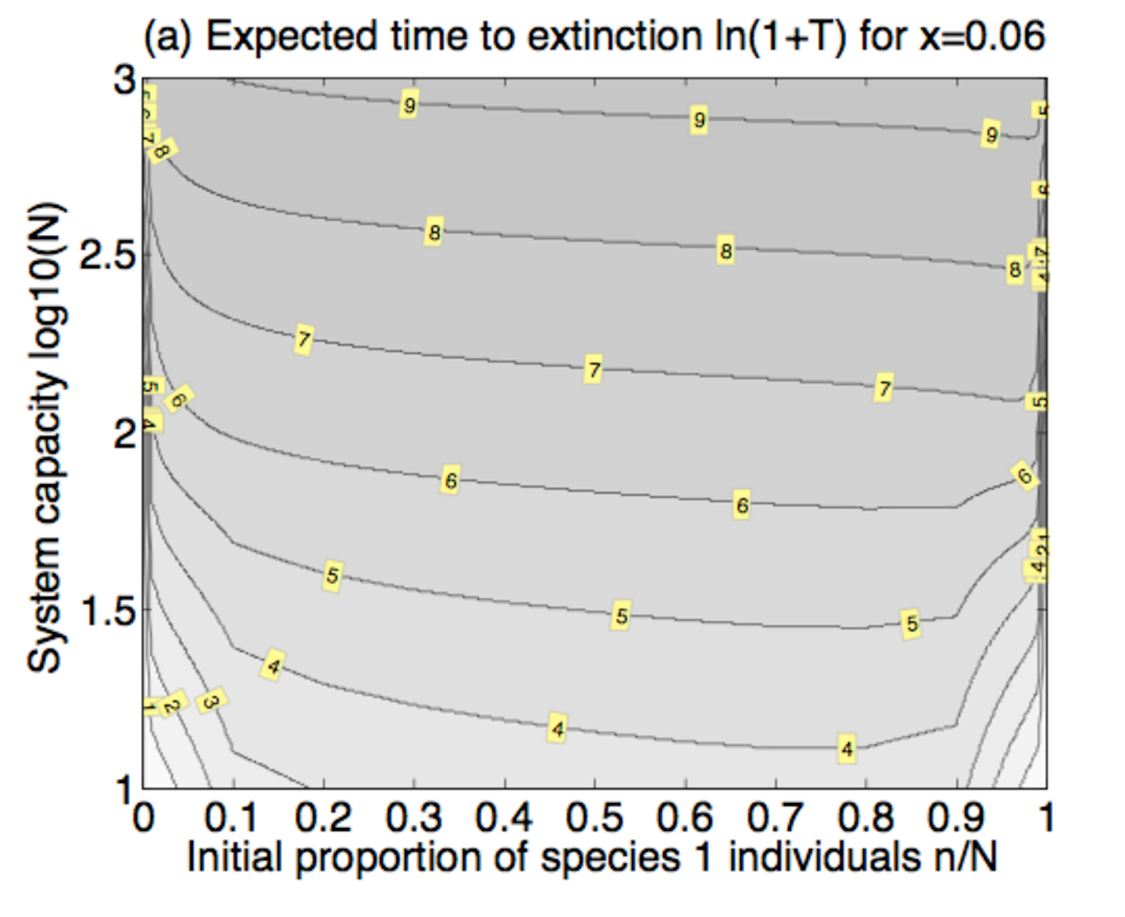
\includegraphics[width=2.5in]{x06resize.pdf} & 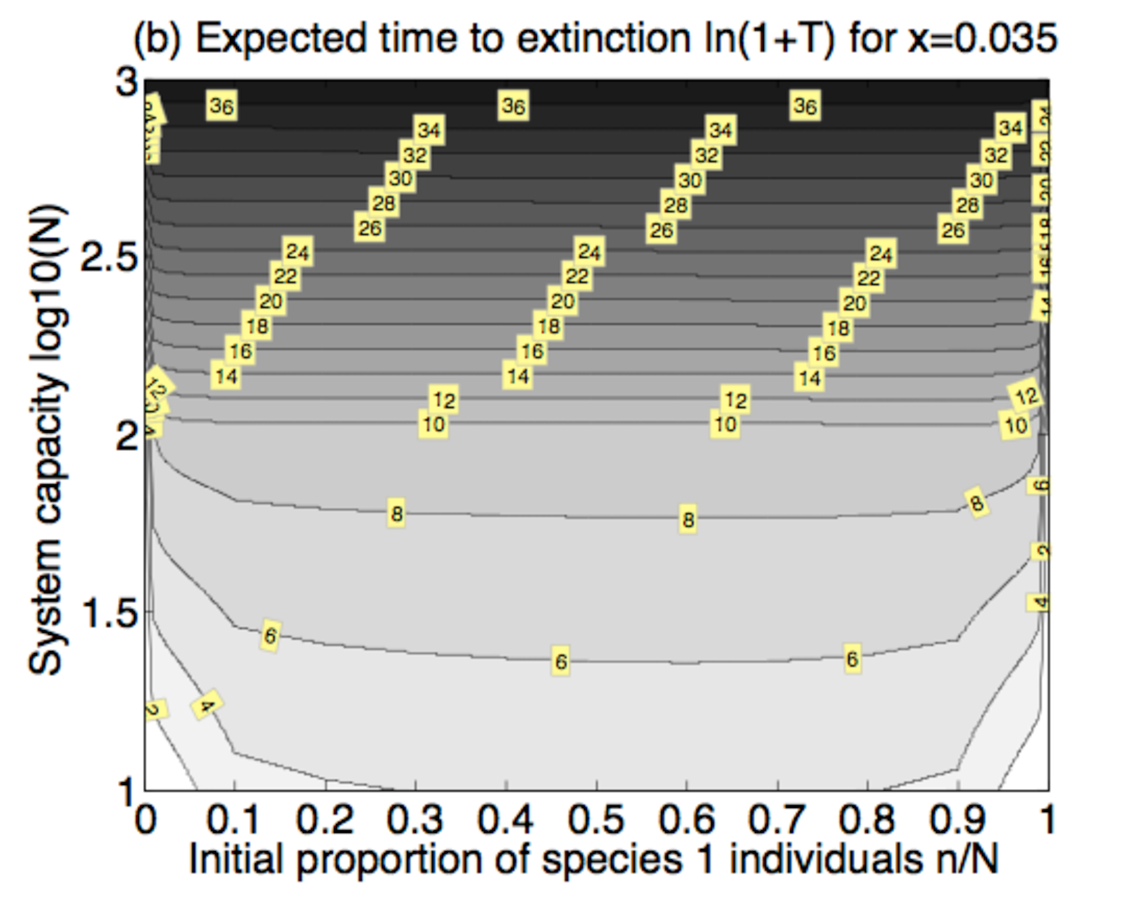
\includegraphics[width=2.5in]{x035resize.pdf} \\
  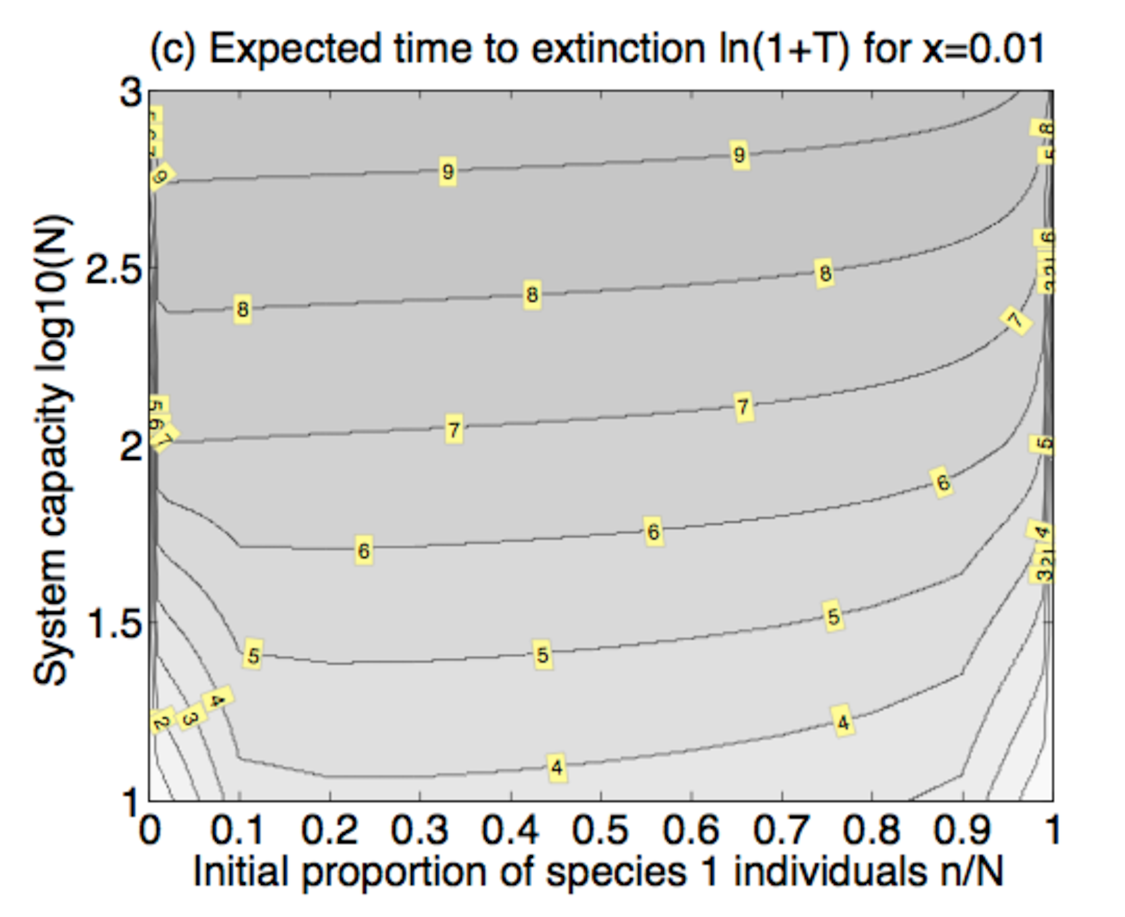
\includegraphics[width=2.5in]{x01resize.pdf} & 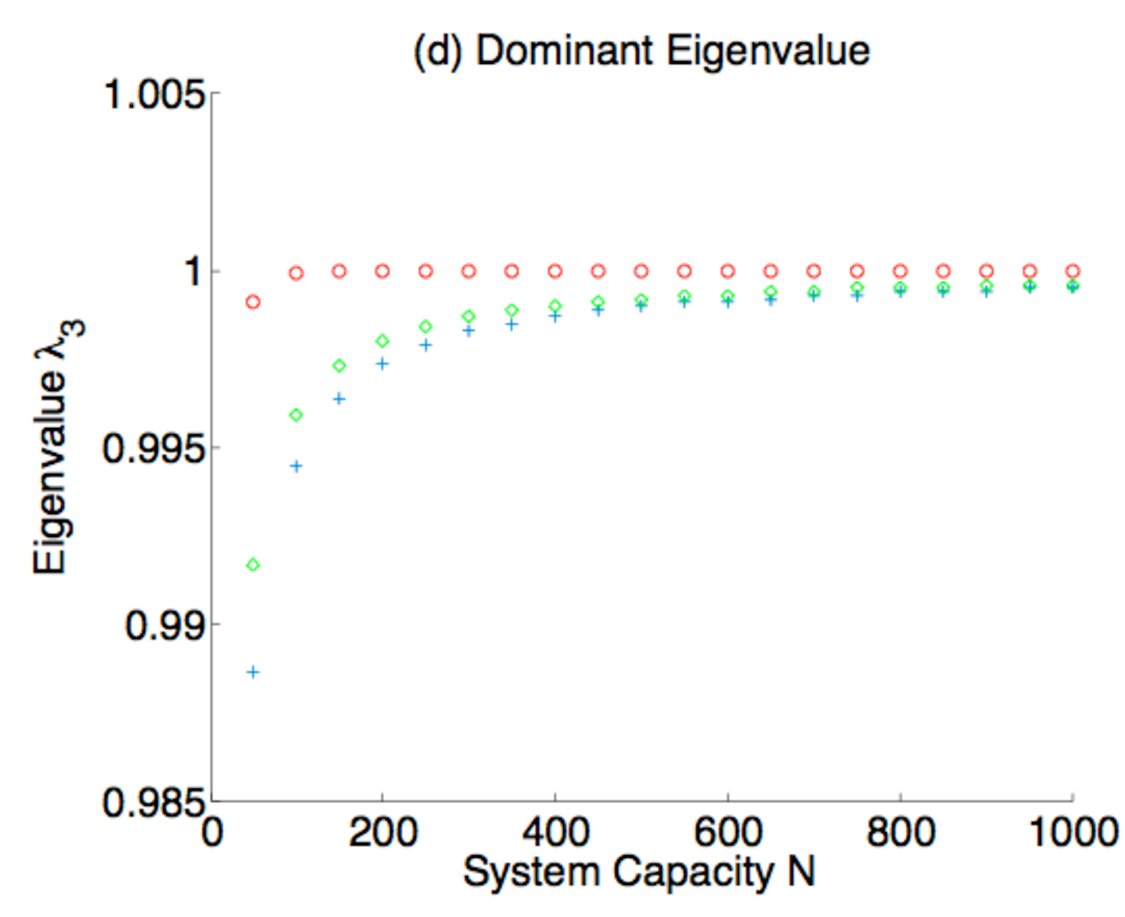
\includegraphics[width=2.5in]{domevalresize.pdf} \end{tabular}
   \caption[How time to extinction varies with system capacity]{\textbf{How time to extinction varies with system capacity: }(a-c) The expected time to extinction as it changes with system capacity $N$ for each initial population. In the region where invasion analysis suggests coexistence should occur, the increase in expected time to extinction with $N$ is greatest, although for all $x$, the increase is more rapid than the increase in system capacity. (d) The effect of system size on dominant eigenvalue $\lambda_3$ for $x>x_{max}$ (crosses), $x<x_{min}$ (diamonds) and $x \in(x_{min},x_{max})$ (circles). Growth rate when the system is away from the boundaries behaves like $\lambda_3^t$. As system capacity increases, $\lambda_3$ tends to 1, resulting in slower convergence to either the boundary or an interior quasi-equilibrium. Note that when $x \in (x_{min},x_{max}$, the convergence $\lambda_3 \to 1$ ccurs more rapidly than for $x$ outside this interval.}
 \label{fig:tte}
\end{figure}

We can also find the expected time to convergence (be that extinction or an internal quasi-equilibrium) by examining the eigenvalues of the transition matrix. The two absorbing boundaries mean that this matrix is reducible, with two eigenvalues $\lambda_{1,2}=1$, so the dynamics away from these boundaries are determined by $\lambda_3$, the largest eigenvalue with $\lambda \neq 1$. The convergence to either the boundary or the quasi-equilibrium happens with rate $\lambda_3^t$. Figure~\ref{fig:tte} shows numerically generated $\lambda_3$ for varied $x \in \{0.01,0.035,0.06\}$ above, below and within the non-disturbed coexistence region. In all cases, $\lambda^3$ increases monotonically with $N$. This indicates that time to convergence increases with system size. When $x \not\in (x_{min},x_{max})$, this extends the time to extinction, allowing for less frequent disturbances to sustain both populations.



 \section{Differential seed productivity}
\label{app2c}
Suppose that not all individuals are reproductively active all the time. Instead, there is a probability  $p$ that an individual is producing seeds at that moment. This effectively reduces the amount of competition for a gap when one appears in the canopy.

We then consider the conditions for coexistence, i.e. \eqref{lowerboundarycond} and \eqref{upperboundarycond}.
We assume that when the system is almost entirely filled with one species, the seed production can be approximated by the mean, so in \eqref{lowerboundarycond} we assume the number of seeds produced by $N-2$ individuals of species 2 is given by $s_2 p (N-2)$. We can therefore solve \eqref{lowerboundarycond} for $x$. Note that a single individual of species 1 can produce either $s_1$ seeds (with probability $p$) or 0 seeds  (probability $1-p$). Using the relationship $P(A)=\sum_{b \in B}P(A|b)$, where $P(A)$ is the probability of species 1 increasing from one individual to two, and $B$ is the of all possible seed numbers produced by species 1 (here the set $\{ 0, s_1\}$), solving \eqref{lowerboundarycond} gives 
\begin{align*}
\ln \left( \frac{(N-1)ps_1}{s_1+ps_2(N-2)}\right) \frac{N}{ps_2(N-2)} &> x. \\
\end{align*}
Taking the limit as system capacity $N$ tends to infinity, we find that an upper bound for $x$ is given by
$$
x<\frac{\ln \left(\frac{s_1}{s_2}\right)}{p s_2}
$$
which merely differs by a factor of $1/p$ from the simpler base model.

Similarly, we can solve \eqref{upperboundarycond} for $x$ as follows:
\begin{align*}
 x&>\frac{N}{s_2}\ln \left( \frac{p^2 s_1(N-1)(N-2)}{((N-1)p-1)(ps_1(N-2)+s_2)} \right) \end{align*}

Again, taking the limit as system capacity $N\rightarrow \infty$ gives 
$$
x>\frac{s_1-s_2}{ps_1s_2}=\frac{1}{p}\left(\frac{1}{s_2}-\frac{1}{s_1}\right) $$
which again differs from the base model merely by a factor of $1/p$. Simulations confirm that between these boundaries, long term coexistence is observed.

\section{Comparison of simulation data with analytic predictions}
\label{app2d}
We ran a range of time series simulations to verify the predictions given by our analytical results. Simulations are run at $I=0.1,0.2,0.3,0.4,0.5,0.6,0.7,0.8,0.9$ and $1$ and frequencies $\ln(T_D)=1,2,3,4,5,6,7,8$. Each point has 20 simulations run for $10^5$ time steps, and a linear interpolation algorithm is used between data points. Dark colours in Figure~\ref{fig:simulationdata}(a) are indicative of high probability of coexistence, where both species persist in the community after $10^5$ time steps. The scale to the right shows the percentage of the 20 time series exhibit coexistence. This data indicates that while the outcomes are accurately predicted by the analysis when disturbance events are very frequent (Figure~\ref{fig:simulationdata}(b)), there is a ``tail'' at high intensity and intermediate frequency where coexistence is only possible for a very narrow range of frequencies. However, frequencies that are sufficiently high (such that the lines given by $\text{AverageChange}(1)=0$ and $\text{AverageChange}(N-1)=0$  are approximately constant in $\ln(T_D)$) the average change function provides a good fit to the simulation data (Figure~\ref{fig:simulationdata}). This is also the case for simulations in a system of size $N=10000$, where the average change provides a good fit for frequencies where the region of coexistence is approximately constant in $f$ (results not shown).
\begin{figure}\begin{tabular}{ll}
(a)&(b)\\
 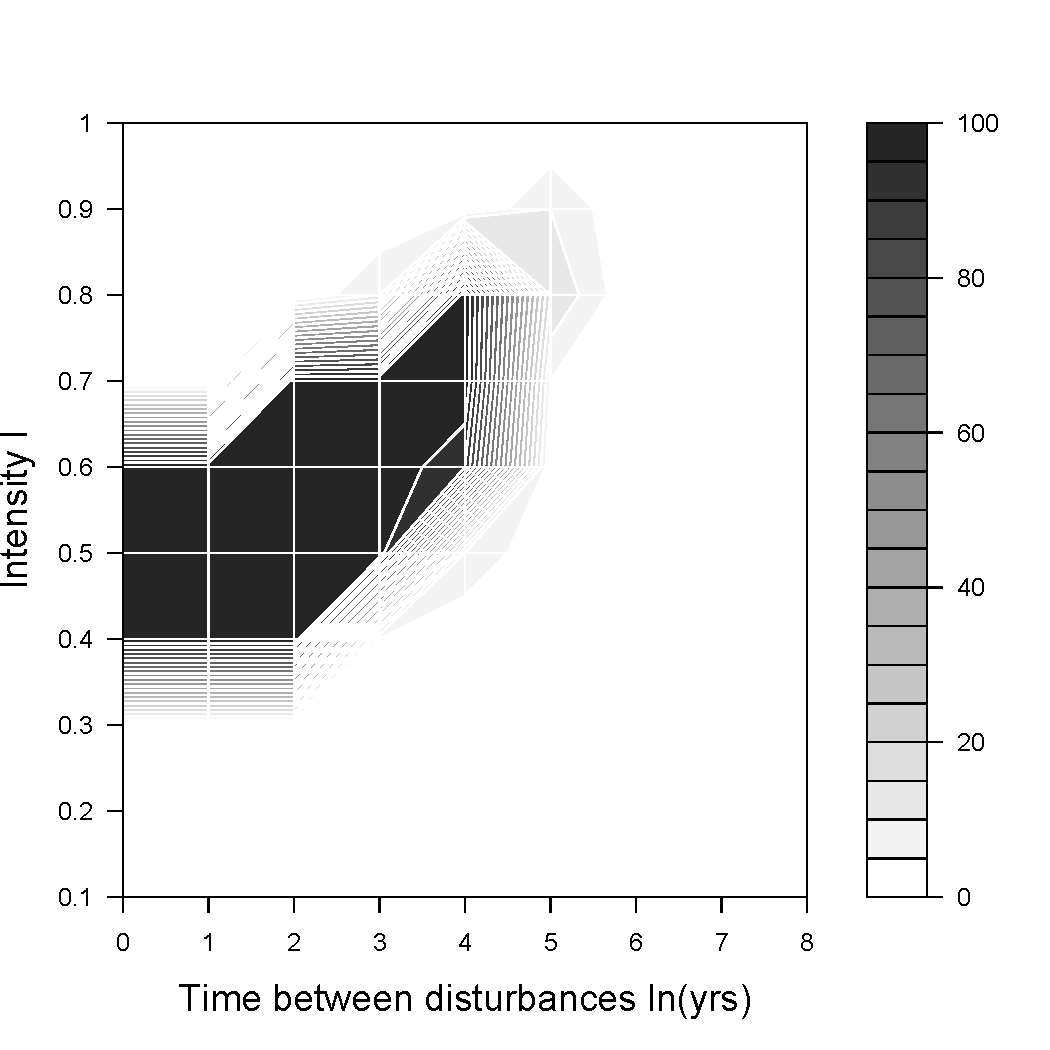
\includegraphics[width=2.5in]{simcoexist.pdf}& 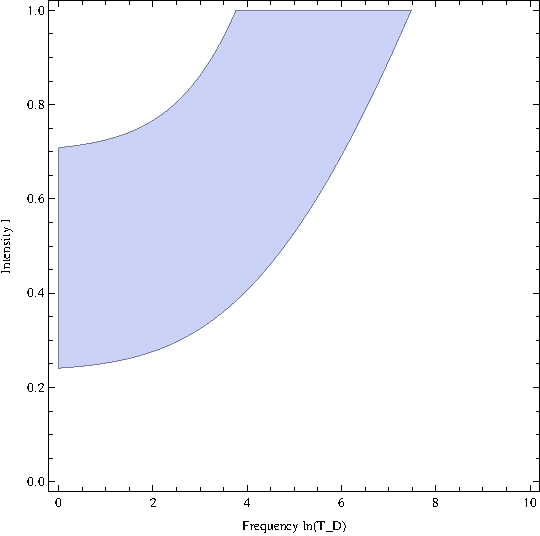
\includegraphics[width=2.5in]{hockeyTd.pdf}\end{tabular}
   \caption[Comparing simulation data with analytical predictions]{\textbf{Comparing simulation data with analytical predictions:} (a) Simulation data showing how stochasticity effects the predicted region of coexistence at high intensity. 20 time series simulations were run for each point. The darker the shading, the greater the number of these time series that exhibited coexistence after $10^5$ time steps. Linear scaling is performed between data points. (b) The region of coexistence predicted by invasion analysis. Parameters $s_1=500,s_2=50,x=0.06,N=1000$}
 \label{fig:simulationdata}
\end{figure}

\section{Approximation of expected change for $p<1$}
\label{app2e}
When not all individuals are reproductively active ($p<1$), the average change at the boundaries is given by
\begin{align}
\label{acd1}
&AvChangeDist(1)=-I \\ 
&+ (1-I)p \notag \\
& \times \sum_{k=0}^{N-2} k \sum_{j=k}^{N-2} I^j(1-I)^{N-2-j}{N-2\choose j} \sum_{r_2=0}^{N-1j} \notag \\
&\left( p^{r_2}(1-p)^{N-1-j-r_2} {N-1-j\choose r_2}\left( \frac{s_1 e^{-s_2xr_2/N}}{s_1+s_2r_2}\right)^k \left(1- \frac{s_1 e^{-s_2xr_2/N}}{s_1+s_2r_2}\right)^{j-k}{j\choose k} \right) \notag \\
&+(N-1)I^{N-1}(1-I) \notag
\end{align}
and
\begin{align}
\label{acdt}
&AvChangeDist(N-1)=-(N-1)I^{N-1}\\& - (1-I)p \notag \\
&\times \sum_{k=1}^{N-2}k\sum_{j=k}^{N-2} I^j(1-I)^{N-2-j} {N-2 \choose j} \sum_{r_1=0}^{N-1-j} \notag \\
&\left( p^{r_1}(1-p)^{N-1-j-r_1} {N-1-j\choose r_1}\left( \frac{s_1r_1 e^{-s_2x/N}}{s_2+s_1r_1}\right)^{j-k} \left(1- \frac{s_1r_1 e^{-s_2x/N}}{s_2+s_1r_1}\right)^k{j\choose k} \right) \notag \\
&+I(1-I^{N-1}) \notag
\end{align}
However, these are computationally expensive, where the number of terms in the triple sum scales as $N^3$, so as system size increases, the calculation of \eqref{acd1} and \eqref{acdt} rapidly becomes unfeasible. Instead, we use the normal approximation of the binomial distributions using the `integral2' function in Matlab2012b, to approximate the expected changes at the boundaries with 
\begin{align}
& AvChangeDistApprox(1)=-I \\
&+(1-I)p \notag \\
&\sum_{k=1}^{N-2} k \int_k^{N-2}dj\quad \mathcal{N}\left(I(N-2),I(N-2)(1-I),j\right) \int_0^{N-1-j}dr_2\quad \mathcal{N}\left(p(N-1-j),p(1-p)(N-1-j),r_2\right) \notag \\
&\times \mathcal{N}\left(j\frac{s_1 e^{-s_2xr_2/N}}{s_1+s_2r_2},j\frac{s_1 e^{-s_2xr_2/N}}{s_1+s_2r_2}\left(1-\frac{s_1 e^{-s_2xr_2/N}}{s_1+s_2r_2}\right),k \right)\notag \\
 &+(N-1)I^{N-1}(1-I)\notag
\end{align}
at the lower boundary and 
\begin{align}
& AvChangeDistApprox(N-1)=-(N-1)I^{N-1}\\
& - (1-I)p \notag \\
& \sum_{k=1}^{N-2}k \int_k^{N-2}dj\quad \mathcal{N}(I(N-2),I(1-I)(N-2),j)\int_0^{N-1-j}dr_1\quad \mathcal{N}(p(N-1-j),p(1-p)(N-1-j),r_1) \notag \\
& \times \mathcal{N}\left(j\left(1-\frac{s_1r_1 e^{-s_2x/N}}{s_2+s_1r_1}\right),j\frac{s_1r_1 e^{-s_2x/N}}{s_2+s_1r_1}\left(1-\frac{s_1r_1 e^{-s_2x/N}}{s_2+s_1r_1}\right)\right) \notag \\
&+I(1-I^{N-1})\notag \end{align}
at the upper boundary, where $\mathcal{N}(x,y,z)$ is the PDF of a normal distribution with mean $\mu=x$ and variance $\sigma^2=y$, analysed over the variable $z$.

The error for this approximation decreases with increased system capacity $N$. Evaluating for $I=0.1,0.2,...,0.9$ and $\ln(T_D)=1,2,...,8$, we find that the maximum error when $N=400$ is 0.0025, ensuring that even for relatively small $N>400$, this is a good approximation of the expected change.



\eappendix


\newpage
\chapter{Which trade-off contributes most to biodiversity? A comparison of trade-off models}
\newpage
\topskip0pt
\vspace*{\fill}
\section*{Abstract}
Trade-offs are considered an important driver of species richness, as trade-offs between life history traits allow for niche specialisation. Plant communities are thought to have three important life history traits; fecundity, juvenile growth and defence against herbivores and/or abiotic pressures. We build upon the model presented in Chapter~2 to consider a variety of trade-offs in an environment that experiences disturbance events of varying intensity and frequency. Using invasion analysis, we enumerate the likelihood of each of these trade-offs allowing to species to coexist, and find that trade-offs between all three traits are most likely to promote coexistence, although this trade-off does not exhibit a significantly greater likelihood of coexistence than a fecundity-growth trade-off. Further, we demonstrate that trade-offs involving growth rate differences are robust to changes in community size, while a fecundity-defence trade-off cannot sustain more than a single species in large communities. 
\vspace*{\fill}
\newpage

\section{Introduction}
No single species can allocate unlimited resources to each life history trait \citep{law1979optimal,tilman1982resource}. Instead, species life histories are determined by the allocation of limited resources to different areas of need. In plant species, the three important life history traits are reproduction, growth from seedling to adult, and defence against both herbivory and abiotic factors such as fire \citep{bazzaz1987allocating}. This leads to trade-offs between life history traits. For example, a species with high levels of resource allocated to increasing fecundity will not be able produce seeds of a large mass \citep{turnbull1999seed} and, since seed size is positively correlated with juvenile growth rate, is therefore likely to experience a decrease in its juvenile growth rate \citep{gross1984effects}, or a species with rapid growth may be more susceptible to damage by storm winds or other mortality pressures such as large scale herbivory \citep[e.g.][]{wright2010functional,fine2006growth}. Theory has shown that these trade-offs can allow two or more species to coexist while competing for  the same resources in an environment \citep[e.g.][]{kisdi2003coexistence,levins1971regional,bonsall2004life}, suggesting that trade-offs are important for sustaining high levels of biodiversity in nature. However, while some studies have compared several trade-offs \citep[e.g.][]{tilman1990constraints,grime1977evidence}, little is understood about how multiple trade-offs combine to affect community diversity, and whether trade-offs on multiple axes increase diversity in an additive manner.

Conditions under which species coexist alongside others will also be dependent on other, abiotic factors. \textbf{For example, during a hurricane, some tree species experience high stem breakage and mortality, while others suffer much lower mortality \citep{zimmerman1994responses}. This is caused by increased wood density, which correlates with breaking strength \citep{niklas1992plant}. Wood density is also negatively correlated with growth rates \citep{king2005tree}, suggesting that trade-offs between growth, defence against rare disturbance events and fecundity may be complex. Understanding how these trade-offs interact is potentially crucial in understanding how diversity is maintained.}

Several previous studies have suggested that disturbance events also play an important role in promoting and maintaining diversity \citep[e.g.][]{sousa1984role,denslow1987tropical}.  Recent theoretical work \citep[Chapter~1;][]{miller2011frequency,nattrass2012quantifying} shows that different measures of disturbance, such as frequency or intensity, will have very different effects, even when the total biomass lost to disturbance over a given time period is taken into account. While many empirical studies consider disturbance as a single parameter \citep[e.g.][]{molino2001tree,peterson1997tornado,nakagawa2000impact}, some studies do demonstrate that different factors determining disturbance can affect the community structure differently. \cite{hall2012diversity} use bacterial populations to experimentally demonstrate that the frequency and intensity of disturbance events have different impacts, while \cite{denslow1980patterns} indicates that communities with large, infrequent disturbances may be more diverse than those where disturbance events are more frequent, yet clear a smaller area (e.g. tree-fall gaps).

Here, all possible trade-offs between the three important plant life history traits - reproduction, juvenile growth and defence - are considered in a two species model. Defence is taken here to mean the ability of an individual to withstand a disturbance event, that is, an event that results in the death of large number of individuals and alters niche opportunities within the community, while seed production (seed number per capita per year) is used as the measure of fecundity. We therefore consider 8 models. The model where all species are identical gives neutral dynamics, and the coexistence of the two species is governed by chance, while the three models where the species differ in a single trait (no trade-off) demonstrate competitive exclusion of the weaker species. When trade-offs are between two or more traits, the effects of system capacity and varied disturbance regimes  are considered, and we show that trade-offs between fecundity and growth, or growth and defence, can support two species for large system sizes, as can a three dimensional trade-off, although a fecundity-defence trade-off cannot. The probability of species disturbance defence parameters resulting in coexistence is calculated, and we demonstrate that a three dimensional trade-off gives the greatest likelihood of coexistence, an order of magnitude larger than that of a growth-defence trade-off. Species specific disturbance intensities are then linked to allow comparison between the three dimensional trade-off and a fecundity-growth trade-off, allowing us to test whether increasing the number of trade-off axes has a significant effect on diversity. When disturbance affects all species equally, we show that if the more fecund of the two species has a slight advantage in defence against disturbance, the likelihood of coexistence is maximised, although this increase is marginal.


\section{Models}
Here, we build on the model presented in Chapter 2, introducing a single extra factor; we allow species to differ in the level of resource they dedicate towards resistance to disturbance events, so an individual of species $i$ will experience a species specific probability of death during a disturbance $I_i$. The model is described in a non disturbance time  step by the following transition probabilities (where $n=N_1(t)$ and $N-n=N_2(t)$);
\begin{align}
\label{inc}P(\text{increase}(n))=&\frac{N-n}{N}\frac{s_1 n}{s_1 n +s_2(N-n-1)}\exp \left( -s_2 \frac{N-n-1}{N} x\right),\\
\label{dec}P(\text{decrease}(n))=&\frac{n}{N}\frac{s_2 (N-n)}{s_1 (n-1) +s_2(N-n)}  \\
& + \frac{n}{N}\frac{s_1 (n-1)}{s_1 (n-1) +s_2(N-n)}\left(1-\exp \left( -s_2 \frac{N-n}{N} x\right)\right), \notag \\
\label{stay}P(\text{stay}(n))=&1-P(\text{increase}(n))-P(\text{decrease}(n)).
\end{align}
where $s_i$ is the per capita annual seed production of species $i$, $N$ is the system capacity - the maximum number of adults that can be sustained by the environment, and $x=C(1/g_1 - 1/g_2)/2$ is a measure of growth rate differences (with $C$ canopy height and $g_i$ the sapling growth rate of species $i$).

During a disturbance event, each individual of species $i$ will die with probability $I_i$. If there are $d_i$ deaths of species $i$, then the total deaths is given by $d=\sum_i d_i$. Note that $d$ is now dependent on the species composition of the community when the disturbance strikes, as well as the inherent properties of the disturbance. The expected number of deaths is given by
\begin{equation}
\label{avdeaths} \bar{d}=\sum_i I_i N_i(t)
\end{equation}
where $N_i(t)$ is the population of species $i$ at time $t$. Once all $d$ deaths occur, the remaining $N-d$ individuals compete for the opened sites in the system. If the populations of the two species are given by $n_1^*,n_2^*$ in the immediate aftermath of a disturbance, the probability of each gap being successfully colonised by species one is given by
\begin{equation}
\label{sp1c3}
Sp_1(n_1^*,n_2^*)=\frac{s_1 n_1^*}{s_1n_1^*+s_2n_2^*}\exp \left(-s_2 x\frac{n_2^*}{N}\right).
\end{equation}

We assess coexistence by considering invasion analysis. The average or expected change in a time step is approximated by
\begin{align}
\label{ac}
\text{AverageChange}(n)=&(1-f)\left(P(\text{increase}(n))-P(\text{decrease}(n))\right)  \\
&+f\left(-nI_1 +(nI_1+(N-n)I_2)Sp_1(n(1-I_1),(N-n)(1-I_2))\right).\notag
\end{align}
This approximation does not account for Jensen's inequality, yet Appendix~\ref{appapproximations} shows that for each of the models considered, the approximation at the boundaries $(n=1,N-1)$ improves with system capacity $N$, and fits the actual expected change well. Coexistence occurs when on average, both species increase when rare; that is when
\begin{align}
\label{avch1}\text{AverageChange}(1)&>0,\\
\label{avchn-1}\text{AverageChange}(N-1)&<0. \end{align}

We can now consider a collection of models by varying different combinations of the three traits; fecundity, juvenile growth rate and defence or resistance to disturbance, using the parameter values shown in Table~\ref{tabparas}. This gives a selection of 8 models, one where the species are identical, 3 where they differ in a single parameter, 3 where they differ in two ways and the third parameter is equal, and a final model where species can differ in all three ways. The first four of these are trivial to analyse, but the models where species differ in at least two of the life history parameters give more interesting results.

\begin{table}[htdp]
\begin{center}
\begin{tabular}{|c|l|c|} \hline
\multicolumn{3}{|c|}{Table of baseline parameters} \\ \hline
Parameter & Description & Default value \\ \hline
$s_1$ & per capita annual seed production of species 1 & 500 \\ \hline
$s_2$ & per capita annual seed production of species 2 & 50\\ \hline
$g_1$&growth rate of species 1 juveniles & 13 \\
&(measured in mm/yr for diameter at breast height) &\\ \hline
$g_2$&growth rate of species 2 juveniles & 13.21 \\
&(measured in mm/yr for diameter at breast height) &\\ \hline
$C$& size of individuals at canopy height & 100 \\
& (measured in mm for diameter at breast height&\\ \hline
$x$&$C(1/g_1-1/g_2)/2$&0.06\\
&time window (yrs) for successful secondary colonisation by species 2&\\ \hline
$N$ & system capacity: number of individuals the region can support & 1000 \\ \hline
$n$ & number of species 1 individuals & N/A \\ \hline
$T_D$& average time between disturbances in yrs & 10 \\ \hline
$f$& within event disturbance probability & $100/(T_D N)$ \\ \hline
$I_1$& intensity of disturbance for species 1 & N/A \\ \hline
$I_2$& intensity of disturbance for species 2 & N/A \\ \hline
$y$ &Parameter linking species intensities; given by $I_1/I_2$ & N/A \\ \hline
\end{tabular} \end{center}
\caption[Key model parameters]{Key parameters used in the model, along with default values where appropriate}
\label{tabparas} 
\end{table}

\section{Results}
When all species are identical, the model is simply a one-dimensional random walk, where disturbance events of intensity $I$ merely increase the distance it is possible to travel in a single step. Coexistence in this model is merely a function of chance. This model therefore acts as a neutral theory model without mutation or speciation, where all species are equivalent and chance alone drives dynamics. If the species merely differ in a single parameter, then we find that the species with the higher growth rate or fecundity, or with the lower mortality in a disturbance regime will competitively exclude the other.

\subsection{Fecundity-growth trade-off}
The case where species differ in both fecundity and growth ($I=I_1=I_2$) is analysed in detail in Chapter 2. In summary, for sufficiently low growth rate differentials $x$,  the more fecund species 1 can competitively exclude the rapidly growing species 2, both in the presence of disturbance and in an environment without disturbance. For intermediate $x$, coexistence is possible in the homogeneous environment, and this behaviour persists for low intensity or low frequency disturbances. As disturbance intensity increases (providing the frequency $f$ is greater than the expected time to extinction $t_{extinct}$), the fecundity advantage of species 1 will lead to it competitively excluding species 2. Thus, disturbance can lead to a decrease in diversity. When $x>x_{max}$ is large, species 2 will exclude the more fecund species 1 due to its superior growth rate. In this case, disturbance has a more complex effect. For frequencies $f$ such that $1/f > t_{extinct}$, intermediate disturbances will lead to coexistence of two species, while high intensities will allow the previously excluded species 1 to claim all sites and exclude species 2. Low intensities are insufficient to change the temporally homogeneous diversity, although may extend the time to coexistence. When $1/f < t_{extinct}$, species 2 will persist in monoculture. System size impacts the region of coexistence by increasing $t_{extinct}$, extending the region of more complex behaviour.

For a large system, or disturbances more frequent that $t_{extinct}$, the range of intensities that can give coexistence varies with the growth rate differential $x$, and is maximised at $x=x_{max}$, and also with the difference in fecundities. As seed numbers are varied, the maximum range of disturbance is at the point $s_1=s_2\exp(s_2x)$. That is, the range is maximised when the function $I=1-\ln(s_1/s_2)/(s_2x)$, formed by setting $\text{AverageChange}(1)=0$, returns $I=0$.

\subsection{Fecundity-defence trade-off}
When species have identical growth rates ($x=0$), yet differ in disturbance response and fecundities $s_i$, it is possible to find analytically the range of $I_1 - I_2$ space that gives coexistence for given fecundities $s_i$. We define $A(n)=(1-f)(P(\text{increase}(n))-P(\text{decrease}(n)))$, which is independent of $I_2$. Setting $\text{AverageChange}(1)=0$ and solving for $I_1$ gives
\begin{align}
\label{fdac1sol}
I_1=&\frac{I_2(f(N-1)s_1-A(1)s_2(N-1)) +A(1)(s_1+s_2(N-1))}{I_2f(N-1)(s_1-s_2) +fs_2(N-1) +A(1)s_1}\notag \\
=&\frac{\alpha_1 I_2 +\beta_1}{\gamma_1 I_2+\delta_1}
\end{align}
while setting $\text{AverageChange}(N-1)=0$ gives the curve
\begin{align}
\label{fdacnsol}
I_1=&\frac{I_2(f(N-1)s_1-A(N-1)s_2) +A(N-1)(s_1(N-1)+s_2)}{I_2f(N-1)(s_1-s_2) +fs_2(N-1) +A(N-1)s_1(N-1)}\notag \\
=&\frac{\alpha_{N-1} I_2 +\beta_{N-1}}{\gamma_{N-1} I_2+\delta_{N-1}}
\end{align}
where
\begin{align}
\alpha_i =& f(N-1)s_1 - A(i) s_2 (N-i), \notag \\
\beta_i =& A(i) (s_1 i + s_2(N-i)), \notag \\
\gamma_i =& f(N-1)(s_1-s_2), \notag \\
\delta_i =& fs_2(N-1) + A(i)s_1 i. \notag
\end{align}
The region of coexistence is therefore the area between the two curves, as demonstrated in Figure~\ref{fd}(a). By noting that the indefinite integral of $(a x +b)/(c x +d)$ is $ax/c+(bc-ad)\ln(d+cx)/c^2 +const.$, we can write a formula for the area of the region of $I-$space that predicts coexistence;
\begin{align}
&\min \left(1, \int_0^1 dI_2 \quad \frac{\alpha_1 I_2 +\beta_1}{\gamma_1 I_2+\delta_1} \right) -  \int_0^1 dI_2\quad \frac{\alpha_{N-1} I_2 +\beta_{N-1}}{\gamma_{N-1} I_2+\delta_{N-1}}  \notag \\
=&\min\left(1,\frac{\alpha_1}{\gamma_1}+\frac{(\beta_1 \gamma_1 - \alpha_1 \delta_1)(\ln(\delta_1 +\gamma_1)-\ln(\delta_1)}{\gamma_1^2}\right) \\
&-\frac{\alpha_{N-1}}{\gamma_{N-1}}-\frac{(\beta_{N-1} \gamma_{N-1} - \alpha_{N-1} \delta_{N-1})(\ln(\delta_{N-1} +\gamma_{N-1})-\ln(\delta_{N-1})}{\gamma_{N-1}^2}. \notag
\end{align}
The minimum is taken in the first term because for sufficiently large $s_1$, the function given by \eqref{fdac1sol} is greater than one for all $I_2 \in (0,1)$, but an intensity of greater than 1 is impossible. When
\begin{equation}
\label{fdto:lbint}
\int_0^1 dI_2 \quad \frac{\alpha_1 I_2 +\beta_1}{\gamma_1 I_2+\delta_1} >1
\end{equation}
the inequality $\text{AverageChange}(1)=0$ is satisfied for all possible combinations of disturbance defence parameters $I_1,I_2$. Therefore, the area of the region of $I-$space satisfying {avch1} is equal to the size of the whole region, 1. This minimum is not necessary in the second term, as the integrand
$$
\frac{\alpha_{N-1} I_2 +\beta_{N-1}}{\gamma_{N-1} I_2+\delta_{N-1}}
$$
tends to one from below as $s_1$ increases.
 Hence, the region of coexistence does not change with $s_1$ in a smooth manner, as shown in Figure~\ref{fd}(d). The peak range of coexistence is given by intermediate $s_1=14225$ (for fixed $s_2=50$), with the region area tending to zero as the difference in species fecundities tends to infinity. For the chosen parameters, and system size $N=1000$, the peak probability of coexistence (when intensities for the two species are chosen at random) is approximately 0.120.
\begin{figure}[htbp]
\begin{tabular}{cccc}
(a)&&(b)&\\
&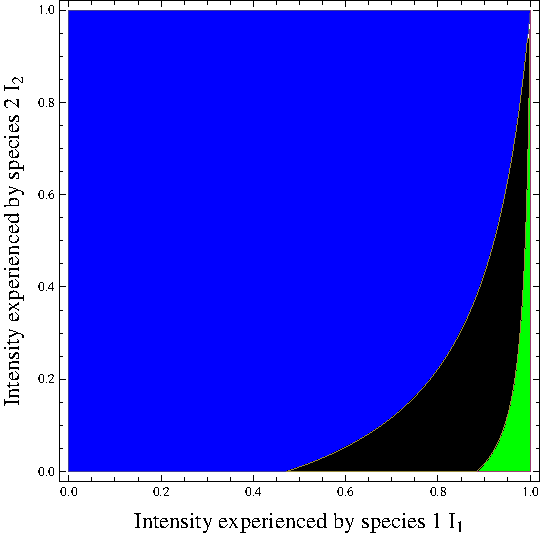
\includegraphics[width=2in]{fdtoexample.pdf}&&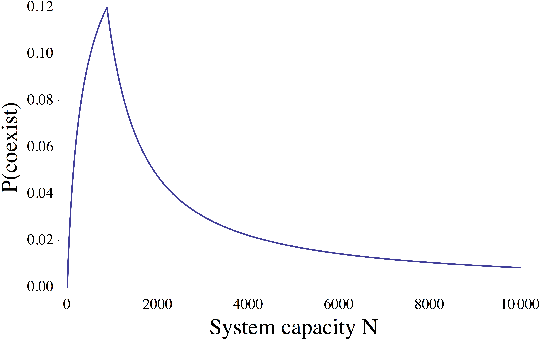
\includegraphics[width=2in]{fdtointwN.pdf} \\
(c)&&(d)&\\
&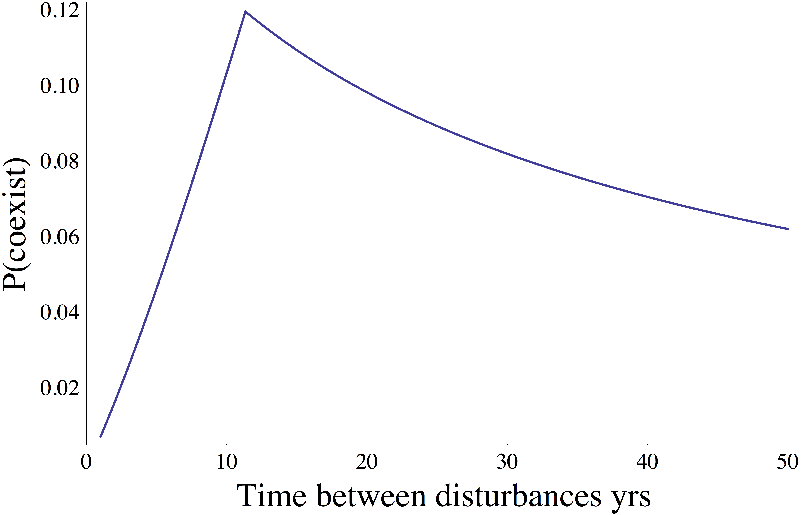
\includegraphics[width=2in]{fdtointwTd.pdf}&&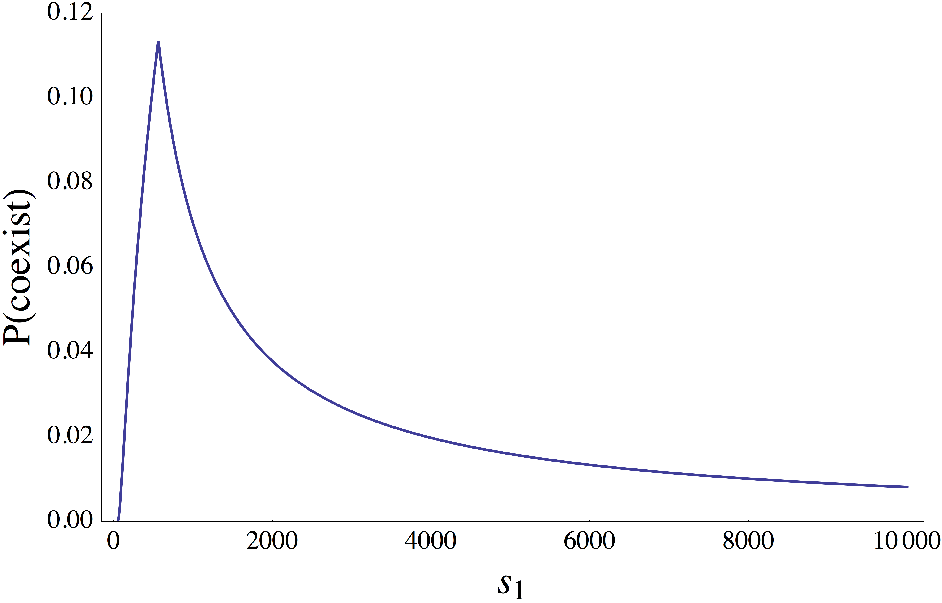
\includegraphics[width=2in]{fdtointws1.pdf}
\end{tabular}
\caption[Consequences of a fecundity-defence trade-off]{\textbf{Fecundity-defence trade-off:} (a) An example of the region of coexistence. The blue area (top and left, dark shading) is where species 1 can invade when rare, while the green area (bottom and right, pale shading) gives the region where species 2 can invade. The region where they overlap (black) is the region that gives coexistence. (b) The effects of changing system capacity on the area of the region of $I-$space that predicts coexistence. The region of coexistence peaks in area at intermediate system capacity $N\approx 850$, and declines with system size above this value. (c) The change in the likelihood of coexistence as time between disturbances $T_D$ is increased. The size of this region is maximised at intermediate values of $T_D \approx 10$, and tends to 0 as $T_D$ goes to infinity. (d) The change in the likelihood of coexistence as $s_1$ is increased. Note the discontinuity where \eqref{fdac1sol} becomes greater than one as $s_1=14225$.  Parameters $s_1=500,s_2=50,N=1000,T_D=10$ unless specified.}
\label{fd}
\end{figure}

Increasing frequency by reducing the expected time between disturbances $T_D$ also has a dramatic effect on the results. For very low frequency, all combinations of defence responses exclude species 2, as the fecundity disadvantage it experiences cannot be overcome. As frequency is increased, then very high $I_1$ can combine with low $I_2$ to give a small region of coexistence. For example, if a species devotes a great deal of resource to surviving fire, it could persist with a species very susceptible to fire but with a greater fecundity. This advantage in fecundity ensures the species is better able to reach empty sites after a disturbance, and is therefore likely to claim sites uncontested by the poorer coloniser. The range of parameters $I_i$ that give coexistence in this way increases with frequency until a threshold is reached (see Figure~\ref{fd}(c)) at which point, it is possible for species 2 to outcompete species 1 if $I_2<<I_1$.

The region of $I-$ space where coexistence is expected then begins to decline in area, as the two curves comprising the boundaries of the region both tend to the curve $I_1=I_2s_1/(I_2s_1+s_2(1-I_2))$ as frequency $f$ tends to one ($T_D \to 0$). In the limit as $f \to 1$ where `disturbance' events are so frequent as to provide an homogeneous environment themselves, both functions given by \eqref{fdac1sol} and \eqref{fdacnsol} are defined by this single curve, and coexistence is not possible. If $I_1>I_2s_1/(I_2s_1+s_2(1-I_2))$ then species 2 will dominate the environment, while if $I_1<I_2s_1/(I_2s_1+s_2(1-I_2))$ species 1 will exclude the less fecund species 2.

As system capacity $N$ increases, the range of coexistence shows a peak at $N \approx 850$. For wood or forest sized systems above this value, the region area will decline rapidly with increased system capacity. When the system capacity tends to infinity, the region of $I-$space giving coexistence tends to zero. A fecundity-defence trade-off cannot sustain two species in a large system, and has little effect in promoting biodiversity when system size reaches that of a forest or wood. The maximal effect on coexistence is restricted to a very small range of parameters, with steep declines in the probability of coexistence when moving away from these optimal parameter values. 

\subsection{Growth-defence trade-off}
A growth-defence trade-off ($s=s_1=s_2=50$) responds to changes in system capacity and frequency in a very different manner to the fecundity-defence trade-off outlined above. Here frequency has little effect provided that $1/f<t_{extinct}$, while if this condition is not satisfied, the faster growing species will exclude its competitor for any disturbance intensity regime. The response to system size is similar to that of the fecundity-growth trade-off: as system capacity increases, the system asymptotes to a fixed region where coexistence is predicted. Setting $\text{AverageChange}(1)=0$ and $\text{AverageChange}(N-1)=0$ gives $I_1$ as quadratic functions of $I_2$, $LBR(I_2), UBR(I_2)$, outlined in Appendix~\ref{approots}.
The solutions presented in Appendix~\ref{approots} are each of the form
$$
\frac{-b\pm \sqrt{b^2-4ac}}{2a}.
$$ 
However, we note that each equation has one solution greater than one for all of the wide range of $x_s$ considered here. The solution given by the positive square root in \eqref{lbr}, and that given by the negative square root in \eqref{ubr} are both above one for all parameters tested. Therefore, these roots do not affect the behaviour of the system. The dynamics of the model are therefore determined by the negative square root in \eqref{lbr} and the positive square root in \eqref{ubr} (see Appendix~\ref{approots}).
\begin{figure}[htbp]
\begin{tabular}{cccc}
(a)&&(b)&\\
&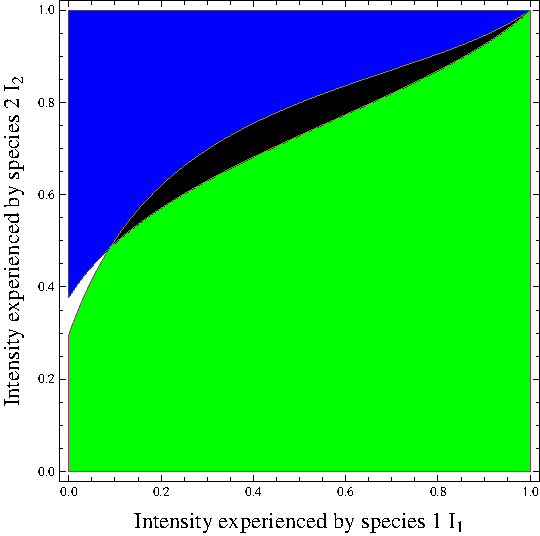
\includegraphics[width=2in]{gdx26.pdf}&&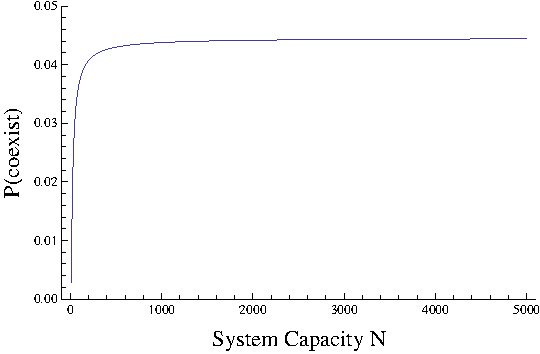
\includegraphics[width=2in]{gdtointwN} \\
(c)&&(d)&\\
&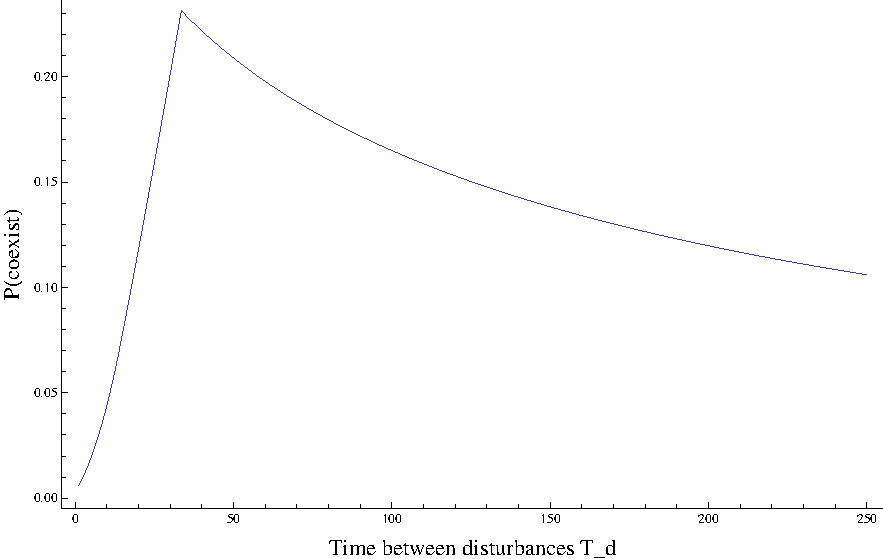
\includegraphics[width=2in]{gdtointwTd}&&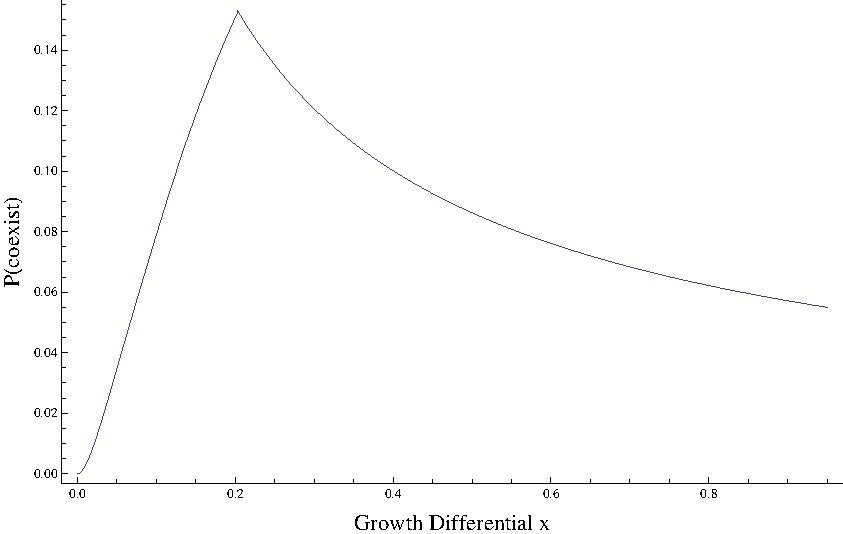
\includegraphics[width=2in]{gdtointwx}
\end{tabular}
\caption[Consequences of a growth-defence trade-off]{\textbf{Growth-defence trade-off:} (a) An example scenario, where coexistence can occur if both species suffer high mortality in a disturbance event. The blue area (top and left, dark shading) is where species 1 can invade when rare, while the green area (bottom and right, pale shading) gives the region where species 2 can invade. The region where they overlap (black) is the region that gives coexistence. The white region exhibits founder control. (b) The effects of changing system capacity $N$ on the likelihood of coexistence. As $N$ increases, the probability of coexistence stabilises as the integral asymptotes to a fixed value. (c) The change in the likelihood of coexistence as time between disturbances $T_D$ is increased. The size of this region is maximised at intermediate values of $T_D \approx 45$, and tends to 0 as $T_D$ goes to infinity. (d) The change in the likelihood of coexistence as $x$ is increased. Note the discontinuity where  the size of the region of coexistence peaks at $x\approx 0.2$. Parameters $s=50,x=0.06,N=1000,T_D=10$ unless specified.}
\label{gd}
\end{figure}
We can numerically integrate to find the area of the region of coexistence, using the following formula:
\begin{equation}
\int_{\max(0,I^*)}^1 dI_2\quad LBR(I_2) - \int_{\max(0,I^*)}^1 dI_2\quad UBR(I_2),
\end{equation}
where $I^*<1$ is the point at which $LBR(I^*)=UBR(I^*)$. This point exists, and is unique, for all parameters tested, although confirming this uniqueness for any parameter choices is beyond the scope of the current work. Note that for all parameters, $LBR(1)=UBR(1)$. This numerical integration allows us to study the behaviour of the system as $x$ is varied. When $x=0$ and the growth rates are identical, the species with the most resistance to disturbance (lowest $I_i$) will exclude its competitor.  As $x$ is increased, four distinct regions will occur, as in Figure~\ref{gd}(a). When both species display high resistance to disturbance (low $I_i$) there is a small region where neither $\text{AverageChange}(1)>0$ or $\text{AverageChange}(N-1)<0$ are satisfied, and founder control occurs, where coexistence does not occur and the successful species depends on the initial populations, subject to stochastic noise. When both species have higher intensities, there exists a region where coexistence is expected. Together the two regions of coexistence and founder control form a band from across $I-$space that separate regions where species and species 2 will exclude the other. We find the region of coexistence peaks at intermediate $x \approx 0.2$, when the probability of two species with randomised defence regimes coexisting is approximately $0.15$. As $x$ increases beyond this, the region of coexistence declines and tend to the region of $I-$space where $I_2>>I_1$, eventually tending to zero as $x$ tends to infinity.

\subsection{Three dimensional trade-off}
When species are allowed to vary in all three traits, fecundity, growth and defence, the region of coexistence is given by integrating the functions \eqref{lbr} and \eqref{ubr}, as determined in Appendix~\ref{approots}. For the three dimensional trade-off, this integral takes the form
\begin{equation}
\int_{\max(0,I^*,I^+)}^1 dI_2 \quad LBR(I_2) - \int_{\max(0,I^*,I^{++})}^1 dI_2 \quad UBR(I_2),
\end{equation}
where $LBR(I^*)=UBR(I^*)$ with $I^*<1$, $LBR(I^+)=0$, and $UBR(I^{++})=0$. For all parameters considered here, these points are well defined and unique. As in the growth-defence case, the roots with the negative square root are those that control the behaviour of the system. Numerically integrating, we can again calculate the region of coexistence in $I-$space. The region of coexistence in $I-$space is shown in Figure~\ref{full}(a). Calculating the areas of coexistence shows that for fixed seed numbers, the area of coexistence will peak at intermediate values of $x$, while for fixed $x$, the range of coexistence will increase as the discrepancy in fecundities becomes more pronounced. This increase will asymptote to the point where it is not possible for species 2 to exclude species 1, but where a significant proportional of trait space will give coexistence (See Figure~\ref{full}(d,f)). The region of coexistence generated by this model is consistently larger than that of the other two models (with $s_1=500,s_2=50,T_D=10,N=1000$, we see that the maximum range of coexistence is given when $x\approx 0.22$, and this region of coexistence has area $\approx 0.271$)
\begin{figure}[htbp]
\centering
\begin{tabular}{rrrr}
(a)&&(b)&\\
&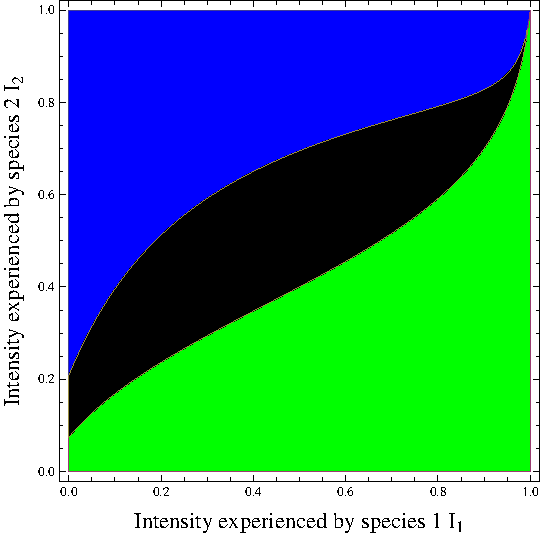
\includegraphics[width=2in]{fullexample.pdf}&&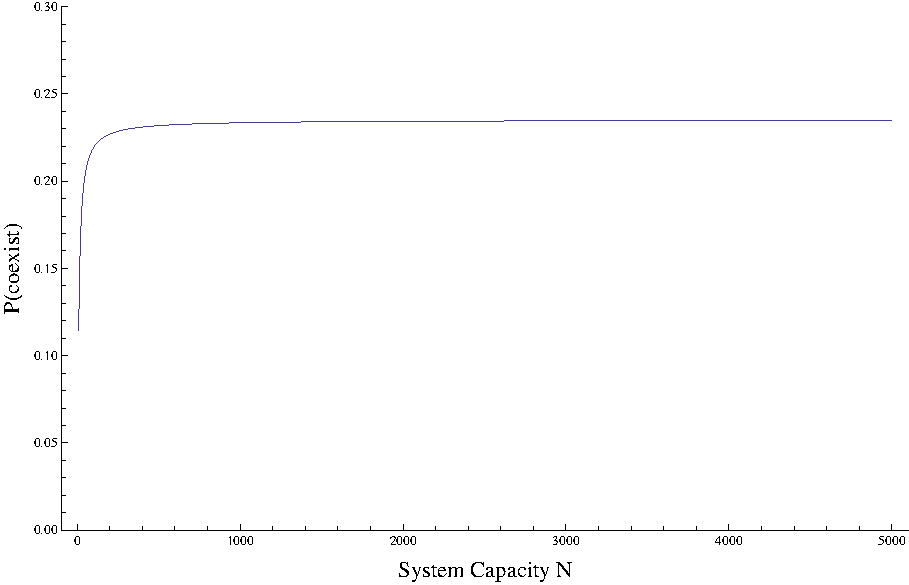
\includegraphics[width=2in]{fullintwithN.pdf} \\
(c)&&(d)&\\
&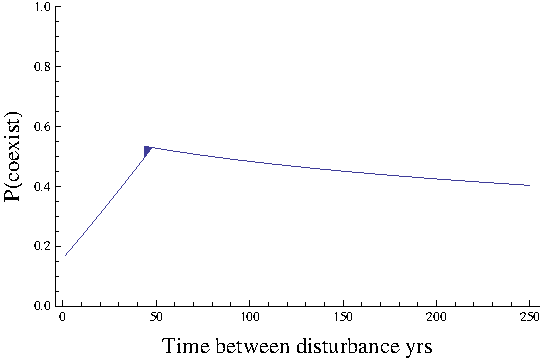
\includegraphics[width=2in]{fullintwTd.pdf}&&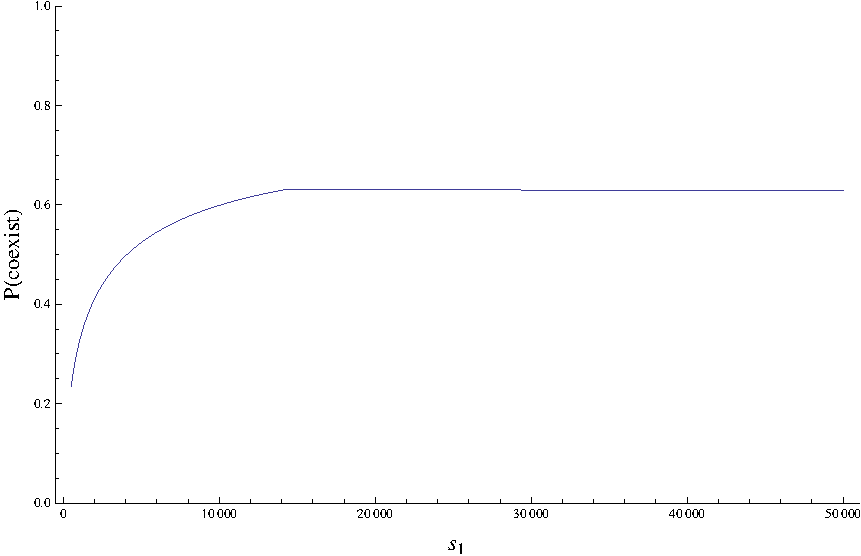
\includegraphics[width=2in]{fullintwiths1.pdf} \\
(e)&&(f)&\\
&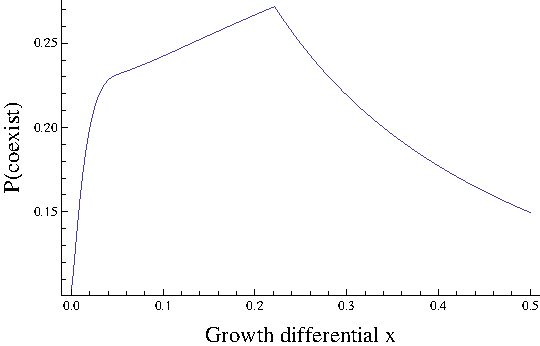
\includegraphics[width=2in]{fulltointwx.pdf}&&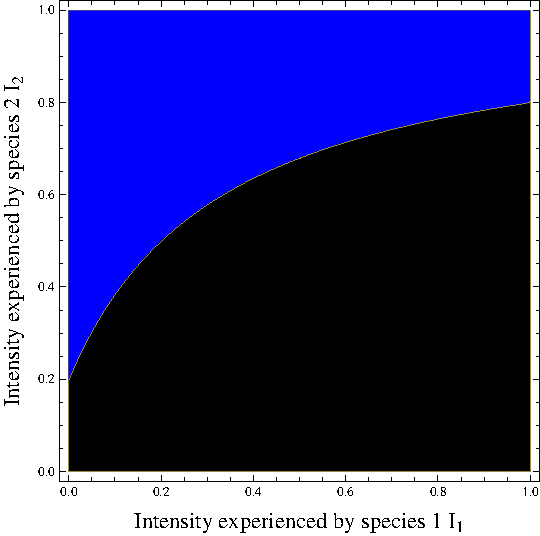
\includegraphics[width=2in]{fulllarges1.pdf}
\end{tabular}
\caption[Consequences of a three-dimensional trade-off]{\textbf{Three-dimensional trade-off:} (a) An example of $I-$space. The green/pale region to the bottom and right are where species 2 is dominant, while the blue/dark region (top and left) give species 1 monoculture. Where these regions overlap there is coexistence (black). (b),  (c) The change in the region of coexistence as $x$ varies, with a peak at intermediate values. (d) The size of the region given in (b) asymptotes as $s_1$ increases. Parameters $s_1=500,s_2=50,x=0.06,N=1000,T_D=10$ used to generate images unless specified. (e) The size of the region of coexistence and how it varies with $x$. The probability of coexistence increases rapidly with low $x$, and then experiences a slower increase for $0.046<x<0.22$. Above $x=0.22$ (f) When $s_1$ tends to infinity, a large proportion of $I-$space can support both species, although species 2 dominance is not possible ($s_1=10^6$).}
\label{full}
\end{figure}

\subsection{Linked intensities}
It is perhaps unrealistic to allow the responses to disturbance to  be unconstrained within $I-$space. Species specific responses are likely to be linked, such that as one increases, the other also increases. For example, a tropical storm may cause only low level disturbance intensities that differ between species. These species may still differ should the tropical storm develop into a hurricane. However, we would anticipate that this escalation of disturbance pressure would serve to increase the intensity experienced by both species. To simulate this, we consider the simplest, linear, case where $I_1=yI_2$, such that $y$ is a measure of the differences in the life history strategies of the two species, and $I_2$ is the force of a given disturbance event, normalised to the response of species 2. Note that for $y\neq 1$, one species will experience certain mortality while the other may retain some individuals. This occurs since when $I_2=1$, $I_1=y1=y\neq1$. Since $I_1$ is strictly increasing with $I_2$, when $0<y<1$ the intensity experienced by species one will be less than unity, $I_1<1$. Thus, while species 2 will go extinct in the next disturbance event, species 1 is expected to retain some of its population, and therefore colonise the entire community. Similarly, when $y>1$, when $I_2=1/y <1$, $I_1=1$ and species one will go extinct in the next disturbance, while species 2 can survive. As intensity increases beyond this point, the two intensities will converge at one, but as the species with the lower resistance already experiences extinction, this will not affect the likelihood of species coexisting.

In the three dimensional trade-off model, we consider the effects of changing $y$ on the range of disturbances that can give coexistence for the parameters $s_1=500,s_2=50,x=0.06,T_D=0.5$.

We can then plot the average change at the boundary as a function of $I_2$ for differing $y$. We find dramatically different behaviour as $y$ varies. For $y$ sufficiently large ($y>1.39$ for the current parameters), so that species 2 has a huge advantage in survival of a disturbance event, we find that for all intensities, coexistence does not occur, and species 2 exists in monoculture. Here, the increased fecundity of species 1 is not sufficient to overcome the dual advantage of species 2, with its superior juvenile growth rate and increased resistance to disturbance, as shown in Figure~\ref{linked}(a).

\begin{figure}[htbp]
\begin{tabular}{rrrr}
(a)&&(b)&\\
&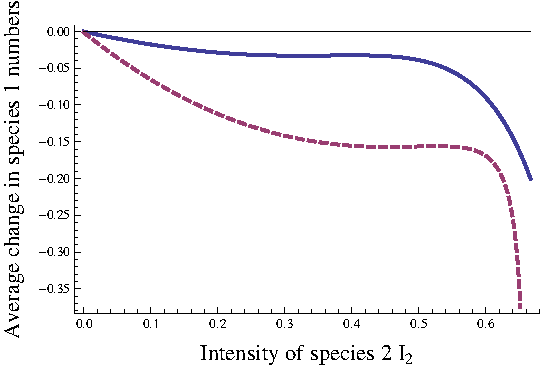
\includegraphics[width=2in]{highy.pdf}&&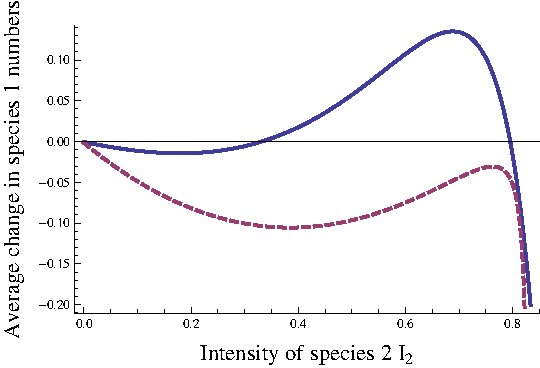
\includegraphics[width=2in]{lbworkubnot.pdf} \\
(c)&&(d)&\\
&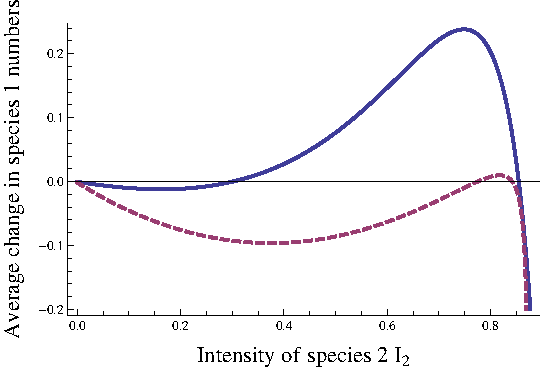
\includegraphics[width=2in]{fourbits.pdf}&&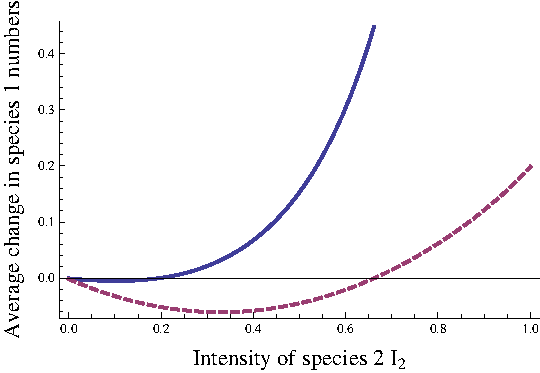
\includegraphics[width=2in]{onerooteach.pdf} \\
\end{tabular}
\caption[Effects of linking species specific disturbance intensities]{\textbf{Effects of linking species specific disturbance intensities:} Plots of $\text{AverageChange}(1)$ (solid) and $\text{AverageChange}(N-1)$ (dashed) for different $y$. Coexistence is expected to occur when the solid line is above zero, while the dashed line is negative. (a) $y=1.5$: $\text{AverageChange}(N-1)<1$ is satisfied for all intensities, but $\text{AverageChange}(1)>0$ never holds, so species 2 will exist in monoculture. (b) $y=1.2$:  $\text{AverageChange}(N-1)<1$ is satisfied for all intensities, but $\text{AverageChange}(1)>0$ holds for intermediate intensities. Therefore, coexistence will occur at intermediate intensities while at low and high intensities, species 2 will exist in monoculture. (c) $y=1.14$: Both curves have two real roots in the interval $[0,1]$, resulting in two bands of coexistence predicted by theory, with alternating monocultures surrounding them, species 2 monoculture at low and very high intensities, and species 1 at intermediate intensities. Note the higher band of predicted coexistence is not conformed by simulations, instead experiencing extinction of a random species due to the high intensity of disturbance events. (d) $y=0.9$: Both curves have a single real root in the interval $[0,1]$, resulting in a band of coexistence predicted by theory at intermediate intensity, with species 2 dominating at lower intensities while species 1 dominates at high intensities. $\text{AverageChange}(1)>\text{AverageChange}(N-1)$ for all $I_2$.}
\label{linked}
\end{figure}

As $y$ decreases, the behaviour then changes; $\text{AverageChange}(1)>0$ is satisfied for a range of intermediate disturbance intensities. At the same time, $\text{AverageChange}(N-1)$ remains below zero for all intensities $I_2$, meaning that coexistence is possible for intermediate intensities, but either side of this range species 2 will competitively exclude species 1 (Figure~\ref{linked}(b)). For the given parameters, the range of $y$ exhibiting this behaviour is approximately $1.16 \leq y \leq 1.38$. Decreasing $y$ further, making the two species response to disturbance more similar, the behaviour of the system changes once more. For $y\leq 1.15$, $\text{AverageChange}(N-1)$ has two real roots, and is positive between these roots. When $y>1$, both these roots occur in the interval $[0,1)$, as do two roots of $\text{AverageChange}(1)$. In this case, there are four distinct responses to disturbance as it increases in intensity (see Figure~\ref{linked}(c)). At low intensity, disturbance events are not strong enough to promote the more fecund species 1, so species 2 exists in monoculture. As intensity increases, then $\text{AverageChange}(1)>0$ is satisfied, while $\text{AverageChange}(N-1)<0$ continues to hold, giving coexistence of both species. Further increasing intensity, however, will result in $\text{AverageChange}(N-1)$ becoming positive. Here, species 2 will be competitively excluded, and species 1 will monopolise the system. Increasing intensity yet further results in $\text{AverageChange}(N-1)$ dropping back below zero, to give a secondary region where our invasion analysis predicts coexistence. However, for the parameters studied, the intensity here is high, and leaves a small remaining population (when $N=1000$, the remaining population is, on average, approximately 30 individuals). This reduced population is very susceptible to the stochasticity in the model, and all simulations result in one species going extinct by chance, although the identity of the surviving species varies between simulations. Increasing intensity even more, we have that $\text{AverageChange}(1)$ also drops below zero, so our theory predicts species two monoculture, which is once again matched by simulations, even given the extremely high intensities involved.

Once $y\leq 1$ there is only one root of $\text{AverageChange}(1)$ and one root of $\text{AverageChange}(N-1)$ in the interval $(0,1)$ (See Figure~\ref{linked}(d)). We therefore see a different type of behaviour again, with species 2 excluding the more fecund species 1 at low intensities, coexistence occurring at intermediate intensities, and species 1 excluding species 2 as high intensities.

As $y$ decreases towards zero, the range of intensities that can support both species will tend to a small interval, of width approximately $0.005$, at very low intensities ($0.005\lessapprox y \lessapprox 0.01$). We find that it is possible only to slightly increase the range of intensities giving coexistence from that of the case $y=1$, with $y=0.90$ (2 significant figures) giving a small increase in intensity range leading to coexistence. The probability of species with randomly selected, yet linked, intensities coexisting with $y=0.9$ is given by $0.4666$, only slightly larger than the probability of coexistence when $y=1$, given by $0.4663$, but this value declines again for $y<0.9$. That is, when the more fecund species 1 has a slight advantage in resistance to disturbance, the range of disturbances that the system can survive while maintaining its full biodiversity is maximised.

\section{Discussion}
Both life history trade-offs and disturbance events have been suggested as mechanisms that can promote and support high levels of diversity in nature \citep[e.g.][]{adler2000space,denslow1987tropical,sousa1984role,turnbull1999seed}. Here, we demonstrate that trade-offs among the three major life history traits for plants can give coexistence of at least two species competing within the same niche, and numerically quantify the likelihood of coexistence for each trade-off. However, the effectiveness of these trade-offs in supporting multiple species varies dramatically. Where species do not differ in juvenile growth rates, only small communities can possibly support more than a single species, and even in these small communities coexistence is extremely unlikely outside a very narrow range of parameters. This result suggests that a trade-off between seed production and resilience cannot realistically contribute to the diversity of a community. \textbf{This result has some support in the literature:} from the data in \cite{martin2010dispersal}, \cite{martin2010divergence} concluded that ``it is unlikely that... survivorship come[s] at the expense of fecundity.'' \textbf{However, some other studies do find a correlation between fecundity and defence \citep[e.g.][]{marquis1984leaf,gwynn2005resistance}. \cite{gwynn2005resistance} demonstrate that, at least for animals, parasite resistance comes with a reproductive cost, while \cite{muller2010tolerance} suggests there is a trade-off between fecundity and tolerance to shade or drought. However, \cite{muller2010tolerance} considers disturbance rate $m$ as a constant, identical across species, and as a separate parameter to species specific tolerance $h_i$, in a heterogeneous environment. Here, in contrast, we consider a homogeneous environment in which species react differently to pulses of increased death rate. While tolerance to constant environmental stress may indeed trade-off against fecundity, we propose that the limited evidence for a trade-off between survival of a pulse-type disturbance, such as a hurricane hitting a region of mature forest, and fecundity is a consequence of other, more strongly selected trade-offs such as the growth-survival and fecundity-growth trade-offs.}

Meanwhile, trade-offs between growth and either fecundity or disturbance resistance (or both) can support multiple species for any system capacity $N$. In a large system, we demonstrate that a trade-off involving all three of the major plant traits will give a probability of randomly selected disturbance resistances supporting two species higher than the probability given by a growth-defence trade-off alone. However, when species responses to disturbance are proportional (such that disturbance intensity for one species is doubled, the intensity for the second species is also doubled), the three dimensional trade-off does not significantly improve the likelihood of coexistence when compared to a fecundity-growth trade-off. These results suggest that the trade-off between fecundity and juvenile growth rate, or competition and colonisation, contributes much more to the maintenance of biodiversity than trade-offs involving disturbance resistance.  

The current model only includes two species, although disturbance is also anticipated to enhance coexistence in multi-species communities \citep[e.g.][]{loehle2000strategy,roxburgh2004intermediate}. Theory has shown that infinitely many species may coexist along a competition-colonisation trade-off \citep{tilman1994competition,adler2000space}, although this coexistence is either highly unlikely or structurally unstable \citep{nattrass2012quantifying, gyllenberg2005impossibility}. In Chapter~4, the current model is extended to three species for the trade-off between fecundity and growth, while the model where species differ in all three traits is also considered. For tradeoffs between defence and either fecundity or growth, we anticipate qualitatively similar results for a multi species model, whereby a fecundity-defence trade-off will be extremely sensitive to changes in parameters, while a growth-defence trade-off is expected to be ore robust. A further extension of the model is to include spatial structure. While Chapter~4 again considers this in a simplified manner, a full spatial structure may have dramatic effects on coexistence, due to the propensity for species to show within-species clustering \citep{condit2000spatial,murrell2001uniting} and limitations on dispersal. As in the fecundity-growth model discussed in Chapter~2, we anticipate that spatial structure may assist the weaker competitor, as restricted dispersal may allow it to win sites by default. \textbf{One further aspect that may influence the results is the fact many species in areas of high disturbance alter reproductive strategy. Foe example, many species subject to fire disturbance have a dormant seed bank \citep[e.g.][]{morgan1988seed,valbuena2001contribution}. This seed bank allows species to survive disturbances where all adult plants are destroyed. In the model considered here, the ability of adult individuals to withstand a disturbance makes them the equivalent of a dormant phase, yet the results may differ if dormancy occurs at the seed stage.}

We conclude that a trade-off between fecundity, in the form of per capita annual seed production, and juvenile growth rates is more significant in sustaining biodiversity than trade-offs between growth and defence or fecundity and defence, and while species specific reactions to disturbance can slightly improve the likelihood of a fecundity-growth trade-off allowing two species coexistence, this increase is not significant. This concurs with empirical studies, which have found a great deal of support for a trade-off between fecundity and growth rate, or the equivalent competition-colonisation trade-off \citep[e.g.][]{levins1971regional,yu2001competition,tilman1994competition,adler2000space}. The high level of occurrence for this trade-off indicates that it has been an important driver in the evolution of those diverse communities, allowing two or more species to effectively occupy the same resource niche by the different allocation of that resource to their life history traits. That a trade-off between growth and defence can support some coexistence suggests that some support should be found for this trade-off in empirical studies, and this is indeed the case \citep[e.g.][]{wright2010functional,fine2006growth}. However, support for this is much less widespread than the fecundity-growth or competition-colonisation trade-off, which further supports our conclusion that the latter is the more significant driver of biodiversity.

\section*{Appendices}

\bappendix
 \section{Approximating the expected change function}
 \label{appapproximations}
 The expected change for the model when at the lower boundary $n=1$ is given by
 \begin{align}
\label{acreal1difi}&\text{AverageChangeReal}(1)=\frac{-I_1+(N-1)I_2^{N-1}(1-I_1)}{dNT_D}\\
&+\frac{(1-I_1)\sum_{k=1}^{N-2}\sum_{j=k}^{N-2}k I_2^j(1-I_2)^{N-2-j}{N-2\choose j} Sp_1(1,N-1-j)^k(1-Sp_1(1,N-1-j))^{j-k} {j \choose k}}{dNT_D} \notag \\
 &+ \left(1-\frac{1}{dNT_D}\right)(P(\text{Increase}(1))-P(\text{Decrease}(1))), \notag
 \end{align}
 while at the upper boundary $n=N-1$, the expected change is given by
\begin{align}
 \label{acrealtotdifi}&\text{AverageChangeReal}(N-1)= \frac{-I_1^{N-1}(N-1) +I_2(1-I_1^{N-1})}{dNT_D} \\
 &-\frac{(1-I_2)\sum_{k=1}^{N-2}\sum_{j=k}^{N-2}k I_1^j(1-I_1)^{N-2-j}{N-2\choose j} Sp_1(N-1-j,1)^{j-k}(1-Sp_1(N-1-j,1))^{k} {j \choose k}}{dNT_D} \notag \\
 &+ \left(1-\frac{1}{dNT_D}\right)(P(\text{Increase}(N-1))-P(\text{Decrease}(N-1))). \notag
  \end{align} 
These are approximated using \eqref{ac}. Figure~\ref{fig:fdtoapprox} shows how the size of the absolute error between the actual expected change and the approximation declines with system capacity $N$ for a trade-off between fecundity and defence ($x=0$), while Figures~\ref{fig:growthdefenceerrors} and \ref{fig:fullapprox} show that this result holds for the growth-defence trade-off ($s_1=s_2$) and the three dimensional trade-off respectively. The error was calculated for intensities $I=0.1,0.2,0.3,...,0.9$ and time between disturbances $\ln(T_D)=1,2,3,...,8,$, therefore giving 648 error values for each system size. The approximation is accurate even at relatively small $N>400$. While the results from only one set of parameters are shown, these results are robust to parameter changes.

   
   
 \section{Roots of average change for $x>0$}
 \label{approots}
 Using Mathematica 8.0.1.0 to set $\text{AverageChange}(1)=0$ and rearranging to solve for $I_1$ gives the solution
 \begin{small}
 \begin{align}
 \label{lbr}
&\frac{-e^{-\frac{(I_2-1) s_2 (N-1) x}{N}} }{200 s_1 N (s_1+s_2 (N-2)) e^{\frac{s_2
   (N-2) x}{N}} \left(e^{-\frac{(I_2-1) s_2
   (N-1) x}{N}}-1\right)}\times \\
&\begin{pmatrix}
\begin{matrix}
s_1^2   \left(-100 N (I_2 (N-1)-1) e^{\frac{s_2 x   (I_2 (N-1)-1)}{N}} \right. \\
   \left. +((T_D-100) N-100)   e^{\frac{s_2 (N-2) x}{N}}-(N-1) (T_D   N-100)\right) \\
   +s_1 s_2 \left(\left(N^2 (100   (I_2-2)+T_D)-2 N (50 (I_2-2)+T_D)+200\right)\right. \\
  \left. e^{\frac{s_2 (N-2) x}{N}}-100 (N-2)   N (I_2 (N-1)-1) e^{\frac{s_2 x (I_2   (N-1)-1)}{N}}\right)\\
   +100 (I_2-1) s_2^2   (N-2) (N-1) N e^{\frac{s_2 (N-2)   x}{N}}
   \end{matrix} \\
\pm \sqrt{ \splitfrac{e^{-\frac{2 (I_2-1) s_2 (N-1)  x}{N}}}
{\splitfrac{ \left(s_1^2 \left(-100 N (I_2   (N-1)-1) e^{\frac{s_2 x (I_2   (N-1)-1)}{N}}+((T_D-100) N-100)   e^{\frac{s_2 (N-2) x}{N}}\right. \right. }
{\splitfrac{\left. -(N-1) (T_D N-100)\right)+s_1 s_2 \left(\left(N^2 (100   (I_2-2)+T_D)-2 N (50 (I_2-2)+T_D)+200\right) \right.}
{\splitfrac{   \left. e^{\frac{s_2 (N-2) x}{N}}-100 (N-2)   N (I_2 (N-1)-1) e^{\frac{s_2 x (I_2   (N-1)-1)}{N}}\right)}
{\splitfrac{\left. +100 (I_2-1) s_2^2   (N-2) (N-1) N e^{\frac{s_2 (N-2)   x}{N}}\right)^2}
{\splitfrac{-400 s_1 N (s_1+s_2   (N-2)) e^{\frac{s_2 x (I_2 (-N)+I_2+2   N-3)}{N}} \left(e^{-\frac{(I_2-1) s_2   (N-1) x}{N}}-1\right) \times}
{\splitfrac{ \left(100 I_2 s_1   (N-1) N (s_1+s_2 (N-2))   e^{\frac{s_2 x (I_2 (N-1)-1)}{N}}\right.}
{\splitfrac{\left.-(T_D   N-100) (s_2 (I_2   (-N)+I_2+N-1)+s_1)\right.}{\left. \left((s_1+s_2   (N-2)) e^{\frac{s_2 (N-2) x}{N}}+s_1   (-N)+s_1\right)\right)}}}}}}}}} 
\end{pmatrix} \notag
   \end{align}
   \end{small}
 Similarly, the solution for $I_1$ when $\text{AverageChange}(N-1)=0$ is given by
 \begin{small}
 \begin{align}
 \label{ubr}
&UBR(I_2)=-\frac{e^{\frac{(3-2 I_2) s_2 x}{N}}}{N 200 s_1 (N-1)^2 (s_1 (N-2)+s_2)
   e^{\frac{s_2 x}{N}} \left(e^{-\frac{(I_2-1) s_2
   x}{N}}-1\right)}\times \\
& \begin{pmatrix}\splitfrac{\pm T_D N
   e^{\frac{(2 I_2-3) s_2 x}{N}} \times}{
   \begin{matrix}  \sqrt{ \frac{  \splitfrac{(N-1)^2
   \left(e^{\frac{2 (3-2 I_2) s_2 x}{N}} \times \right.}{\splitfrac{\left(s_1^2
   (N-2) (N-1) (T_D N-100)
   e^{\frac{(I_2-2) s_2 x}{N}}\right.}{\splitfrac{-(s_1
   (N-2)+s_2) e^{\frac{(I_2-1) s_2 x}{N}}}{\splitfrac{
   \left(100 (I_2-1) s_2 N+s_1 \left(T_D
   (N-2) N-100 \left(N^2-2\right)\right)\right)}{\splitfrac{\left. +100
   s_1 N (I_2-N+1) (s_1
   (N-2)+s_2) e^{\frac{2 (I_2-1) s_2
   x}{N}}\right)^2}{\splitfrac{-400 s_1 N (s_1
   (N-2)+s_2) e^{-\frac{2 (I_2-2) s_2 x}{N}} \times }
{\splitfrac{ \left(e^{-\frac{(I_2-1) s_2 x}{N}}-1\right)\times}{\splitfrac{ \left(s_1
   (N-2) (N-1) (T_D N-100) (-I_2
   s_2+s_1 (N-1)+s_2) e^{\frac{(I_2-2) s_2
   x}{N}}\right.}{\splitfrac{+(N-2) (T_D N-100) (s_1
   (N-2)+s_2) ((I_2-1) s_2+s_1
   (-N)+s_1) e^{\frac{(I_2-1) s_2 x}{N}}}{\left. \left.+100
   I_2 s_1 (N-1) N (s_1
   (N-2)+s_2) e^{\frac{2 (I_2-1) s_2
   x}{N}}\right)\right)}}}}}}}}}}
   {T_D^2 N^2}} \\
         +s_1^2   (N-2) (N-1)^2 (T_D N-100)   \left(-e^{\frac{(I_2-2) s_2 x}{N}}\right) \\
   +(N-1)   (s_1 (N-2)+s_2) \left(\left(100 (I_2-1) s_2   N\right. \right. \\
   \left.+s_1 \left((T_D-100) N^2-2 T_D   N+200\right)\right) \times \\
    \sinh \left(\frac{(I_2-1) s_2   x}{N}\right)\\
   +\left(100 (I_2-1) s_2 N+s_1   \left((T_D-100) N^2-2 T_D N+200\right)\right) \\
   \cosh \left(\frac{(I_2-1) s_2 x}{N}\right)+100 s_1   N (-I_2+N-1) \sinh \left(\frac{2 (I_2-1) s_2   x}{N}\right) \\
  \left.+100 s_1 N (-I_2+N-1) \cosh   \left(\frac{2 (I_2-1) s_2  x}{N}\right)\right)
   \end{matrix}} \end{pmatrix} \notag
  \end{align}

  \end{small}
 Note that for both the growth-defence trade-off, and the full three dimensional trade-off that also includes fecundity, one of the roots here is always above one. These roots are the positive square root for $LBR(I_2)$, and the negative root for $UBR(I_2)$. Therefore, the roots used to calculate the size of the region of coexistence are the negative and positive roots respectively.

 
   \begin{figure}[th]
\centering
   \begin{tabular}{rrrr}
   (a)&&(b)&\\
  &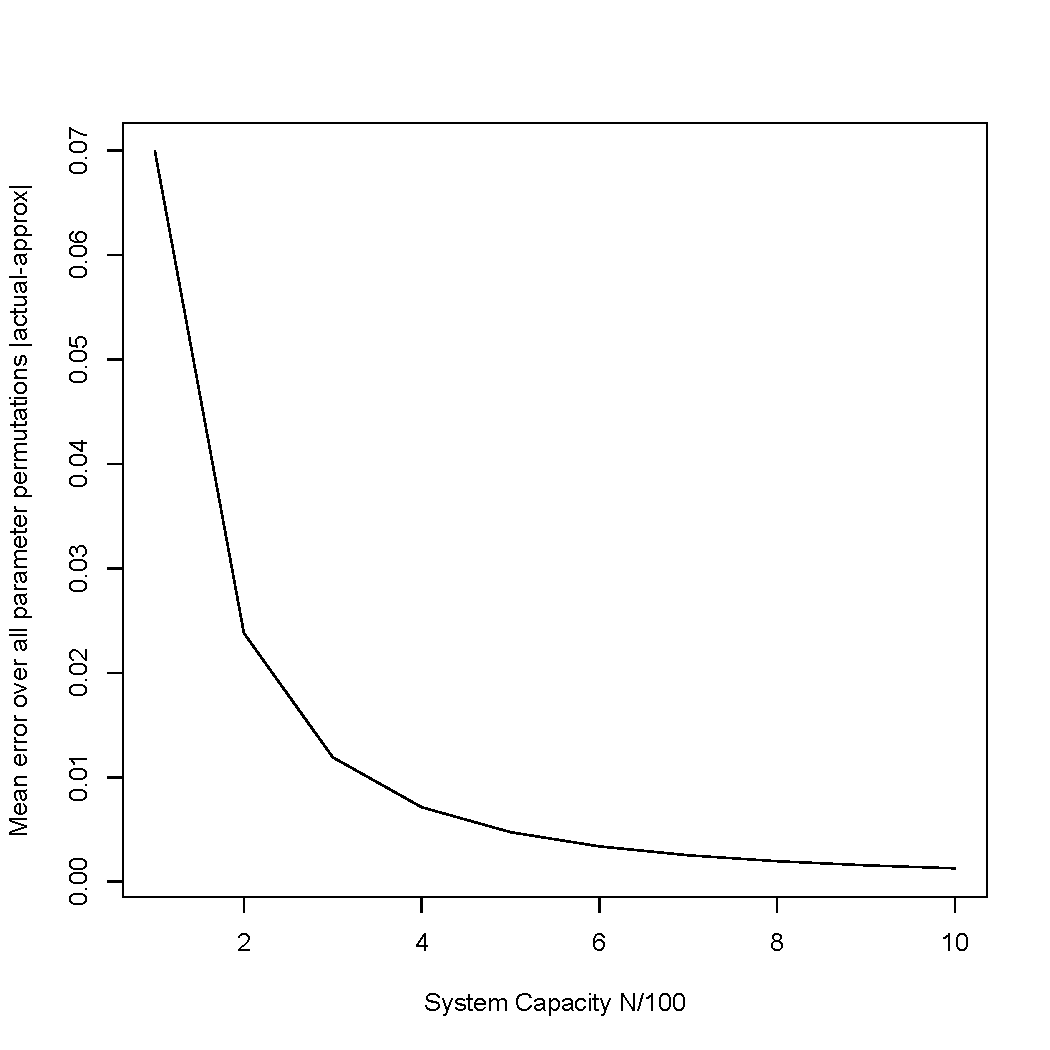
\includegraphics[width=2.5in]{FDmeanerr.pdf} && \includegraphics[width=2.5in]{FDmaxerr.pdf} \\
  (c)&&(d)&\\
  &\includegraphics[width=2.5in]{FDtmeanerr.pdf} && \includegraphics[width=2.5in]{FDtmaxerr.pdf} \end{tabular}
   \caption[Errors in approximating average change: fecundity-defence trade-off]{\textbf{Fecundity-defence trade-off:} (a-b)  How the mean (a) and maximum (b) error size at the lower boundary decrease with increased system capacity $N$. (c-d) How the mean (c) and maximum (d) error size at the upper boundary decrease with increased system capacity $N$. The error was calculated for intensities $I_1,I_2=0.1,0.2,0.3,...,0.9$ and time between disturbances $\ln(T_D)=1,2,3,...,8.$ Parameters used are $s_1=500,s_2=50$. Error is calculated as $| \text{AverageChangeReal}(n) - \text{AverageChange}(n) |$ for $n=1,N-1$.}
    \label{fig:fdtoapprox}
   \end{figure}
   
    \begin{figure}[th]
\centering
   \begin{tabular}{rrrr}
   (a)&&(b)&\\
  &\includegraphics[width=2.5in]{GDmeanerr.pdf} && \includegraphics[width=2.5in]{GDmaxerr.pdf} \\
  (c)&&(d)&\\
  &\includegraphics[width=2.5in]{GDtmeanerr.pdf} && \includegraphics[width=2.5in]{GDtmaxerr.pdf} \end{tabular}
   \caption[Errors in approximating average change: growth-defence trade-off]{\textbf{Growth-defence trade-off:} (a-b)  How the mean (a) and maximum (b)  error size at the lower boundary decrease with increased system capacity $N$. (c-d) How the mean (c) and maximum (d) error size at the upper boundary decrease with increased system capacity $N$. The error was calculated for intensities $I_1,I_2=0.1,0.2,0.3,...,0.9$ and time between disturbances $\ln(T_D)=1,2,3,...,8.$ Parameters used are $s_1=50,s_2=50,x=0.06$. Error is calculated as $| \text{AverageChangeReal}(n) - \text{AverageChange}(n) |$ for $n=1,N-1$.}
     \label{fig:growthdefenceerrors}
    \end{figure}
    
     \begin{figure}[th]
\centering
   \begin{tabular}{rrrr}
   (a)&&(b)&\\
  &\includegraphics[width=2.5in]{FDGmearerr.pdf} && \includegraphics[width=2.5in]{FDGmaxerr.pdf} \\
  (c)&&(d)&\\
  &\includegraphics[width=2.5in]{FDGtmearerr.pdf} && \includegraphics[width=2.5in]{FDGtmaxerr.pdf} \end{tabular}
   \caption[Errors in approximating average change: three dimensional trade-off]{\textbf{Fecundity-growth-defence trade-off:} (a-b)  How the mean (a) and maximum (b) error size at the lower boundary decrease with increased system capacity $N$. (c-d) How the mean (c) and maximum (d) error size at the upper boundary decrease with increased system capacity $N$. The error was calculated for intensities $I_1,I_2=0.1,0.2,0.3,...,0.9$ and time between disturbances $\ln(T_D)=1,2,3,...,8.$ Parameters used are $s_1=500,s_2=50,x=0.06$. Error is calculated as $| \text{AverageChangeReal}(n) - \text{AverageChange}(n) |$ for $n=1,N-1$.}
     \label{fig:fullapprox}
   \end{figure}
   
   \eappendix
   


\newpage
\chapter{Multi-species coexistence: the effects of disturbance refugia on species richness}
\newpage
\topskip0pt
\vspace*{\fill}
\section*{Abstract}
Determining the size and structure of nature reserves that are best suited to preserving biodiversity and abundance is an important question for conservation, although it has received little theoretical attention. We examine the effects of introducing protected reserves where disturbance pressure is removed, and investigate the effects of varying the size of these reserves, by expanding the model presented in Chapter~2 to include both additional species and a metapopulation structure. We find that spatial heterogeneity in disturbance pressure is necessary to support $n>2$ species in a community, while protected reserves are most likely to increase $\gamma$ diversity when they are smaller. We observe no relationship between reserve size and within-reserve $\alpha$ diversity, although when reserves are small, an increase in species richness in the neighbouring, unprotected area is observed.
\vspace*{\fill}
\newpage
\section{Introduction}
Studies have suggested that disturbance, caused by either natural or human events, play an important role in maintaining high levels of species richness in a community \cite{connell1978diversity,huston1979general,sousa1984role,schoener1974resource}. Most commonly, the case where the ability to colonise an empty habitat is traded off against local competitiveness is considered \citep[e.g.][]{tilman1994competition, cadotte2006testing}. In a constant environment, the poorer local competitor will be excluded, yet disturbance events can enable the persistence of this poor competitor in the community by creating empty habitat. Then, the greater colonising ability of the poor competitor enables long term survival \citep{sousa1984role,denslow1987tropical,connell1978diversity,grime1973competitive,huston1979general}. It has been argued that there are at least three main axes upon which disturbance should be measured \cite{malanson1984intensity,miller1982community,sousa1984role}, yet few theoretical studies have considered the interaction of these factors; frequency; intensity; extent. Here, frequency is measured by the expected time between disturbances, intensity the mean proportion of the exposed community killed during a disturbance, while extent is a measure of the proportion of a community exposed to a disturbance event. For example, a treefall event within a forest is expected to be highly frequent, yet with very low intensity and extent, as very little of the community is affected. On the other hand, forest fires are likely to be less frequent, while covering a varying proportion of the community (extent). Individuals within the exposed area are likely to experience high mortality, therefore fire disturbances are expected to have high intensity. Chapter 2 shows an analysis of how the effects of frequency and intensity of disturbance differ, as do \cite{miller2011frequency}, but consideration of extent has been limited in theoretical models.

Within community ecology, different processes act at different spatial scales \citep{levin1992problem}. In particular, the effects of disturbance may appear spatially uniform at a local scale, while at a regional level there is observed spatial structure. This spatial structure may cause different regional diversity patterns than predicted by randomly distributed disturbances \cite{vuilleumier2007patch}. Regional processes affect local outcomes \cite{holt1993ecology}. This multi-scale structure is often modelled using a metapopulation structure, where regional processes act on patches that experience their own local population dynamics. These patches can be interpreted as whole communities, or a site occupied by a single individual \cite{tilman1994competition,calcagno2006coexistence}.

Theory has shown that in a metapopulation system under disturbance, transitive competition networks have lower diversity than intransitive networks \citep{caswell1991disturbance}. Further, when patch quality varies, source sink dynamics can occur, where by a species is prevented from going extinct in one patch (the `sink') by immigration from a patch where it experiences conditions whereby it can persist (the `source')  \citep{pulliam1988sources}. Theory suggests optimal management for preserving communities is to focus attention on source patches \citep[e.g.][]{runge2006role}, although determining best practice can be complex even when disturbance affects every patch equally \citep{strasser2012contributions}.

Some management strategies such as nature reserves or no take zones in fishing territories can provide a mechanism by which disturbance is not uniform on a regional scale. However, there is disagreement on whether a single large reserve or several small reserves most efficiently protect diversity \citep{simberloff1982refuge}. \cite{simberloff1991nestedness} argued that small reserves may increse reginal $\gamma$ diversity when competitive exclusion is important, via reduced dispersal of dominant species, while \cite{ovaskainen2002long} suggest that time to extinction is maximised for intermediate reserve size. Recent work by \cite{lasky2013reserve} indicates that reserve size selection may consist of a trade-off between $\alpha$ and $\gamma$ diversity, where the former is maximised for large reserves containing many species, while smaller reserves may contain less species locally, yet maximise the species richness at the landscape scale ($\gamma$ diversity). However, the reserve size question has received little attention from a spatial community theory perspective.

Here, we use a nested patch model to examine the effects of disturbance extent on species richness. On a local scale, patches represent a single individual, while regionally, each of two patches represents a community of individuals. We demonstrate that only two species can coexist along a fecundity-growth trade-off when only a single scale is considered, yet when both regional and local dynamics are accounted for, three species can coexist, demonstrating that nature reserves can increase $\gamma$, or regional, diversity. Moreover, we show that this coexistence can occur at a local level (increased $\alpha$ diversity) when limited seed exchange between the regional patches occurs, and that this increase in local diversity may be observed in the regions neighbouring a reserve, rather than within the reserve itself. The potential management consequences of these results in the case where disturbance is human induced (for example forestry) are discussed.



\section{The Model}
Here we extend the lottery-type trade-off model (of Chapters 2 and 3) to include a third species, to determine whether a simple trade-off can support many species. The model assumes a completely filled canopy, from which there is then a death of an individual chosen at random. If the population of species $i$ is given by $n_i$, then species $i$ will be the identity of the randomly selected individual with probability
\begin{equation}
\label{d}
d_i(n_1,n_2,n_3)=\frac{n_i}{n_1+n_2+n_3}=\frac{n_i}{N} \end{equation}
for $i \in \{1,2,3\}$. Once this death has occurred, the remaining individuals in the system compete over the gap that has appeared. If the species differ in juvenile growth rates $g_i$, then if two species are competing over a site, it is simple to show that the slower growing species $i$ must be present in the site alone for time $x_{i,j}=C(1/g_i +1/g_j)/2$, where $C$ is the size of an adult individual, otherwise the rapidly growing species $j$ will outcompete it

\textbf{We assume that species 1 is the most fecund, while species 3 is the species that grows most rapidly. Species 2 is considered to be a generalist, with intermediate seed production and juvenile growth rate. That is;
\begin{align}
s_1&>s_2>s_3,\\
g_1&<g_2<g_3.
\end{align}
We note that species 1 will colonise a gap if it arrives first, and is not invaded by either species 2 or 3. Therefore, assuming that seeds are dispersed via a Poisson process (with rate $\lambda_i=s_iN_i(t)/N$), the probability of species 1 colonising a gap is given by
\begin{equation}
\label{c1}
c_1(n_1,n_2,n_3)=\frac{s_1 n_1 \exp(-s_2x_{1,2}n_2/N)\exp(-s_3x_{1,3}n_3/N)}{\sum_{k=1}^3 s_k n_k},\end{equation}
where $s_i$ is the annual seed production per capita for species $i$.}

There are two possible ways in which species 2 can claim a gap. First, if species 2 arrives in the gap first, and species 3 fails to invade in time $x_{2,3}=x_{1,3}-x_{1,2}$, or second, if species 1 colonises the site first, yet is invaded by species 2 within time $x_{1,2}$, while species 3 does not invade this secondary invasion. The first case occurs with probability
$$
\frac{s_2 n_2\exp(-s_3x_{2,3}n_3/N)}{\sum_{k=1}^3 s_k n_k},
$$
but the second case is slightly more complex.species 1 colonises the site first with probability $s_1n_1/(\sum s_kn_k)$. This is then invaded by an undetermined individual with probability $1-\exp(-s_2x_{1,2}n_2/N)\exp(-s_3x_{1,3}n_3/N)$, and the identity of this successful invader is species 2 with probability $s_2/(s_2+s_3)$. Finally, species 3 cannot invade this species 2 juvenile (probability $\exp(-s_3x_{1,3}n_3/N)$). Note that if $s_3=0$, the ratio $s_2/(s_2+s_3)=1$ for all $s_2 \neq 0$, and that if $s_2=0$, then the ratio is simply $0$ for $s_3 \neq0$, meaning that since one species must go extinct before the other (in the non disturbance case), the singularity at $s_2+s_3=0$ can be approximated by the appropriate limit ($1$ or $0$ depending on the identity of the species to go extinct first). Thus, the probability of species 2 claiming an empty site is given by
\begin{align}
\label{c2}
c_2(n_1,n_2,n_3)=&\frac{s_1 n_1(1-\exp(-s_2x_{1,2}n_2/N)\exp(-s_3x_{1,3}n_3/N))}{\sum_{k=1}^3 s_k n_k}\frac{s_2 n_2\exp(-s_3x_{2,3}n_3/N)}{s_2n_2+s_3n_3} \notag \\
&+\frac{s_2 n_2\exp(-s_3x_{2,3}n_3/N)}{\sum_{k=1}^3 s_k n_k}
\end{align}
Species 3 will invade any site that the others fail to claim. If species 3 arrives first, invades the first coloniser quickly, or invades a specie 2 juvenile that has displaces a species 1 individual, then the gap will go to species 3. It is simple to show that these all add to one, so for simplicity of notation, we define the probability of species 3 colonising as
\begin{equation}
\label{c3}
c_3(n_1,n_2,n_3)=1-c_1(n_1,n_2,n_3)-c_2(n_1,n_2,n_3).\end{equation}

\subsection{Disturbance events}
Disturbance events in the model are events that kill a proportion of individuals within a single time step, opening up an increased number of gaps for the individuals to compete over, favouring $r-$strategists. We model these events that occur within an event step with probability $f=(dT_DN)^{-1}$, where $d=0.01$ is the intrinsic annual death rate, and $T_D$ is the expected number of time steps between disturbances. Within a disturbance event, each individual of species $i$ will be killed with a probability $I_i$, which therefore represents both the probability of an individual dying, and the expected mortality rates for species $i$ during the disturbance. Once all $D$ deaths have occurred (each individual has been subjected to mortality of rate $I_i$), the remaining adults will compete over the resulting gaps in the forest canopy. Each gap is `assigned' a new adult using the formulae given by \eqref{c1}, \eqref{c2} and \eqref{c3}. However, note that in a disturbance event, it is possible that 2 or more species go extinct simultaneously. If only two species survive the disturbance event, the probabilities for recolonisation in Chapter 2 are used, while if only one species survives, it will claim all sites. In the rare event where all individuals are destroyed in a disturbance, the system is considered extinct. 

The effects of dispersal limitation and localised disturbance on the results are also examined while treating spatial patterns implicitly. The system capacity $N$ is divided into two smaller regions $N_1,N_2$ which each experience different disturbance regimes. For example, the region $N_1$ may be protected from disturbance by some geographical feature, which may also limit the connectedness of the two regions. Dispersal limitation is considered by reducing the level of colonisation between these two regions, such that a proportion $\alpha_{i,j}$ of seeds will transfer from region $i$ to region $j$. Populations of species $k$ in region $i$ are denoted $n_{i,k}$ in this section of the results. Note that when considering colonisation in region $i$, average seed numbers of species $k$ are given by $(1-\alpha_{i,j})n_{i,k} + \alpha_{j,i}n_{j,k}$, where $j$ represents the other region, rather than $s_k n_{i,k}$ as previously. 

\section{Results}
\subsection{Homogeneous environment}
We examine the persistence of the three species over a range of $x-$space. Since $x_{2,3}=x_{1,3}-x_{1,2}$, we can consider different combinations of 
$x_{1,2}$ and $x_{1,3}$ to get a complete picture of the parameter space for growth rates for the species. Using fixed seed numbers $s_1=500,s_2=100,s_3=20$ we can examine the bahaviour of the system under many different circumstances by simply varying the $x_{i,j}$s (See Figure~\ref{xregions}). We simulate populations of several different combinations of $x_{1,2}$ and $x_{1,3}$ and examine the effects of =moving between regions of $x-$space shown in Figure\ref{xregions}, while also examining the effects of the initial populations on the outcome. We run simulations varying initial populations by 100 each time, considering all combinations of $n_1,n_2,n_3$ that (a) Satisfy that each species begins with $100q$ individuals present for $q \in \{1,2,3,4,5,6,7,8\}$ and (b) the three populations add to $N=1000$. 
\begin{figure}[htbp]
\begin{center}
\includegraphics[width=4in]{3dxchoices.pdf}
\caption[The different regions of $x-$space]{\textbf{The different regions of $x-$space:} The regions of $x-$space that give coexistence for the 3 possible species pairs. Species 1 and 2 can coexist between the red lines. Species 1 and 3 coexist between the black lines, while species 2 and 3 can coexist between the blue lines.}
\label{xregions}
\end{center}
\end{figure}
When species 3 dominates both species 1 and 2 (top left), it dominates the three species environment as expected, driving both other species to extinction. Similarly, when species 1 excludes each of the two less fecund species, it also dominates the three species case. However, when species 2 dominates both the more fecund species 1 and the faster growing species 3 in pairwise competition, in the right hand side region of Figure\ref{xregions}, where this occurs, there is an element of founder control. When species 3 excludes species 1 in pairwise competition, the outcome is driven by the initial populations, if species 2 is initially at a much lower population than species 3, species 3 will persist in monoculture, while if the initial population of species 2 is sufficiently high, it will exclude both the fecund species 1 and the fast growing species 3. Similarly, when species 1 excludes species 3, if the species 2 population in initially low, then species 1 will dominate the environment, while for higher initial populations species 2 dominates. When species 1 and 3 can coexist but are both excluded by species 2, in the three species case, it is necessary for species 2 to have a high initial population in order to persist, in which case it will exclude both other species. However, if it has a lower initial population, then it will be excluded and species 1 and species 3 will coexist together.

A similar pattern is observed when species 2 can coexist alongside one of the other species, yet excludes the third species. When species 2 and 3 can persist together, and species 2 excludes species 1, then founder control again occurs. If $n_2(0)$ is sufficiently high, species 1 will be driven to extinction and the species 2 and 3 coalition will persist, but if the initial population is too low, species 2 will be excluded, and the outcome of the model simulations is determined by the two species interactions between the fecund species 1 and the rapidly growing species 3. Similarly, when species 1 and 2 can coexist, and species 2 excludes species 3, a sufficiently low initial population will instead result in species 2 being excluded, and the outcome is determined by the interactions of species 1 and 3, while a high initial population will exclude species 3, allowing the species 1 and 2 coalition to thrive.

In all other cases, species 2 is excluded regardless of initial populations, and the behaviour of the model is determined by the two species analysis of species 1 and 3.

\subsection{Disturbance with equal effects on all species} \label{ss:homo}
When setting $I_i=I$ for all $i \in \{1,2,3\}$, such that disturbance effects all species equally, the response of the system to disturbance is determined by the non disturbance behaviour. We assume frequency is sufficiently high to not have a significant effect (see Chapter 2) and consider the impact of increasing disturbance intensity. If species 1 excludes both other species in a homogeneous environment, the only effect disturbance has is to accelerate this. When species 1 coexists with either species 2 or species 3 in the homogeneous environment, then as disturbance intensity increases, it will exclude the $K-$ competing species, although they will still coexist at low intensity. When either species 2 or species 3 exists in monoculture in a disturbance free environment, as intensity is increased they will coexist along side species 1. When intensity is increased further, species 1 will exclude the $K-$strategists. When species 2 and 3 coexist in the disturbance free case, intensity can cause different community structures. At low intensity, species 2 and 3 will continue to exclude species 1. As intensity increases, the generalist species 2 will exclude both the $K-$strategist species 3 and the $r-$strategist species 1. Increase intensity further, and species 1 and 2 will coexist while species 3 is excluded, while at very high intensities, species 1 will exclude both species 2 and 3.

\subsection{Adding a defence specialist}
In most cases, the generalist species 2 is outcompeted by the two specialists eroding some of its niche from either side. Does a specialisation in defence against disturbance allow species 2 to sustain itself alongside the growth and colonisation specialists? We set $I_1=I_3=yI_2$, and vary $y>1$ so examine the effects of defence specialism by species 2. We find that increasing the disturbance intensity will initially just repeat the anticipated behaviour when all 3 species suffer the same intensity.. For $y$ sufficiently close to 1 ($y=1.1$), this will continue and the `expected' behaviour will occur. However, for larger $y$ ($y=2,10$), as intensity is increased further, the advantage in disturbance survival for species 2 becomes the dominant force behind the dynamics, and both species 1 and 3 are excluded, with species 2 existing in monoculture. We conclude that resistance to disturbance mortality of the generalist cannot increase biodiversity along a fecundity-growth trade-off.

\subsection{Patchy disturbances; regions of the forest protected from disturbance}
When disturbance regimes do not differ, but one of the three species is absent initially from region $i$, allowing the region wide persistence of all three species, any $\alpha_{i,j},\alpha_{j,i}>0$ will result in region wide exclusion of one of the three species. We therefore focus on a region of trait space whereby any of the three species can persist at differing levels of intensity for high frequency disturbances. From \ref{ss:homo} we thus choose a region of $x-$space whereby the result in a homogeneous environment is that the strong local competitor species 3 and the generalist species 2 coexist, while excluding the fecund species 1. One such choice of parameters is given in Table~\ref{tab:paras}, which we use henceforth. Note that for these chosen parameters, species 2 will be excluded in the non disturbance case when it's initial population is too low. We select initial populations whereby species 2 has a sufficiently high population to persist in the environment ($n_{i,2}(0)=0.5N_i,n_{i,1}(0)=0.3N_i$). Then species 1 is present when disturbance frequency is high and for intensities $I\geq0.75$, which species 3 persists in the system for low intensities $I\leq 0.15$. Meanwhile, species 2 will persist for all intensities $I\leq 0.8$.
\begin{table}[htdp]
\begin{center}
\begin{tabular}{|c|c|} \hline
Parameter & Value\\ \hline
$s_1$&500\\
$s_2$&100\\
$s_3$&20\\
$x_{1,2}$&0.05\\
$x_{1,3}$&0.1\\
$N$&2000\\ \hline
\end{tabular}
\end{center}
\caption{Parameters used for examination of patchy disturbance}
\label{tab:paras}
\end{table}
We assume that Region 1 (size $N_1$) does not experience any disturbance (although simulations give qualitatively similar results providing the disturbance regime in this region is of sufficiently low intensity to allow the persistence of the least fecund species). For example, this may be a nature reserve where logging is prohibited, while the second region experiences disturbance via logging. Thus, when entirely unconnected to the second region, species 2 and 3 will persist. We then study the effects of varied intensities (homogeneous across all species) of disturbance in the second region for a fixed frequency ($T_D=5$), which also examining the impact of differing the size of the disturbed region in a total forest of fixed size $N=2000$, and the level of reproductive connectedness between the two patches. Note that $\alpha_{i,j}=N_j/N$ represents perfect mixing of the two populations, with entirely random seed allocation. Only disturbance intensities above $I_{2,k}=0.75$ (for $k=1,2,3$) are considered, to ensure that all three species are present when the regions are unconnected.

As connectedness of the two regions ($\alpha_{i,j}, i,j=1,2$) is increased, with seed dispersal or alternative processes such as human induced migration linking the two sites, it becomes possible for the regional processes allowing multi-species coexistence to inflate local biodiversity. As shown in Figure~\ref{fig:regions}, the migration of seeds creates coexistence of three species in the disturbed region 2, as the refuge region has much fewer gaps created. This makes it more difficult for the excluded, fecund, species to invade. In the disturbed region, however, there are a larger number of gaps are created when a disturbance occurs, thus increasing the probability of settlement by the poor coloniser (species 3), which would be excluded should there be no immigration from the refuge.

\begin{figure}[htbp]
\begin{center}
\includegraphics[width=4.5in]{RegionsPlot.pdf}
\caption[Simulations with limited between-patch dispersal]{Restricted migration between a region without disturbance (region 1) and a region with high frequency, high intensity disturbances (region 2) can allow for three species coexistence at the local level. The disturbed region outside the refuge displays increased diversity when compared with regions that are not connected by seed dispersal, in which case the least fecund species would be excluded. Note that species richness within the refuge is not increased, despite the positive effect on regional richness.}
\label{fig:regions}
\end{center}
\end{figure}


\subsubsection{Effects of varied refuge patch size}
As the proportion of the forest protected from disturbance $N_1/N$ is varied, we find that the range of connectedness ($\alpha_{1,2}=\alpha_{2,1}=\alpha$, which is varied in increments of 0.05) for which all three species can persist at a given intensity is maximised at an intermediate value of $N_1/N$, as shown in Figure~\ref{fig:alpharange}. Only refuges below a certain proportion of the community can support all three species when there is mixing between the two regions. When the refuge becomes large, and the unprotected area small, the effect is to reduce the population of the fecund species 1. As this species requires the space creates by disturbance events to survive in the environment, the limited amount of space created by a disturbance, combined with the high mortality of species one in this part of the environment, results in the extinction of the most fecund species.

\begin{figure}[ht]
\label{fig:alpharange}
\includegraphics[width=4.5in]{refugesize.pdf}
\caption[Effects of refuge size on multi-species coexistence]{The effects of varied refuge size of the likelihood of three species coexistence. Shaded areas represent the coexistence of all three species regionally after 50000 event time-steps. When $\alpha>0$, coexistence is only possible for relatively small refuges, while when the protected region is significantly larger than the disturbed area, coexistence is not possible for any non-zero level of cross-colonisation.}
\end{figure}

\section{Discussion}
Understanding the ways in species diversity is generated and supported is a crucial problem in ecology, with great relevance for conservation practices. The role of environmental variability, such as disturbance events, is an important area of consideration. This is becoming more crucial, as climate change is predicted to have dramatic impacts on the frequency and intensity of such events \citep[e.g.][]{webster2005changes}. Here, the possibility of multi-species ($n>2$) coexistence is examined in an environment defined by the disturbance regimes. Within this model framework, with species differing only along a fecundity-growth trade-off, it is only possible for more than two species to coexist if the environment has some spatial heterogeneity combined with the temporal heterogeneity of disturbance events. In this case, the existence of a protected region that does not experience disturbances that effect the neighbouring region (for example, a nature reserve where logging is prohibited, or a no-take zone alongside a heavily trawled region of ocean) can promote region wide coexistence of greater than two species. In addition, if limited dispersal occurs between the two regions, it is possible that the local species richness outside the protected region will also be increased, without observing a corresponding increase within the reserve. This may have important consequences for the placement and management of nature reserves, which often seek to cover environmental regions that support all species \citep[e.g.][]{margules1988selecting,scott2001nature}.

The coexistence of three species within this model framework appears to be more robust when the protected area, or refuge, is relatively small in comparison with the neighbouring environment. Small protected areas in large areas experiencing disturbance can enable the region-wide support of multiple species for much higher levels of dispersal between the disturbed and protected regions. \textbf{This concurs with the findings of \cite{lasky2013reserve}, who find $\gamma$ diversity is maximised for small reserves. This indicates that under some circumstances, where disturbance comes in the form of human pressure such as logging, it may be possible that careful management of the system would allow for a large area to be logged, while the region continues to support a large number of species.
\cite{lasky2013reserve} find that large reserves have higher $\alpha$ diversity, we find that there is no relationship between the number of species present within the reserve. Instead, the boost in $\gamma$ diversity gained by small reserves is triggered by an increase in an increase in species richness in the unprotected region neighbouring the reserve.}

However, it is only possible for two species to coexist when the environment is considered as a single patch, with no spatial heterogeneity, either with or without disturbance events. This result in the non-disturbance case, where the environment is both spatially and temporally homogeneous, lends support to previous predictions that coexistence is unlikely when species face a trade-off affecting per capita reproduction, such as the fecundity-growth trade-off considered here \cite{egas2004evolution}.
 However, these results appear to conflict with empirical data, where coexistence of generalists and specialists is common \citep[e.g.][]{morris1996coexistence,bonesi2004differential}. 
 
 Further, if all three species are present in a single, isolated patch at $t=0$, then the generalist species (here species 2) can only persist in the environment when the initial population is sufficiently high, in both environments with and without disturbance. This result is in contrast to those of both \cite{marvier2004habitat} and \cite{nagelkerke2013coexistence}, who find short term disturbances tend to favour generalist species. This difference may be caused by the assumption by Marvier et al. that species that spread tend to be generalists, while the model presented here assumes that the more fecund species is the most successful coloniser, and therefore is the species to benefit from the creation of a large number of empty sites. A second assumption here is that all species can survive in isolation across the entire disturbance gradient (providing $I_i<1$), and the niche segregation into fecundity specialist and light competition specialist is dependent on the specific species composition of the region. In contrast, both the model of Marvier et al. and that of Nagelkerke and Menken assume specialist species can only survive in certain habitat types, independent of the presence or absence of a competing species. The current model also predicts that allowing the generalist species an advantage in disturbance defence does not permit multi-species coexistence. This may be because an increase in fecundity and an increase in defence against disturbance effectively operate along the same environmental axis, both increasing fitness within a disturbance event.
 
 The results presented here emphasise that disturbance can be a key contributor to species richness, and that considering different factors that make up disturbance can be crucial in predicting how a community will respond to disturbance pressure (see also Chapter~2). Here, the effects of disturbance extent are examined, where a portion of the environment is protected, either naturally or by governmental policy, and demonstrate that this can help promote species richness at both a regional level and a local level. Perhaps counter-intuitively, it is possible to observe a increase in local diversity outside the refuge from disturbance, while no such increase is observed within the protected area. This suggests that  future empirical work should not only focus on events within the protected areas \citep[e.g.][]{pyvsek2002plant,kitchner1982predictors}, but must also consider the effects of introducing the reserve on neighbouring regions that remain unprotected.
 


\newpage
\chapter*{General Conclusion}
Tropical forests and other communities often exhibit very high species richness \citep[e.g.][]{gentry1988tree,valencia1994high,walter1971ecology}, and understanding the mechanisms driving this diversity remains a crucial problem within ecology. This coexistence does not fit the classical explanation, where each species occupies it's own niche, as most plant species require the same resources and, and use similar methods to gather these resources \citep{silvertown2004plant}. This thesis has focussed on the effects of competitive asymmetry and disturbance events on species richness.

In Chapter~1, we begin by determining the effect of competitive asymmetry on the likelihood of species coexisting. Specifically, we used a Lotka-Volterra type model to investigate how the asymmetry between very similar species affects the probability of coexistence. We find that as the slope of the competition kernel at zero increases, such that competition between similar species becomes more asymmetric, the likelihood of randomly selected species coexisting is increased. Coexistence is dependent on the steepness of the competition kernel at the origin, and the probability of coexistence is maximised when the competition kernel is described by a step function, and the slope of the kernel is infinite. Further, the probability of coexistence increases with the maximum degree of asymmetry between species, highlighting the importance of competitive asymmetry in sustaining biodiversity. However, even with the trade-off assumptions that maximise coexistence, we find that the likelihood of coexistence decreases as more species are introduced into the system. This highlights that while asymmetry is an important driver of diversity, it is expected to interact with other factors to sustain the highly diverse communities observed in nature.

In Chapter~2, we use the results of Chapter~1 to inform a more mechanistic, individual based model of forest gap replenishment. Competitive asymmetry is included in the form of juvenile competition for light, where by the tallest individual will always outcompete a smaller individual for a place in the canopy. We use a lottery type model \citep{sale1978coexistence,chesson1981environmental} to simulate gap replacement in the canopy, where species differ in seed production (seed number per capita per annum) and juvenile growth rate. As in the Lotka-Volterra model used in Chapter~1, coexistence is only possible when there is a trade-off between these factors. We then extend this model to consider the effects of disturbance events on coexistence, and find that disturbance can dramatically increase the range of parameters for which coexistence can occur. An examination of the diversity-disturbance relationships (DDR) generated then occurs. One of the most significant hypotheses on the effects of disturbance on species richness is the intermediate disturbance hypothesis (IDH). The IDH proposes that  if disturbance is too low, late successional species, often species that produce fewer, larger seeds, will exclude more fecund pioneer species. However, when disturbance pressure is high, the pioneer species that can colonise empty sites effectively will exclude the less fecund, late successional species. At intermediate levels of disturbance, both pioneer and late-successional species are expected to coexist, resulting in a diversity peak at intermediate disturbance. However, this is not necessarily what we observe. While for some choices of parameters, we found that an increase in disturbance intensity will produce the humped DDR, other DDRs are also common. We argue that the IDH is therefore only one possible outcome, and that the effects of disturbance can vary dependent upon the way it is measured. Different factors that influence disturbance can  give very different responses, even though the average death rate is identical. We also demonstrate that these results are robust to changes in system capacity. the maximum number of individuals a community can sustain, and show that increases/decreases in productivity are equivalent to an increase/decrease in the difference between the juvenile growth rates of the species. We therefore argue that productivity and the life history of the species present may allow the prediction of disturbance impact on a community.

The model developed in Chapter~2 is broadened to consider different trade-offs in Chapter~3, where we analyse the probability of coexistence for a variety of trade-offs within the lottery model framework. We consider trade-offs that allow species to differ in disturbance defence, along with fecundity and juvenile growth, and aimed to determine analytically which of these trade-offs are the strongest drivers of diversity. We show that while trade-offs that include a variation in juvenile growth give coexistence that is robust to changes in system capacity, a trade-off between fecundity and disturbance defence is highly sensitive to changes in system capacity. Further, we show that coexistence is more likely for a fecundity-growth trade off than either a trade-off between disturbance defence and either fecundity or growth., and that including defence differences in a fecundity-growth trade-off does not significantly increase the likelihood of coexistence. We conclude that the fecundity-growth trade-off - a particular form of the competition-colonisation trade-off - is a significant driver of biodiversity, in accordance with previous studies and the results of Chapter~1 \citep[e.g.][]{adler2000space,nattrass2012quantifying,tilman1994competition}. Further, while there is limited empirical evidence for a fecundity-defence trade-off, this is an affect of other, more strongly selected trade-offs such as those between fecundity and growth, or growth and defence.

Finally, the lottery model is expanded to include a third species, and the conditions for greater than two species coexistence are examined in Chapter~4. We find that in a single, well mixed community, coexistence of all three species cannot occur. However, when species are organised using a strict fecundity-growth trade-off, if the community consists of two patches where dispersal between patches is limited, and the patches experience different disturbance pressures, regional coexistence of three species is possible. We then consider the effects of disturbance extent by varying the size of a patch with no disturbance alongside a patch where disturbance pressure is varied. We find that coexistence is more likely when the sheltered or protected region is small compared to the area experiencing disturbance. The implications of these results for human induced disturbance such as logging are discussed, and we find that the creation of nature reserves may boost regional diversity, even when diversity within the reserve itself does not increase. This highlights the importance of considering the effects of disturbance on multiple spatial scales, as the observed effects may differ if focus is too narrow, and only diversity within reserves is considered.

This thesis has investigated the effects of disturbance events and various trade-offs on species richness. In particular, we have examined  how different factors that determine the overall disturbance regime can have different effects on diversity, and shown combining these different disturbance factors can either boost or decrease diversity. The model presented in Chapter~2 and developed in Chapters~3~and~4 may prove a useful framework for future work on the effects of disturbance. This model attempts to reconcile aspects of niche theory, where the differences between species determine the outcome of competition  \citep[e.g.][]{darwinorigin,tilman1980resources,tilman1991dynamics,tilman1994competition}, and neutral theory, where all species are considered equivalent, and chance is the factor determining the long term dynamics of a community  \citep[e.g.][]{hubbell1979tree,chave2004neutral,hubbell2001unified}. Here, chance is included via stochastic dispersal of seeds, and can have a significant effect on the dynamics, while species are still distinguished by different life history traits. Hence, chance can lead one species (or more) to extinction even when invasion analysis suggests coexistence should occur. This is especially the case when the quasi-equilibria defined in Chapter~2 have one species maintained at a low population, close to 0. However, species do differ in life history traits, and the model includes three of those traits; fecundity as measured by seed production per capita, juvenile growth rates and defence against disturbance.

The separation of different factors influencing disturbance is a key step towards understanding the impact of disturbance events. The results in Chapter~2 show that each of these factors can have very different effects on diversity as disturbance regimes alter, with increases in intensity likely to produce humped DDRs, while a change in frequency is expected to produce an monotonic or flat DDR. This may help to explain the inconclusive results from empirical studies regarding the IDH, and echoes the insight of \cite{miller2011frequency}, who indicate that different disturbance regimes may give different results, even when the average death rate is identical. \cite{mackey2001diversity} reviewed the empirical evidence for the humped DDR predicted by the IDH, yet found the DDR was peaked in only 16 of 87 studies. They found that monotonically increasing or decreasing DDRs were almost as common as the peaked DDR, as were flat DDRs, where disturbance has no effect on diversity. In Chapter~2, we find that the model predicts that each of these DDR types is expected under certain parameter combinations. Both the empirical data and the model suggest that these DDRs are common, although U-shaped DDRs, where diversity in minimised as intermediate disturbance, are uncommon. The model developed here predicts that a U-shaped DDR will only occur for a narrow band of changes in disturbance, which involve a decrease from high to intermediate intensity, while higher frequency increases total area lost over a given time period. Mackey and Currie find only 3 studies which suggest a U-shaped DDR occurs.

Frequency and intensity, however, are not the only factors influencing the impact a disturbance event has. In Chapter~4, we expand the model to include an examination of disturbance extent. Through this, we illustrate that a combination of disturbance extent and intensity/frequency can increase the regional diversity. Further, this boost to diversity in the model occurs outside the protected, or reserve, region. Therefore, the species area relationship, whereby large areas of a habitat are expected to contain more species than a smaller region of the same habitat, suggests in the case modelled here, smaller regions that are protected from disturbance may be more effective at promoting region wide coexistence of multiple species \citep[e.g.][]{arrhenius1921species,gleason1922relation,connor1979statistics}. Indeed, the current model does predict this, where smaller relative reserve size can support higher regional diversity for a greater level of mixing between patches than a relatively large reserve region.

Further, we note the potential of this model framework extends beyond the results discussed in this thesis. At present, within each patch populations are assumed to be well mixed, although in reality, spatial structure within a community is expected to have an important role to play \citep{murrell2010does}. The current framework could be extended to include a true spatial structure, with the probability of site colonisation by a given species now dependent on the position of the patch and the spatial structure of the population. This extension  is the subject of planned future work. The introduction of this spatial structure would also allow for dispersal within and between patches to be governed by the same process, unlike in the current model, where separate mathematical rules govern intra- and inter-patch seed dispersal. Further, extending the model to include slow gap replenishment should also be possible, by introducing size structure such as that used in integral projection models \citep[e.g.][]{zuidema2010integral,rees2009integral}.

The mechanistic model considered in Chapters~2-4 only considered two or three species. One further extension of the model would be to include an increased number of species. While niche theory has considered coexistence of large communities, these studies are often phenomenological models without an explicit mechanism \citep[e.g. Chapter 1;][]{nattrass2012quantifying,kondoh2001unifying,adler2000space}. Even in these models, coexistence of large numbers of species is unlikely \citep[Chapter~1;][]{nattrass2012quantifying} or structurally unstable \citep{gyllenberg2005impossibility}, while competitive asymmetry is crucial to what coexistence can occur along a trade-off \citep[e.g. Chapter~1;][]{nattrass2012quantifying,adler2000space}. However, other hypotheses could be included in the current model, and combining these may give a mechanistic explanation for the coexistence of many species. \cite{tilman1982resource} suggests resource competition as a mechanism that may support multiple species, and the inclusion of competition for multiple resources (rather than light being considered as the only limiting resource as in the work presented here) may have a significant effect on the results when disturbance is considered. Previous work has also  suggested that predation or parasitism can enhance biodiversity \citep[see review in][]{chase2002interaction}, although this result may not be as strong as previously thought \citep{chesson2008interaction}. Adding multiple trophic levels into the model may explain greater levels of diversity, but at the expense of tractability. In addition to this effect, another possible driver of diversity is the Janzen-Connell hypothesis, which suggests host-specific predation or parasitism may make the region close to a parent individual inhospitable to its offspring, thus creating space for other species to persist \citep{janzen1970herbivores,connell1971role}, although the theoretical work on this hypothesis is not very mature at present. The model presented here attempts to combine aspects of niche theory and neutral theory. Neutral theory relies only on the balance between stochastic extinction and immigration/speciation to retain diversity. The work presented here illustrates that when species differ, as they are observed to in nature, immigration or speciation is not necessary for long term coexistence. However, neutral theory shows these to be a potentially important factor in sustaining diversity. While Chapter~4 demonstrates that immigration can lead to increased diversity on a local scale, we do not consider speciation, or evolution within a single species. We anticipate that including evolutionary dynamics will have complex effects, that may decrease or increase diversity as evolutionary forces interact with the ecological processes considered here.

To conclude, our investigation of the effects of disturbances has highlighted that simple hypotheses such as the IDH may not be adequate to describe the community response  to disturbance. Rather, we emphasise the need to consider that different factors influencing the ``total'' disturbance rate may have dramatically different effects on diversity, such as frequency, intensity and extent. In particular, we show that increases in frequency are unlikely to give the humped DDRs predicted by the IDH, while increases in intensity are more likely to match the predictions of the IDH. Further, we show that in some cases, moderating the extent of disturbance events by creating a sheltered region can improve regional diversity, although this increase may not be observed if only changes within the reserve are measured. We suggest that for a full mechanistic explanation of coexistence of multiple species, it may be necessary to consider models with multiple trade-offs. Despite this, much theory remains focussed on only two species, perhaps for tractability reasons \citep[e.g.][]{miller2011frequency,chesson2008interaction}. Building on the findings presented here to further enhance our theoretical understanding of disturbance remains a crucial part of ecology, with the potential to dramatically improve our management of the natural world.




\pagebreak





\end{document}
